%LTeX: language=it
\input{~/docs/latex/templates/phys.tex} % math/phys note template
\usepackage{chemformula}
\usepackage{makecell}
\usepackage{tikz-3dplot}

\DeclareSIUnit\angstrom{\text {Å}}

% TESTI DI RIFERIMENTO:
%   - Petrera: problems and solution in nuclear and particle physics
%   - Hagedorn: Relativistic Kinematics (https://www.amazon.it/Relativistic-Kinematics-Kinematic-Problems-Hagedorn/dp/B01JQPK07W)
%   - Dispense Ceradini (Sapienza): https://www.aquila.infn.it/salamida/
%   - Williams: Nuclear and particle physics
%   - Pohv: Particelle e nuclei
%   - Particle Data Group: Radiation-Matter interaction

% PROVE ESAME ANNI PRECEDENTI: sito prof. Salamida

% PARZIALI:
% I: Relatività e interazione radiazione-materia - 13 Aprile
% II: Fisica Nucleare - 7 Giugno

\title{
  Appunti di\\\textbf{Istituzioni di Fisica Nucleare} \\
  \small{A.A. 2022/2023}
}
\author{Marco Radocchia}
\date{\today}

\begin{document}
\maketitle
\frontmatter
\tableofcontents

% Lezione 1  A.A. 2022-2023: 2023-02-28 [x]
% Lezione 2  A.A. 2022-2023: 2023-03-02 [x]
% Lezione 3  A.A. 2022-2023: 2023-03-07 [x]
% Lezione 4  A.A. 2022-2023: 2023-03-09 [x]
% Lezione 5  A.A. 2022-2023: 2023-03-14 [x]
% Lezione 7  A.A. 2022-2023: 2023-03-16 [x]
% Lezione 8  A.A. 2022-2023: 2023-03-21 [ ]
% Lezione 9  A.A. 2022-2023: 2023-03-23 [ ]
% Lezione 10 A.A. 2022-2023: 2023-03-23 [ ]

\mainmatter
\part{Cinematica relativistica - Prof. Salamida}
% SISTEMATI
% %LTeX: language=it
\chapter{2022-03-03} % 2022-03-03
\section{Relatività}
\subsection{Relatività Galileiana}
La \textit{relatività galileiana} si basa sui principi di \textit{spazio e
	tempo \textbf{assoluti}}. Possiamo definire quindi infiniti sistemi di
riferimento, tutti equivalenti. Non possiamo definire, tuttavia, in
\textit{modo assoluto}, lo stato di moto di un corpo, ma solo il suo stato di
moto in relazione al sistema di riferimento scelto.

Una caratteristica importante della \textit{relatività galileiana} è proprio il
principio di \textbf{tempo assoluto}: il tempo scorre allo stesso modo in
\textit{tutti} i sistemi di riferimento.

\subsection{Relatività ristretta di Einstein}
La \textit{relatività ristretta} di Einstein si basa su due \textit{postulati}.
\begin{enumerate}
	\item \textbf{Postulato di relatività}: le leggi della natura e i risultati
	      di tutti gli esperimenti eseguiti in un dato sistema di riferimento sono
	      indipendenti dal moto di traslazione dell'intero sistema;
	\item \textbf{Postulato di costanza della velocità della luce nel vuoto}: la
	      velocità della luce nel vuoto è la stessa in tutti i sistemi di riferimento
	      inerziali, indipendentemente dal modo della sorgente e del suo osservatore;
\end{enumerate}

\begin{note}[Simultaneità]
	Con la relatività ristretta e questi postulati nasce il problema della
	simultaneità degli eventi.
\end{note}

\subsubsection{Trasformazioni di Lorentz}
Le \textbf{Trasformazioni di Lorentz} sono una revisione compatibile con la
relatività speciale delle trasformazioni di Galileo.

Le \textit{trasformazioni di Lorentz} sono state ricavate sulla base dei 3
requisiti (\textit{vincoli di Einstein}):
\begin{enumerate}
	\item \textbf{invertibilità};
	\item \textbf{linearità} (al fine di soddisfare la condizione di
	      relatività).
	\item \textbf{velocità relativa diretta lungo un asse} (si può sempre
	      scegliere un orientamento del SR tale che sia soddisfatta questa
	      condizione).
\end{enumerate}

\begin{equation}
	\begin{dcases}
		x \mprime = a _{11} x + a _{12} y + a _{13} z + a _{14} t
		\\
		y \mprime = a _{21} x + a _{22} y + a _{23} z + a _{24} t
		\\
		z \mprime = a _{31} x + a _{32} y + a _{33} z + a _{34} t
		\\
		t \mprime = a _{41} x + a _{42} y + a _{43} z + a _{44} t
	\end{dcases}
\end{equation}

\paragraph{Trasformazione lungo l'asse $x$}
Per una trasformazione lungo l'asse $x$ avremo che:
\begin{equation}
	\begin{dcases}
		a _{22} = a _{33} = 1
		\\
		a _{21} = a _{23} = a _{24} = 0
		\\
		a _{31} = a _{32} = a _{34} = 0
		\\
		a _{12} = a _{13} = a _{42} = a _{43} = 0
	\end{dcases}
\end{equation}
Quindi le trasformazioni di coordinate diventano:
\begin{equation}
	\label{eq:trasf_lorentz}
	\begin{dcases}
		x \mprime = a _{11} x + a _{14} t
		\\
		y \mprime = y
		\\
		z \mprime = z
		\\
		t \mprime = a _{41} x + a _{44} t
	\end{dcases}
\end{equation}

\begin{equation}
	x \mprime = 0
	\mthen
	x = vt
	\mthen
	a _{14} = -v a _{11}
\end{equation}

Utilizzando il secondo postulato ($c = \text{const}$):
\begin{equation}
	\begin{dcases}
		x^2 + y^2 + z^2 = c^2 t^2
		\\
		x^{\prime\, 2} + y^{\prime\, 2} + z^{\prime\, 2} = c^2 t^{\prime\, 2}
	\end{dcases}
\end{equation}
Rappresentano la distanza percorsa da un fotone in $t$ o $t \mprime$.

Consideriamo il sistema di riferimento primato e sostituiamo
le~\ref{eq:trasf_lorentz}:
\begin{equation}
	\mrb{a _{11} x + a _{14} t}^{2} + y^2 + z^2 = c^2 \mrb{a _{41} x + a _{44}
		t}^{2}
\end{equation}
dunque sostituendo $a _{14} = - v a _{11}$:
\begin{equation}
	\mrb{a _{11} x - v a _{11} t}^{2} + y ^{2} + z ^{2} = c ^{2} \mrb{a _{41} x +
		a _{44} t} ^{2}
\end{equation}
Svolgendo i quadrati:
\begin{equation}
	a _{11}^{2} x^2 + v^2 a _{11}^{2} t^2 - 2 a _{11}^{2} vxt + y^2 + z^2 =
	c^2 a _{41}^{2} x^2 + c^2 a _{44}^{2} t^2 + 2 a _{41} a _{44} c^2 xt
\end{equation}
quindi:
\begin{equation}
	t^2 \mrb{-v^2 a _{11}^{2} + c^2 a _{44}^{2}}
	= x^2 \mrb{a _{11}^{2} - c^2 a _{41}^{2}} + y^2 + z^2 + 2 xt \mrb{a _{41} a
			_{44} c^2 + a _{11}^{2} v}
\end{equation}
Ora, poiché dovrà valere la relazione $x^2 + y^2 + z^2 = c^2 t^2$, imponiamo:
\begin{equation}
	\begin{dcases}
		- v^2 a _{11}^{2} + c^2 a _{44}^{2} = c^2
		\\
		a _{11}^{2} - c^2 a _{41}^{2} = 1
		\\
		a _{11}^{2} v + a _{41} a _{44} c^2 = 0
	\end{dcases}
\end{equation}
Dal sistema otteniamo un'espressione esplicita per coefficienti $a _{11}, a
		_{44}, a _{41}$:
\begin{equation}
	\begin{dcases}
		a _{11} = a _{44} = \pm \frac{1}{\sqrt{1 - \mrb{\frac{v}{c}}^{2}}}
		\\
		a _{41} = \pm \frac{\frac{v}{c^2}}{\sqrt{1 - \mrb{\frac{v}{c}}^{2}}}
	\end{dcases}
\end{equation}
Definiamo i coefficienti $\beta$ e $\gamma$ di \textit{Lorentz}:
\begin{equation}
	\beta = \frac{v}{c} \quad \text{(velocità del SR in unità di $c$)};
	\qquad
	\gamma = \frac{1}{\sqrt{1 - \beta ^{2}}}
\end{equation}

\paragraph{Quadrivettori}
Un quadrivettore è (semplicisticamente) un oggetto matematico della forma:
\begin{equation}
	\qvec{X} \equiv
	\mcb{ct, x, y, z}
	= \mcb{ct, \vec{x}}
	\equiv
	\begin{pmatrix}
		x \\
		y \\
		z \\
		ct
	\end{pmatrix}
	=
	\begin{pmatrix}
		\vec{x} \\
		ct
	\end{pmatrix}
\end{equation}

Le trasformazioni di Lorentz possono essere rappresentate in forma matriciale
tramite la matrice $\operatorname{L}\mrb{\beta}$ che è una matrice a
\textbf{determinante unitario}\footnote{
	$\det L \mrb{\beta} = \gamma ^{2} - \beta ^{2} \gamma ^{2} = 1$
} e rappresenta dunque una \textit{rotazione} nello spazio-tempo.
\begin{equation}
	\qvec{X}\mprime = \operatorname{L}\mrb{\beta} \qvec{X}
\end{equation}
In rappresentazione matriciale:
\begin{equation}
	\begin{pmatrix}
		x \mprime \\
		y \mprime \\
		z \mprime \\
		ct \mprime
	\end{pmatrix} =
	\begin{bmatrix}
		\gamma        & 0 & 0 & -\beta \gamma \\
		0             & 1 & 0 & 0             \\
		0             & 0 & 1 & 0             \\
		-\beta \gamma & 0 & 0 & \gamma
	\end{bmatrix}
	\begin{pmatrix}
		x \\
		y \\
		z \\
		ct
	\end{pmatrix}
	=
	\begin{pmatrix}
		\gamma x - \beta \gamma ct \\
		y                          \\
		z                          \\
		-\beta \gamma x + \gamma ct
	\end{pmatrix}
\end{equation}

La trasformazione inversa:
\begin{equation}
	\qvec{X} = \operatorname{L}^{-1}\mrb{\beta} \qvec{X}\mprime
\end{equation}
dove $\operatorname{L}^{-1}\mrb{\beta} = \operatorname{L}\mrb{-\beta}$.
Quindi in forma esplicita:
\begin{equation}
	\begin{pmatrix}
		x
		\\
		y
		\\
		z
		\\
		ct
	\end{pmatrix} =
	\begin{bmatrix}
		\gamma       & 0 & 0 & \beta \gamma
		\\
		0            & 1 & 0 & 0
		\\
		0            & 0 & 1 & 0
		\\
		\beta \gamma & 0 & 0 & \gamma
	\end{bmatrix}
	\begin{pmatrix}
		x \mprime
		\\
		y \mprime
		\\
		z \mprime
		\\
		ct \mprime
	\end{pmatrix} =
	\begin{pmatrix}
		\gamma x \mprime + \beta \gamma c t \mprime
		\\
		y \mprime
		\\
		z \mprime
		\\
		\beta \gamma x \mprime + \gamma ct \mprime
	\end{pmatrix}
\end{equation}

\paragraph{Approssimazione non relativistica, limite classico}
L'approssimazione non relativistica si ottiene nel caso in cui la velocità
relativa $v$ sia molto minore della velocità della luce nel vuoto $c$, che è la
velocità di riferimento. In particolare quando $v \ll c$, quindi in termini di
$\beta$, quando $\beta \ll 1$. Sviluppando in serie al primo ordine in $\beta$:
\begin{equation}
	\gamma = 1 + \frac{\beta^2}{2} + \dots
\end{equation}
quindi sostituendo $\gamma$ otteniamo:
\begin{equation}
	x \mprime = \mrb{1 + \frac{\beta^2}{2} + \dots} x - \beta \mrb{1 +
		\frac{\beta^2}{2} + \dots} ct
	= x + \frac{x \beta^2}{2} - \beta ct - \frac{\beta^3 ct}{2} + \dots
	\simeq x - \beta ct
\end{equation}
e dalla definizione di $\beta$ possiamo scrivere:
\begin{equation}
	x \mprime \simeq x - vt
\end{equation}
per $v \ll c$. Quindi abbiamo riottenuto la trasformazione di Galileo, come
volevamo.

Analogamente:
\begin{equation}
	c t \mprime = \mrb{1 + \frac{\beta^2}{2} + \dots} ct - \mrb{1 +
		\frac{\beta^2}{2} + \dots} \beta x
	= ct + \frac{\beta^2 ct}{2} - \beta x - \frac{\beta^3 x}{2} + \dots
	\simeq ct - \beta x
\end{equation}
Ora, dato che $\frac{\beta}{c} = \frac{v}{c^2}$, considerata l'approssimazione
$v \ll c$, possiamo trascurare il termine nella somma e otteniamo:
\begin{equation}
	t \mprime \simeq t
\end{equation}
come da trasformata di Galileo.

\paragraph{Forma vettoriale generale delle trasformazioni di Lorentz}
Consideriamo ora il caso con $\vec{\beta}$ del sistema in moto relativo non
parallelo a uno degli assi (in precedenza abbiamo supposto parallela a $x$).
Scomponiamo $\vec{x}$ in direzione parallela e perpendicolare a $\vec{\beta}$.
\begin{equation}
	\begin{dcases}
		\vec{x} \mprime _{\parallel} = \vec{\beta}
		\frac{\dpr{\vec{\beta}}{\vec{x}}}{\beta^2}
		\\
		\vec{x} \mprime _{\perp} = \vec{x} \mprime - \vec{\beta}
		\frac{\dpr{\vec{\beta}}{\vec{x}}}{\beta^2}
	\end{dcases}
\end{equation}
con $\beta^2 = \abs{\vec{\beta}}^{2}$.
Quindi:
\begin{equation}
	\begin{dcases}
		\vec{x} _{\parallel} \mprime = \gamma \mrb{\vec{x} _{\parallel} + c
			\vec{\beta} t \mprime}
		\\
		\vec{x}_{\perp} \mprime = \vec{x}_{\perp}
	\end{dcases}
\end{equation}
con $ct = \gamma \mrb{c t \mprime + \dpr{\vec{\beta}}{\vec{x}}}$.
Allora abbiamo:
\begin{equation}
	\vec{x}
	= \vec{x} _{\parallel} + \vec{x} _{\perp}
	= \gamma \mrb{\vec{\beta} \frac{\dpr{\vec{\beta}}{\vec{x}}}{\beta^2} - c
		\vec{\beta} t \mprime} + \vec{x} \mprime - \vec{\beta}
	\frac{\dpr{\vec{\beta}}{\vec{x}\mprime}}{\beta^2}
	= \vec{x} \mprime + \vec{\beta} \mrb{\dpr{\vec{\beta}}{\vec{x} \mprime}
		\frac{\gamma - 1}{\beta^2} + \gamma c t \mprime}
\end{equation}
Utilizzando $\beta \mprime = \frac{\mrb{\gamma ^{2} - 1}}{\gamma^2}$ otteniamo
la \textit{forma vettoriale \textbf{generale} delle trasformate di Lorentz}:
\begin{equation}
	\begin{dcases}
		\vec{x} = \vec{x} \mprime + \vec{\beta} \gamma \mrb{\frac{\gamma}{\gamma +
				1} \dpr{\vec{\beta}}{\vec{x} \mprime} + c t \mprime}
		\\
		ct = \gamma \mrb{ct \mprime + \dpr{\vec{\beta}}{\vec{x} \mprime}}
	\end{dcases}
	\label{eq:lorentz_vettoriale}
\end{equation}

 % Lezione 1     A.A. 2022-2023
% %LTeX: language=it
\chapter{2020-03-17}
\section{Quadrivettori e Invarianti Relativistici}
Oggetto quadrimensionale che trasforma secondo le trasformazioni di
Lorentz\footnote{
  Vedi definizione corretta di quadrivettore - Corso di Introduzione alla
  fisica moderna
}. Abbiamo già definito il quadrivettore posizione dello spazio-tempo:
\begin{equation}
  \qvec{X} = \mcb{ct,\vec{x}} = \mcb{ct,x,y,z}
\end{equation}

\paragraph{Proprietà dei quadrivettori}
Elenchiamo alcune delle proprietà dei quadrivettori:
\begin{itemize}
  \item \textbf{Prodotto per uno scalare}: sia $\qvec{P}$ un quadrivettore e
    $a$ uno scalare, allora $a \qvec{P}$ è ancora quadrivettore;
  \item \textbf{Somma di quadrivettori}: siano $\qvec{P}, \qvec{Q}$ due
    quadrivettori, allora $\qvec{P} + \qvec{Q}$ è ancora quadrivettore;
  \item le trasformazioni di Lorentz lasciano invariata la norma dei
    quadrivettori.
\end{itemize}

\paragraph{Norma di un quadrivettore} Definiamo:
\begin{itemize}
  \item \textbf{quadrivettore controvariante}
    \begin{equation}
      \qvec{V}^{\mu} = \mcb{V_0, V_x, V_y, V_z}
    \end{equation}
  \item \textbf{quadrivettore covariante}
    \begin{equation}
      \qvec{V}_{\mu} = \mcb{V_0, -V_x, -V_y, -V_z}
    \end{equation}
  \item \textbf{tensore metrico} (\textit{metrica di Minkowski})
    \begin{equation}
      g_{\mu\nu} =
      \begin{pmatrix}
        1 & 0  & 0  & 0 \\
        0 & -1 & 0  & 0 \\
        0 & 0  & -1 & 0 \\
        0 & 0  & 0  & -1
      \end{pmatrix}
    \end{equation}
\end{itemize}
Quindi definiamo la norma di un quadrivettore come segue\footnote{
  Stiamo facendo un prodotto scalare nella metrica di Minkowski, quindi nel
  penultimo passaggio c'è un abbassamento dell'indice tramite la metrica
}:
\begin{equation}
  \qvec{V}^2 
  = g \mrb{\qvec{V}, \qvec{V}}
  = \sum_{\mu=0}^3\sum_{\nu=0}^3 g_{\mu\nu} \qvec{V}^\mu \qvec{V}^\nu
  = \sum_{\mu=0}^3\sum_{\nu=0}^3 \qvec{V}^\mu g_{\mu\nu} \qvec{V}^\nu
  = \sum_{\mu=0}^3 \qvec{V}_\mu \qvec{V}^\nu
  = V_0^2 - V_x^2 - V_y^2 - V_z^2
\end{equation}
Utilizzando la convenzione di Einstein della somma sugli indici ripetuti:
\begin{align}
  \textbf{Norma di un quadrivettore}
  \qquad
  \boxed{
    \qvec{V}^2
    = g \mrb{\qvec{V}, \qvec{V}}
    = g_{\mu\nu}\qvec{V}^\mu \qvec{V}^\nu
    = \qvec{V}^\mu g_{\mu\nu} \qvec{V}^\nu
    = \qvec{V}_\mu \qvec{V}^\mu 
  }
\end{align}
Una trasformazione di Lorentz lascia invariata la norma di un quadrivettore.

\paragraph{Invarianza della norma di un quadrivettore sotto trasformazioni di
Lorentz}
Vogliamo dimostrare ora che le trasformazioni di Lorentz lasciano invariata
la norma di un quadrivettore e che quindi che valga l'uguaglianza:
\begin{equation}
  \qvec{X}^{\prime\, 2} = \qvec{X}^2
\end{equation}
Dunque definendo $\qvec{X^\prime} = \mcb{ct^\prime, x^\prime, y^\prime,
z^\prime}$ e applicando\footnote{
  Consideriamo un caso specifico per semplicità, ma il ragionamento ha valenza
  generale, potendo sempre scegliere l'asse $x$ del SR parallelo alla direzione
  del boost di Lorentz
} un \textit{boost di Lorentz lungo la direzione $x$} all'espressione
esplicita della sua norma, poiché $\mrb{\gamma^2}^{-1} = \mrb{1-\beta^2}$,
abbiamo:
\begin{align}
    \qvec{X}^{\prime\, 2} 
    &= ct^{\prime 2} - x^{\prime 2} - y^2 - z^2
    \\\notag
    &= \mrb{-\beta\gamma x + \gamma ct}^2 - \mrb{\gamma x - \beta\gamma ct}^2 -
    y^2 - z^2
    \\\notag
    &= \beta^2\gamma^2x^2 + \gamma^2c^2t^2 - \cancel{2\beta\gamma^2xct} 
    - \gamma^2x^2 - \beta^2\gamma^2c^2t^2 + \cancel{2\beta\gamma^2xct} - y^2
    - z^2
    \\\notag
    &= c^2t^2\gamma^2\mrb{1-\beta^2} - x^2\gamma^2\mrb{1-\beta^2} - y^2 - z^2 
    \\\notag
    &= c^2t^2 - x^2 - y^2 - z^2 
    \\\notag
    &= \qvec{X}^2
\end{align}
e questo dimostra l'invarianza della norma di un quadrivettore sotto
trasformazioni di Lorentz.

\begin{note}[]
  Abbiamo sfruttato:
  \begin{equation}
    \gamma^2 \mrb{1 - \beta^2} 
    = \mrb{\frac{1}{\sqrt{1 - \frac{v^2}{c^2}}}}^{2} \msb{{1 -
    \mrb{\frac{v}{c}}^2}}
    = \frac{1 - \frac{v^2}{c^2}}{1 - \frac{v^2}{c^2}}
    = 1
  \end{equation}
\end{note}

\begin{exercise}[Da svolgere]
  Dimostrare che il prodotto scalare tra 2 quadrivettori non dipende dal sistema
  di riferimento.
\end{exercise}
 % Lezione 2     A.A. 2022-2023
% %LTeX: language=it
\chapter{2020-03-20}
\section{Implicazioni Invarianza della Norma di un Quadrivettore}
Definiamo con \textbf{evento} l'insieme delle coordinate dello spazio a quattro
dimensioni, \textit{spazio di Minkowski}, che identificano un particolare
fenomeno fisico localizzato.
\begin{align}
	\textbf{Evento} \qquad \boxed{\qvec{P} = \mcb{ct,\vec{r}}}
\end{align}
Quindi supponiamo $\qvec{P}_1$ e $\qvec{P}_2$ due eventi dello spazio-tempo. La
distanza fra i due eventi sarà anch'essa un quadrivettore definito come segue:
\begin{equation}
	\qvec{\Delta S} = \mcb{c\Delta t, \Delta x, \Delta y, \Delta z}
\end{equation}
L'invariante di tale quadrivettore, con $K$ e $K^\prime$ due sistemi di
riferimento in moto relativo, poiché $\qvec{\Delta S}^2$ è invariante
relativistico:
\begin{align}
	K \longrightarrow \qvec{\Delta S}^2        & = \mrb{c \Delta t}^2 - \Delta x^2 -
	\Delta y^2 - \Delta z^2
	\\
	K^\prime \longrightarrow \qvec{\Delta S}^2 & = \mrb{c \Delta t^\prime}^2 -
	\Delta x^{\prime 2} - \Delta y^{\prime 2} - \Delta z^{\prime 2}
\end{align}

\paragraph{Classificazione del concetto di Distanza nello spazio di Minkowski}
Facendo riferimento agli eventi $\qvec{P}_1, \qvec{P}_2$, si definisce:
\begin{itemize}
	\item \textbf{distanza di tipo spazio (space-like)} $\rightarrow$ esiste un
	      sistema di riferimento in cui i due eventi sono \textbf{simultanei} solo
	      se:
	      \begin{equation}
		      \boxed{\qvec{\Delta S}^2 < 0}
	      \end{equation}
	      e si dice che l'intervallo $\qvec{\Delta S}$ è una distanza di tipo spazio
	      ($c \Delta t \mprime = 0$);
	\item \textbf{distanza di tipo tempo (time-like)} $\rightarrow$ esiste un
	      sistema di riferimento in cui i due eventi sono \textbf{contigui} solo se:
	      \begin{equation}
		      \boxed{\qvec{\Delta S}^2 > 0}
	      \end{equation}
	      e si dice che l'intervallo $\qvec{\Delta S}$ è una distanza di tipo tempo
	      ($\Delta x ^{\prime\, 2} + \Delta y ^{\prime\, 2} + \Delta z ^{\prime\, 2}
		      = 0$);
	\item \textbf{distanza di tipo luce} $\rightarrow$ la propagazione della luce
	      è descritta da:
	      \begin{equation}
		      \boxed{\qvec{\Delta S}^2 = 0}
	      \end{equation}
	      e si dice che l'intervallo $\qvec{\Delta S}$ è una distanza di tipo luce
	      ($c \Delta t ^{\prime\, 2} - \Delta x ^{\prime\, 2} - \Delta y ^{\prime\, 2}
		      - \Delta z ^{\prime\, 2} = 0$).
\end{itemize}

\begin{figure}[ht]
	\centering
	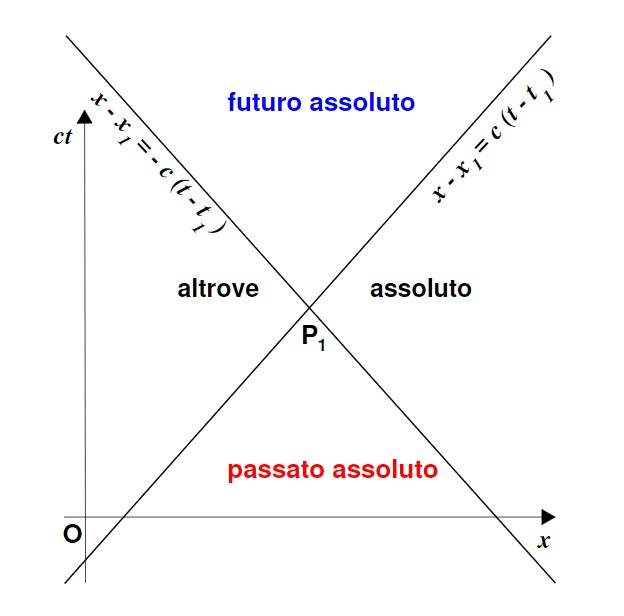
\includegraphics[scale=0.5]{./img/2020_03_20/minkowski.jpg}
	\caption{Spazio-Tempo di Minkowski unidimensionale relativo all'evento
		$\qvec{P}_1$ (origine)}
	\label{fig:minkowski}
\end{figure}

Le linee raffigurate rappresentano quelle che in una dimensione vengono
chiamate \textit{linee di luce} (in due dimensioni \textit{coni di luce}
ed in tre dimensioni \textit{iperconi di luce}). Le regioni dello spazio-tempo
interne alle linee di luce definiscono l'insieme degli eventi separati
dall'evento origine da distanze	di tipo tempo. Le regioni esterne alle linee di
luce, invece, definiscono l'insieme degli eventi separati dall'evento origine
da distanze di tipo spazio.

\section{Ulteriori Quadrivettori}
In aggiunta al quadrivettore posizione possiamo definire i seguenti
quadrivettori. Definiamo $t_0$ il \textbf{tempo proprio della particella},
ossia quello misurato nel sistema di riferimento che vede la particella in
quiete. Questo significa che\footnote{
	Tutte le variabili non apicate fanno riferimento al sistema di riferimento
	$K$ in moto relativo rispetto a $K^\prime$
}:
\begin{equation}
	\md{x}_0 = \md{y}_0 = \md{z}_0 = 0
	\mthen
	\md{s}^2 = c^2 \md{t}_0^2
\end{equation}
Dalla dilatazione temporale abbiamo:
\begin{equation}
	\md{t}_0 = \frac{\md{t}}{\gamma}
	\mthen
	\gamma = \mdv{t}{t_0}
\end{equation}
Quindi definiamo i seguenti quadrivettori:
\begin{itemize}
	\item \textbf{quadrivelocità}
	      \begin{equation}
		      \qvec{V} = \mdv{\qvec{X}}{t_0} = \mdv{\qvec{X}}{t} \mdv{t}{t_0} =
		      \gamma \mdv{\qvec{X}}{t}
		      \mthen
		      \boxed{
			      \qvec{V}
			      = \gamma\mdv{\qvec{X}}{t}
			      = \gamma \mcb{c,\vec{v}}
			      \equiv \mcb{\gamma c, \gamma \vec{v}}
		      }
	      \end{equation}
	      L'invariante della quadrivelocità:
	      \begin{equation}
		      \qvec{V}^2 = \gamma^2c^2 - \gamma^2\beta^2c^2 =
		      c^2\gamma^2\mrb{1-\beta^2} = c^2
	      \end{equation}

	\item \textbf{quadrimpulso}\footnote{
		      \textbf{Limite Classico}: per $\beta\to 0 \Rightarrow \gamma\to 1$ si
		      riottiene $\vec{p} = m\vec{v}$
	      }
	      \begin{equation}
		      \boxed{\qvec{P} = m \qvec{V} = m \gamma \mcb{c,\vec{v}}}
	      \end{equation}
	      con $m$ la \textit{massa a riposo} della particella.\par
	      L'invariante del quadrimpulso:
	      \begin{equation}
		      \qvec{P}^2 = m^2\gamma^2c^2 - m^2\gamma^2v^2 = m^2\gamma^2c^2 -
		      m^2\gamma^2\beta^2c^2 = m^2c^2\gamma^2\mrb{1-\beta^2} = m^2c^2
	      \end{equation}
\end{itemize}

\section{Energia}
\subsection{Energia a Riposo}
Definiamo l'energia a riposo di una particella come:
\begin{align}
	\textbf{Energia a riposo} \qquad \boxed{E_0 = m_0c^2}
\end{align}
dove $m_0$ è la massa a riposo della particella.

\subsection{Energia Relativistica}
Possiamo riscrivere il quadrimpulso come segue:
\begin{equation}
	\boxed{
		\qvec{P} = \mcb{\frac{E}{c}, \gamma\vec{p}}
	}
\end{equation}
dove $E$ è l'energia relativistica della particella e dove, per poter scrivere
la prima componente abbiamo sfruttato le seguenti identità:
\begin{equation}
	m_0 \gamma c = \frac{m_0 \gamma c^2}{c} = \frac{E_0\gamma}{c} = \frac{E}{c}
\end{equation}
\begin{align}
	\textbf{Energia Relativistica} \qquad \boxed{E = E_0\gamma = m_0 \gamma c^2}
\end{align}

\subsection{Energia Cinetica Relativistica}
Un altro modo per esprimere l'energia relativistica è come somma dell'energia a
riposo e dell'energia cinetica della particella, ovvero:
\begin{equation}
	E = E_0 + T
\end{equation}
Quindi segue che l'espressione esplicita dell'energia cinetica
relativistica\footnote{
	Attenzione: l'espressione dell'energia cinetica si può ricavare formalmente
	dal teorema delle forze vive utilizzando un'espressione relativisticamente
	corretta della forza (vedi Intro. Fisica Moderna)
}:
\begin{equation}
	\boxed{T = E - E_0 = m_0c^2\gamma - m_0c^2 = m_0c^2\mrb{\gamma - 1}}
\end{equation}

\subsubsection{Limite classico dell'energia cinetica}
Anche in questo caso, per riottenere l'espressione classica dell'energia
cinetica dobbiamo effettuare uno sviluppo al primo ordine del fattore $\gamma$
di Lorentz ($\gamma = 1 + \frac{1}{2}\beta^2$), quindi (ricordando la
definizione $\beta = \frac{v}{c}$):
\begin{equation}
	T_{\text{cl}} = mc^2\mrb{1+ \frac{1}{2}\beta^2 - 1} = \frac{1}{2}mc^2\beta^2 =
	\frac{1}{2}mv^2
\end{equation}

\section{Sistemi di due particelle}
Laddove possibile cercheremo di sfruttare gli invarianti relativistici
(\textit{invarianza della norma di un quadrivettore}), evitando il calcolo
delle trasformazioni di Lorentz per ottenere variabili cinematiche al passaggio
fra sistemi di riferimento.

Sfrutteremo in particolare:
\begin{itemize}
	\item utilizzo del \textit{principio di conservazione del quadrimpulso}:
	      \begin{equation}
		      \sum_{j=1}^{N_{\text{ini}}} P_j^{\text{ini}}
		      = \sum_{k=1}^{N_{\text{fin}}} P_k^{\text{fin}}
	      \end{equation}
	\item l'\textit{invariante relativistico associato} al quadrimpulso per
	      passare da un sistema di riferimento a un altro.
\end{itemize}
Negli esempi che seguono:
\begin{itemize}
	\item ricaveremo velocità e fattore di Lorentz,
	      $\gamma = \frac{1}{\sqrt{1 - \beta^2}}$, che ci portano dal \textit{sistema
		      di riferimento del laboratorio} al \textit{sistema di riferimento del
		      centro di massa} di due particelle;
	\item ricaveremo l'impulso e l'energia di una particella nel \textit{sistema
		      di riposo di un'altra};
	\item calcoleremo gli impulsi e le energie di due particelle \textit{nel
		      sistema del centro di massa} delle due particelle.
\end{itemize}

\begin{figure}[ht]
	\centering
	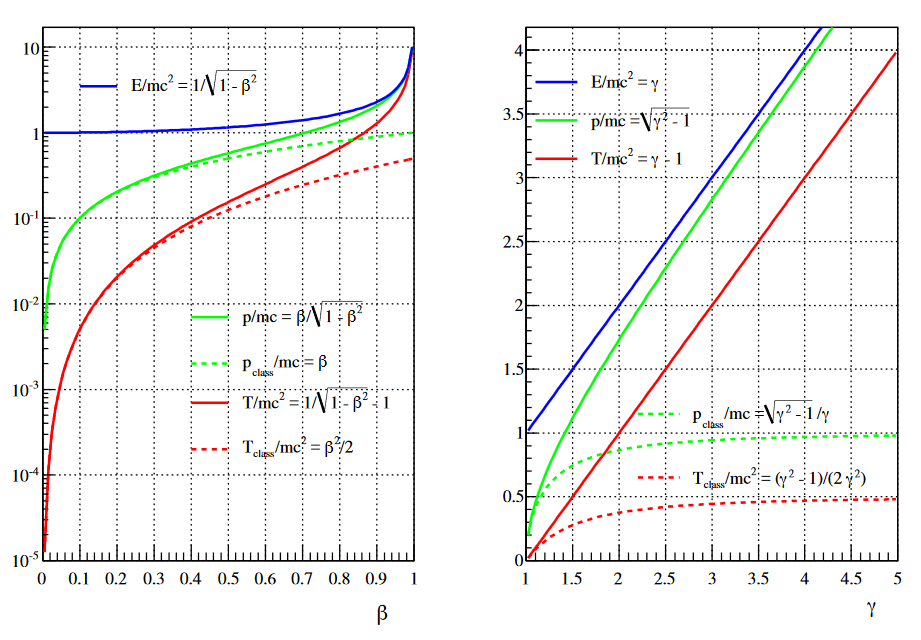
\includegraphics[scale=0.4]{./img/2020_03_20/realtivity_lectures.png}
	\caption{Energia totale, energia cinetica e impulso come funzioni di
		$\beta$ e $\gamma$ e rispettivi limiti classici ($\beta\to 0$)
	}
\end{figure}

\paragraph{Sistema di Unità Naturali}
D'ora in poi utilizzeremo il cosiddetto \textbf{sistema di unità naturali}, per
cui si fissano le costanti indicate di seguito pari all'unità:
\begin{equation}
	\boxed{\hbar = c = 1}
\end{equation}
e potremo scrivere \textit{uguaglianze fra grandezze fisiche non omogenee}
ricordandoci, però, di esprimere correttamente le unità di misura dei
risultati\footnote{
	Ad esempio, se un risultato di energia è $E = 1\si{\GeV}$, allora esprimeremo
	le grandezze $M,\vec{p}$ rispettivamente come $1\frac{\si{\GeV}}{c^2}$ e
	$1\frac{\si{\GeV}}{c}$
}.

Scriveremo il quadrimpulso come:
\begin{equation}
	\qvec{P} = \mcb{E,\vec{p}}
\end{equation}
e potremmo dire quindi:
\begin{equation}
	\qvec{P}^2 = E^2-\abs{\vec{p}\,}^2 = M^2
\end{equation}
\begin{equation}
	\textbf{Relazione di dispersione}
	\qquad
	\boxed{
		E^2 = \abs{\vec{p}\,}^2 + M^2
	}
\end{equation}
dove $M$ è detta \textbf{massa invariante} del sistema.

\subsection{Grandezze relative alla particella virtuale \quot{Centro di Massa}
	(CM)}
Le grandezze relative alle due particelle nel \textit{sistema del laboratorio}:
\begin{itemize}
	\item particella uno: $m_1,\ \qvec{P}_1$;
	\item particella due: $m_2,\ \qvec{P}_2$.
\end{itemize}
Nel sistema del laboratorio i due quadrimpulsi e i rispettivi invarianti
saranno:
\begin{equation}
	\qvec{P}_1 = \mcb{\varepsilon_1,\vec{p}_1}
	\mthen
	\qvec{P}_{1}^{2} = m_1^2
\end{equation}
\begin{equation}
	\qvec{P}_2 = \mcb{\varepsilon_2,\vec{p}_2}
	\mthen
	\qvec{P}_{2}^{2} = m_2^2
\end{equation}

\begin{note}[]
	D'ora in poi le quantità relative al sistema del centro di massa saranno
	espresse con un asterisco all'apice.
\end{note}

\begin{figure}[ht]
	\centering
	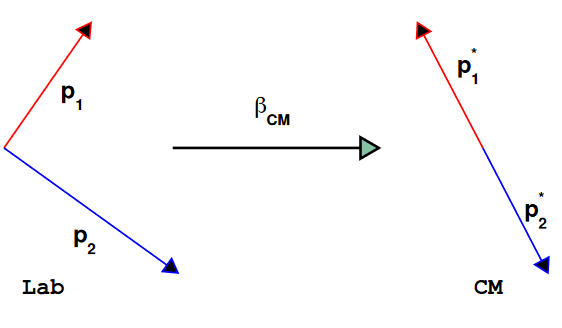
\includegraphics[scale=0.4]{./img/2020_03_20/particles1.png}
	\caption{Passaggio dal sistema del laboratorio al sistema del centro di massa
		\textbf{CM}}
	\label{fig:particles1}
\end{figure}

Il quadrivettore impulso totale, rispetto al \textit{sistema CM}:
\begin{equation}
	\qvec{P}^\ast
	= \qvec{P}_1^\ast + \qvec{P}_2^\ast
	= \mcb{\eps_1^\ast + \eps_2^\ast,\, 0}
\end{equation}
dato che nel sistema del centro di massa:
\begin{equation}
	\vec{p}_{1}^{\,\ast} + \vec{p}_{2}^{\,\ast} = 0
\end{equation}

Tramite una trasformazione di Lorentz del quadrimpulso si può riottenere
il quadrimpulso totale nel \textit{sistema del laboratorio}:
\begin{equation}
	\qvec{P}
	= \qvec{P}_1 + \qvec{P}_2
	= \mcb{\eps_1 + \eps_2,\, \vec{p}_1 + \vec{p}_2}
\end{equation}
Inoltre, per invarianza della norma, possiamo scrivere le seguenti
identità:
\begin{equation}
  \qvec{P}^2
	= E^{*2}
	= \mrb{\varepsilon_1^{\ast} + \varepsilon_2^{\ast}}^2
	= \mrb{\varepsilon_1 + \varepsilon_2}^2 - \mrb{\vec{p}_1 + \vec{p}_2}^2
\end{equation}
dove con $E ^{\ast}$ indichiamo l'\textbf{energia disponibile nel CM}.
Con $M$ la \textbf{massa invariante} totale del sistema, sfruttando
l'equazione precedente possiamo scrivere:
\begin{equation}
	\qvec{P}^2
	= \mrb{\qvec{P}_1 + \qvec{P}_2}^2
	= M^2
	= E^{\ast\,2}
	= \mrb{\varepsilon_1 + \varepsilon_2}^2 - \mrb{\vec{p}_1 + \vec{p}_2}^2
\end{equation}
Vediamo che massa invariante del sistema ed energia nel centro di massa
coincidono.

In questo modo abbiamo ridotto il problema di due particelle a un sistema di
\textbf{una sola particella virtuale \quot{centro di massa}} di quadrimpulso
$\qvec{P}$ ed massa $M = E^\ast$:
\begin{equation}
	\vec{p} = M\gamma\vec{\beta}_{\text{CM}}
\end{equation}
\begin{equation}
	E = M\gamma _{\text{CM}}
\end{equation}
dove $\vec{\beta}$ e $\gamma$ sono le velocità ed il fattore di Lorentz della
particella \textit{centro di massa} nel sistema del laboratorio:
\begin{equation}
	\boxed{\vec{\beta}_{\text{CM}}
	= \frac{\vec{p}}{E}
	= \frac{\vec{p}_1 + \vec{p}_2}{\varepsilon_1 + \varepsilon_2}}
	\label{eq:beta_CM}
\end{equation}
\begin{equation}
	\boxed{\gamma_{\text{CM}}
		= \frac{E}{M}
		= \frac{\varepsilon_1 + \varepsilon_2}{\sqrt{\mrb{\varepsilon_1 +
					\varepsilon_2}^2 - \mrb{\vec{p}_1 + \vec{p}_2}^2}}}
	\label{eq:gamma_CM}
\end{equation}

\subsection{Energia, impulso e velocità di una particella nel sistema di riposo
	dell'altra}
Nel sistema di riferimento $\textbf{RF}_1$, ovvero nel sistema di riferimento
solidale alla particella uno, i quadrivettori $\qvec{P}_1,\qvec{P}_2$:
\begin{equation}
	\qvec{P}_1 = \mcb{m_1,\, 0}
\end{equation}
\begin{equation}
	\qvec{P}_2 = \mcb{E_{2,1},\, \vec{p}_{2,1}}
\end{equation}

\begin{figure}[ht]
	\centering
	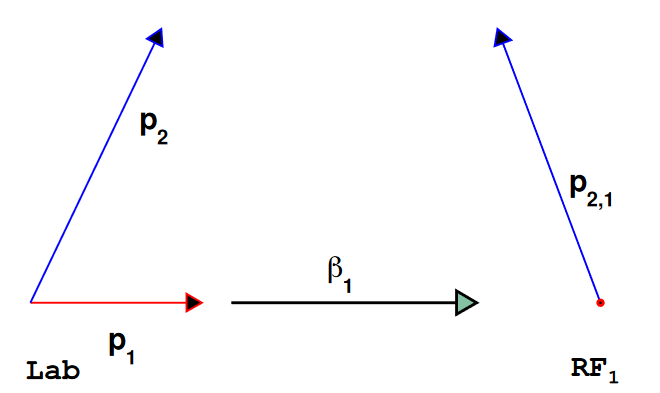
\includegraphics[scale=0.35]{./img/2020_03_20/relativity_lectures_1.png}
	\caption{Passaggio dal sistema del laboratorio al sistema di riferimento
		solidale alla particella uno, $\textbf{RF}_1$.}
\end{figure}

\begin{exercise}[]
	Dimostrare che il prodotto scalare fra quadrimpulsi è invariante
	relativistico.
\end{exercise}

\textit{Il prodotto scalare dei due quadrimpulsi è un invariante
	relativistico}, che vale:
\begin{equation}
	\qvec{P}_1 \qvec{P}_2 = m_1 E_{2,1}
	\mthen
	E_{2,1} = \frac{\qvec{P}_1 \qvec{P}_2}{m_1}
\end{equation}
inoltre, poiché possiamo scrivere:
\begin{equation}
	\abs{\vec{p}_{2,1}}^2 = E^2_{2,1} - m_2^2
\end{equation}
sostituendo l'espressione di $E _{2,1}$:
\begin{equation}
  \abs{\vec{p}_{2,1}}^2 = \frac{\qvec{P}_{1} \qvec{P}_{2}}{m_1} - m_2^2
\end{equation}
Per $\vec{\beta}_{2,1}$ possiamo scrivere:
\begin{equation}
  \abs{\vec{\beta}_{2,1}}^{2} = \frac{\abs{\vec{p}_{2,1}}^{2}}{E _{2,1}^{2}}
\end{equation}

Allora esprimiamo l'\textbf{energia}, l'\textbf{impulso} e la \textbf{velocità}
di una particella nel sistema di riposo dell'altra come, ovvero le grandezze
relative alla particella 2 nel sistema in cui la particella uno si trova in
quiete:
\begin{equation}
	\boxed{
		\begin{dcases}
			E_{2,1} = \frac{\qvec{P}_1\qvec{P}_2}{m_1}
			\\
			\abs{\vec{p}_{2,1}}^2
			= \frac{\mrb{\qvec{P}_{1} \qvec{P}_{2}}^{2}}{m_1^2} - m_2^2
			= \frac{\mrb{\qvec{P}_1\qvec{P}_2}^2 - m_1^2m_2^2}{m_1^2}
			\\
			\abs{\vec{\beta}_{2,1}}^2
			= \frac{\abs{\vec{p} _{2,1}}^{2}}{E _{2,1}^{2}}
			= \frac{\mrb{\qvec{P}_1\qvec{P}_2}^2 - m_1^2m_2^2}{\cancel{m_1^2}}
			\frac{\cancel{m_1^2}}{\mrb{\qvec{P}_{1} \qvec{P}_{2}}^{2}}
			= \frac{\mrb{\qvec{P}_1\qvec{P}_2}^2 -
				m_1^2m_2^2}{\mrb{\qvec{P}_1\qvec{P}_2}^2}
		\end{dcases}
	}
	\label{eq:sistema_riposo_altra}
\end{equation}
$\vec{\beta}_{2,1}$ rappresenta la \textit{velocità della particella due nel
	sistema di riferimento che vede la particella uno in quiete}.

 % Lezioni 2/3   A.A. 2022-2023
% %LTeX: language=it
\chapter{2020-03-24}
\section{Sistemi di due particelle (reprise)}
\subsection{Energia, Impulso e Velocità di una particella nel sistema CM}
È nostro scopo ora calcolare le grandezze energia, impulso e velocità delle due
particelle nel sistema di riferimento del centro di massa (CM).

Nel sistema del centro di massa consideriamo come particella a riposo la
particella fittizia \textit{centro di massa} ed utilizziamo le equazioni
\ref{eq:sistema_riposo_altra} considerando appunto come particella di
riferimento la particella \textit{centro di massa}.

Rispetto alle equazioni \ref{eq:sistema_riposo_altra} avremo quindi che
\footnote{
	$\vec{P}$ è riferito alla particella CM
}:
\begin{equation}
	\begin{dcases}
		\qvec{P}_1 \rightarrow \qvec{P} = \qvec{P}_1 + \qvec{P}_2
		\\
		\qvec{P}_2 \rightarrow \qvec{P}_i \qquad \mrb{i = 1,2}
	\end{dcases}
\end{equation}

Quindi riscriviamo il set di equazioni \ref{eq:sistema_riposo_altra}:
\begin{equation}
	\begin{dcases}
		\eps_i^\ast = \frac{\qvec{P} \qvec{P}_i}{M}
		\\
		\abs{\vec{p}_i^{\,\ast}}^2
		= \frac{\mrb{\qvec{P} \qvec{P}_i}^2- M^2m_i^2}{M^2}
		\\
		\abs{\vec{\beta}_i}^{\ast2}
		= \frac{\mrb{\qvec{P}\qvec{P}_i}^2- M^2m_i^2}{\mrb{\qvec{P} \qvec{P}_i}^2}
	\end{dcases}
\end{equation}

Ricordiamoci che $\qvec{P}_i = \mcb{m_i,\, \vec{p}_i}$. Ci interessa ora sapere
l'espressione esplicita di $\qvec{P} \qvec{P}_i$, quindi:
\begin{subequations}
	\begin{equation}
		\qvec{P} \qvec{P}_i
		= \mrb{\qvec{P}_1 + \qvec{P}_2} \qvec{P}_i
		= \qvec{P}_1 \qvec{P}_i + \qvec{P}_2 \qvec{P}_i
	\end{equation}
	e poiché $i = 1, 2$, dunque:
	\begin{equation}
		\qvec{P} \qvec{P}_i
		= \qvec{P}_1 \qvec{P}_2 + \qvec{P}_i^2
		= \qvec{P}_1 \qvec{P}_2 + m_i^2
		= \frac{1}{2} \msb{M^2 - m_1^2 - m_2^2} + m_i^2
	\end{equation}
	Il primo termine della somma:
	\begin{equation}
		\qvec{P}_1 \qvec{P}_2
		= \frac{1}{2} \msb{\mrb{\qvec{P}_1 + \qvec{P}_2}^2 - \qvec{P_1}^2 -
			\qvec{P_2}^2}
		= \frac{1}{2} \msb{M^2 - m_1^2 - m_2^2}
	\end{equation}
	dove abbiamo sfruttato le relazioni fra la norma del quadrimpulso e la massa
	delle particelle. Sostituendo nell'equazione precedente si ottiene:
	\begin{equation}
		\boxed{
			\qvec{P} \qvec{P}_i
			= \frac{1}{2} \mrb{M^2 + m_i^2 - m_j^2} \qquad i,j
			= 1,2 \quad \text{e},
			\quad i\neq j
		}
	\end{equation}
\end{subequations}

Per le \textbf{energie} viste dal sistema del centro di massa:
\begin{equation}
	\boxed{\begin{dcases}
			\eps_1^\ast = \frac{M^2 + m_1^2 - m_2^2}{2M} \\
			\eps_2^\ast = \frac{M^2 + m_2^2 - m_1^2}{2M}
		\end{dcases}}
\end{equation}
vediamo che, nonostante nel sistema del centro di massa le due particelle
abbiano lo stesso impulso (in modulo), le energie sono diverse, causa le diverse
masse.

Osserviamo che la loro somma dovrebbe fornire la massa invariante $M$, infatti:
\begin{equation}
	\eps_1^\ast + \eps_2^*
	= \frac{M^2 + m_1^2 - m_2^2 + M^2 + m_2^2 - m_1^2}{2M}
	= \frac{2M^2}{2M}
	= M
\end{equation}

Per gli \textbf{impulsi} (\textit{trivettori}) visti dal sistema del centro di
massa:
\begin{equation}
	\abs{\vec{p}_{1}^{\ast}}^{2} = \frac{\mrb{M^2 + m_1^2 - m_2^2}^{2} - 4 M^2
		m_1^2}{4M^2}
\end{equation}
e analogamente per $\abs{\vec{p}_{2}^{\ast}}^{2}$, quindi svolgendo i calcoli:
\begin{equation}
	\boxed{
	\abs{\vec{p}^{\,\ast}}^2
	= \abs{\vec{p}_1^{\,\ast}}^2
	= \abs{\vec{p}_2^{\,\ast}}^2
	= \frac{\msb{M^2 - \mrb{m_1 + m_2}^2}\msb{M^2 - \mrb{m_1 - m_2}^2}}{4M^2}
	}
\end{equation}

\begin{example}[]
	Dimostrare che effettuando una trasformazione di Lorentz al CM si ottiene:
	\begin{equation}
		\vec{p}_1^{\,\ast} + \vec{p}_2^{\,\ast} = 0
	\end{equation}

	\begin{note}[]
		Ricordiamo che le quantità relative al SR del centro di massa sono indicate
		con il simbolo $\ast$.
	\end{note}

	Dimostriamo questa relazione utilizzando le trasformazioni di Lorentz nella
	forma vettoriale (equazione \ref{eq:lorentz_vettoriale}) e trasformiamo
	l'impulso come segue:
	\begin{equation}
		\vec{p}^{\,\ast} = \vec{p} - \vec{\beta}\gamma \msb{\frac{\gamma}{\gamma +
				1} \mrb{ -\vec{\beta} \cdot \vec{p}} + \eps} = \vec{p} + \vec{\beta}\gamma
		\msb{\frac{\gamma}{\gamma + 1} \mrb{\vec{\beta} \cdot \vec{p}} - \eps}
	\end{equation}

	Quindi scriviamo la trasformazione dell'impulso somma:
	\begin{equation}
		\vec{p}_1^{\,\ast} + \vec{p}_2^{\,\ast} = \vec{p}_1 + \vec{p}_2 +
		\vec{\beta}\gamma \msb{\frac{\gamma}{\gamma+1} \vec{\beta} \cdot
			\mrb{\vec{p}_1 + \vec{p}_2} - \mrb{\eps_1 + \eps_2}}
	\end{equation}
	Sfruttando il risultato dell'equazione \ref{eq:beta_CM}, sostituendo:
	\begin{equation}
		\vec{p}_1^{\,\ast} + \vec{p}_2^{\,\ast} = \vec{\beta} \mrb{\eps_1 +
			\eps_2} + \abs{\vec{\beta}}^2 \frac{\gamma^2}{\gamma + 1}
		\vec{\beta}\mrb{\eps_1 + \eps_2} - \gamma\vec{\beta}
	\end{equation}
	mettiamo in evidenza $\vec{\beta}\mrb{\eps_1 + \eps_2}$:
	\begin{equation}
		\vec{p}_1^{\,\ast} + \vec{p}_2^{\,\ast} = \vec{\beta}\mrb{\eps_1 +
			\eps_2} \msb{1 + \abs{\vec{\beta}}^2 \frac{\gamma^2}{\gamma + 1} -
			\gamma}
	\end{equation}
	Sfruttando la relazione:
	\begin{equation}
		\abs{\vec{\beta}}^2 = \frac{\gamma^2 - 1}{\gamma^2} = \frac{\mrb{\gamma -
				1} \mrb{\gamma + 1}}{\gamma^2}
	\end{equation}
	possiamo concludere quanto segue:
	\begin{align}
		\vec{p}_1^{\,\ast} + \vec{p}_2^{\,\ast}
		 & = \vec{\beta}\mrb{\eps_1 + \eps_2} \msb{1 + \frac{\mrb{\gamma - 1}
				\cancel{\mrb{\gamma + 1}}}{\cancel{\gamma^2}}
			\frac{\cancel{\gamma^2}}{\cancel{\gamma + 1}} - \gamma}
		\\\notag
		 & = \vec{\beta}\mrb{\eps_1 + \eps_2} \msb{\cancel{1} + \cancel{\gamma} -
			\cancel{1} - \cancel{\gamma}}
		\\\notag
		 & = 0
	\end{align}
	Quindi abbiamo dimostrato quanto era richiesto.
\end{example}

\begin{exercise}
	All'interno del nucleo, i nucleoni si muovono con energie cinetica
	dell'ordine di $\qty{20}{\MeV}$.
	Studiare gli effetti cinematici di questo movimento quando protoni di energia
	cinetica di $\qty{200}{\GeV}$ urtano i nucleoni nei casi in cui questi si
	muovano in direzione \textit{parallela} e \textit{antiparallela} ai protoni
	del fascio.
	Consideriamo per semplicità la massa dei nucleoni $\SI{1}{\frac{\GeV}{c^2}}$.
	\begin{enumerate}
		\item Calcolare la differenza di energia nel centro di massa nei casi
		      \textit{parallelo} e \textit{antiparallelo}.
		\item Quale energia dovrebbero avere i protoni incidenti per trovare la
		      stessa energia nel centro di massa se urtassero nucleoni a riposo?
	\end{enumerate}

	Il quadrimpulso totale nel caso \textit{parallelo}:
	\begin{equation}
		\qvec{P} = \Set{E_p + E_n, p_p + p_n, 0, 0}
	\end{equation}
	e nel caso \textit{antiparallelo}:
	\begin{equation}
		\qvec{P} = \Set{E_p + E_n, p_p - p_n, 0, 0}
	\end{equation}
	L'\textit{energia disponibile nel centro di massa} (invariante):
	\begin{align}
		\qvec{P}^2
		 & = E ^{\ast\, 2}
		\\\notag
		 & = \mrb{E_n + E_p}^{2} - \mrb{p_p \pm p_n}^{2}
		\\\notag
		 & = E_n^2 + E_p^2 + 2 E_p E_n - p_p^2 - p_n^2 \mp 2 p_p p_n
		\\\notag
		 & = \cancel{p_n^2} + m_n^2 + \cancel{p_p^2} + m_p^2 + 2 E_p E_n
		- \cancel{p_p^2} - \cancel{p_n^2} \mp 2 p_p p_n
		\\\notag
		 & = 2 m_n^2 + 2 E_p E_n \mp 2 \sqrt{\mrb{E_p^2 - m_n^2}\mrb{E_n^2 - m_n^2}}
	\end{align}
	dove nell'ultimo passaggio abbiamo considerato le masse dei nucleoni uguali
	in approssimazione $m_p = m_n$ e abbiamo sfruttato l'equazione
	$p_p p_n = \sqrt{\mrb{E_p^2 - m_n^2}\mrb{E_n^2 - m_n^2}}$.
	Indicando con $T_x$ l'energia cinetica:
	\begin{equation}
    T_p:
		\qquad
		E_p
		= T_p + m_n
		= \qty{200}{\GeV} + \qty{1}{\GeV}
		= \qty{201}{\GeV}
	\end{equation}
	\begin{equation}
    T_n:
		\qquad
		E_n
		= T_n + m_n
		= \qty{20}{\MeV} + \qty{1}{\GeV}
		= \qty{1.02}{\GeV}
	\end{equation}
	Quindi:
	\begin{equation}
		E ^{\ast\, 2} = 2 \mrb{1^2 + \numproduct[
				product-symbol = \ensuremath{\cdot}
			]{201 x 1.02} \mp 40.4} \unit{\GeV^2}
		= \begin{dcases}
			\qty{331.24}{\GeV^2}, \quad \textit{Parallelo}
			\\
			\qty{492.92}{\GeV^2}, \quad \textit{Antiparallelo}
		\end{dcases}
	\end{equation}
	allora:
	\begin{equation}
		E ^{\ast}
		= \begin{dcases}
			\qty{18.2}{\GeV}, \quad \textit{Parallelo}
			\\
			\qty{22.2}{\GeV}, \quad \textit{Antiparallelo}
		\end{dcases}
	\end{equation}

	Rispondendo alla seconda domanda:
	\begin{equation}
		\qvec{P}_n = \Set{E_n, 0, 0, 0}
	\end{equation}
	quindi:
	\begin{equation}
		E_n = \sqrt{\cancel{p_n^2} + m_n ^{2}} = m_n
	\end{equation}
	Dunque:
	\begin{equation}
		E_p \rightarrow E_p \mprime:
		\qquad
		E ^{\ast\, 2}
		= 2 m_n^2 + 2 E_p \mprime E_n \mp 2 \sqrt{\mrb{E_p^2 - m_n^2} \cancel{\mrb{m_n^2 - m_n^2}}}
		= 2 m_n^2 + 2 E_p \mprime E_n
	\end{equation}
	Allora scriviamo:
	\begin{equation}
		2 E_p \mprime E_n = E ^{\ast\, 2} - m_n^2
		\mthen
		E_p \mprime
		= \frac{1}{2 m_n} \msb{E ^{\ast`, 2} - 2 m_n^2}
		= \frac{E ^{\ast\, 2} - 2}{2}
	\end{equation}
	Infine:
	\begin{equation}
		E _{p} \mprime
		= \begin{dcases}
			???, \quad \textit{Parallelo}
			\\
			\qty{245}{\GeV}, \quad \textit{Antiparallelo}
		\end{dcases}
	\end{equation}
\end{exercise}

\section{Decadimento in due corpi}
Trattiamo ora il caso di una particella $\boldsymbol{A}$ che decade in due
particelle $\boldsymbol{B}$ e $\boldsymbol{C}$ (figura
\ref{fig:decadimento_due_corpi}) nel sistema del centro di massa (CM).
L'energia disponibile nel centro di massa è proprio l'energia a riposo della
particella iniziale $\boldsymbol{A}$ ed è la quantità  $E^\ast = M$.
Dopo il decadimento, chiaramente: $M \rightarrow m_1 + m_2$.

\begin{figure}[ht!]
	\centering
	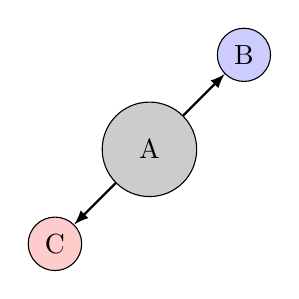
\begin{tikzpicture}[scale=0.8]
		\node[circle, draw, fill=black!20, minimum size = 1.2cm] (A) at (0,0) {A};
		\node[circle, draw, fill=blue!20, minimum size = 0.4cm] (B) at (1.5,1.5) {B};
		\node[circle, draw, fill=red!20, minimum size = 0.4cm] (C) at (-1.5,-1.5) {C};

		\draw[-latex, thick] (A)--(B);
		\draw[-latex, thick] (A)--(C);
	\end{tikzpicture}
	\caption{Schema del decadimento in due corpi nel sistema del centro di massa}
	\label{fig:decadimento_due_corpi}
\end{figure}

Per il sistema vale:
\begin{equation}
	\begin{dcases}
		\vec{p}_1 + \vec{p}_2 = 0
		\\
		\eps_1^\ast + \eps_2^\ast = E ^{\ast} = M
	\end{dcases}
\end{equation}
dove:
\begin{equation}
	\eps_1^\ast = \frac{M^2 + \mrb{m_1 + m_2}^2}{2M};
	\qquad
	\eps_2^\ast = \frac{M^2 + \mrb{m_1^2 - m_2^2}}{2M}
\end{equation}
\begin{equation}
	\abs{\vec{p}^{\,\ast}}^2
	= \abs{\vec{p}_{1}^{\ast}}^{2}
	= \abs{\vec{p}_{2}^{\ast}}^{2}
	= \frac{\msb{M^2 - \mrb{m_1 + m_2}^2} \msb{M^2 -
			\mrb{m_1 - m_2}^2}}{4M^2}
	\label{eq:modulo_quadro_impulso}
\end{equation}

\begin{note}[]
	In questo schema di decadimento abbiamo considerato una distribuzione
	\textit{isotropa} degli impulsi risultati dal decadimento. Questa condizione
	d'isotropia, tuttavia, può essere fortemente alterata dalla dinamica interna
	del sistema, che noi in questo caso stiamo trascurando. Questo vuol dire che
	non è detto che la direzione degli impulsi risultanti sia soggetta a una
	condizione d'isotropia.
\end{note}

\begin{example}[]
	Consideriamo il caso di un decadimento di un \textit{pione positivo} $\pi^+$
	in un \textit{muone positivo} $\mu^+$ e in un \textit{neutrino muonico}
	$\nu_\mu$:
	\begin{equation}
		\pi^+ \longrightarrow \mu^+ + \nu_\mu
	\end{equation}
	Le masse delle particelle:
	\begin{align}
		m_\pi = \qty{140}{\MeV\per c^2};
		\qquad
		m_\mu = \qty{106}{\MeV\per c^2};
		\qquad
		m_\nu = \qty{0}{\MeV\per c^2}
	\end{align}
	Sfruttando i risultati che abbiamo ricavato fino a ora, nel sistema del
	centro di massa abbiamo:
	\begin{subequations}
		\begin{equation}
			\abs{\vec{p}_\mu^{\,\ast}}^2 = \abs{\vec{p}_\nu^{\,\ast}}^2
			= \frac{
				\msb{m_\pi^2 - \mrb{m_\mu^2 + \cancel{m _{\nu}^{2}}}}
				\mrb{m_\pi^2 - \mrb{m_\mu^2 - \cancel{m _{\nu}^{2}}}}
			}{4m_\pi^2}
			= \frac{\mrb{m_\pi^2 - m_\mu^2}\mrb{m_\pi^2 - m_\mu^2}}{4m_\pi^2}
			= \frac{\mrb{m _{\pi}^{2} - m _{\mu}^{2}}^{2}}{4 m _{\pi}^{2}}
		\end{equation}
		\begin{equation}
			\Rightarrow \abs{\vec{p}_\mu^{\,\ast}}
			= \abs{\vec{p}_\nu^{\,\ast}}
			= \frac{m_\pi^2 - m_\mu^2}{2m_\mu}
			= \frac{140^2-106^2}{\numproduct[
					product-symbol = \ensuremath{\cdot}
				]{2 x 140}}\si{\MeV\per c}
			\simeq \qty{30}{\MeV\per c}
		\end{equation}
	\end{subequations}

	Per le energie abbiamo:
	\begin{equation}
		\eps_\mu = \sqrt{\abs{\vec{p}_\mu^{\,\ast}}^2 + m_\mu^2}
		\simeq \qty{110}{\MeV};
		\qquad
		\eps_\nu = \sqrt{\abs{\vec{p}_\nu^{\,\ast}}^2 + m_\nu^2}
		\simeq \qty{30}{\MeV}
	\end{equation}
\end{example}

\begin{example}[]
  Consideriamo il caso del decadimento della particella $\Lambda$\footnote{
    $\Lambda$ è una particella neutra; In tutte le reazioni valgono:
    \begin{itemize}
      \item \textit{principio di conservazione della carica}
      \item \textit{principio di conservazione del numero leptonico}
      \item \textit{principio di conservazione del numero barionico}
    \end{itemize}
  }:
	\begin{equation}
		\Lambda \rightarrow p + \pi ^{-}
	\end{equation}
  Date le masse:
  \begin{equation}
    m _{\Lambda} = \qty{1116}{\MeV \per c^2};
    \qquad
    m_p = \qty{938}{\MeV \per c^2};
    \qquad
    m _{\pi^-} = \qty{140}{\MeV \per c^2}
  \end{equation}
	Abbiamo, nel sistema di riposo della particella $\Lambda$ che decade, che
  coincide con il sistema del centro di massa:
	\begin{equation}
		\abs{\vec{p}_{p}^{\,\ast}}^{2}
		= \abs{\vec{p}_{\pi^-}^{\,\ast}}^{2}
		= \frac{
			\msb{m _{\Lambda} ^{2} - \mrb{m _{p} + m _{\pi}}^{2}}
			\msb{m _{\Lambda} ^{2} - \mrb{m _{p} - m _{\pi}}^{2}}
		}{4 M _{\Lambda}^{2}}
    \simeq \qty{101}{\MeV \per c}
	\end{equation}
\end{example}
 % Lezioni 3/4   A.A. 2022-2023
% %LTeX: language=it
\chapter{Lezione 26/03/2020}
\section{Soglia di una reazione}
Discutiamo ora le reazioni che possono avvenire solo superando la cosiddetta
\textbf{soglia di reazione}.

Dall'equazione \ref{eq:modulo_quadro_impulso}, poiché
$\abs{\vec{p}^{\,\ast}}^2$ è una quantità positiva, allora dovrà
necessariamente valere:
\begin{equation}
	M \geq m_1 + m_2
\end{equation}
\textit{Affinché un decadimento possa avvenire, le masse (invarianti) delle due
	particelle prodotto devono essere al più (sommate) pari alla massa della
	particella che decade (se emesse a riposo) o minori, e in tal caso l'energia
	associata alla \quot{massa in eccesso} si traduce in impulso delle due
	particelle prodotto}.

La relazione appena indicata definisce la \textbf{soglia di reazione} e in
modo generale si può scrivere:
\begin{align}
	\textbf{Soglia di Reazione}
	\quad
	\boxed{
	\qvec{P}^2 = \mrb{\qvec{P}_1 + \qvec{P}_2}^2 \geq
	\mrb{\sum_{f=1}^{N_\text{fin}} m_f}^2
	}
	\label{eq:soglia_reazione}
\end{align}

\begin{example}[Soglia della fotoproduzione del pione neutro]
	La reazione di \textit{fotoproduzione del pione neutro}, con targhetta di
	protoni a riposo $\vec{p}_{p} = 0$, è la seguente:
	\begin{equation}
		\gamma + p \longrightarrow p + \pi^0
	\end{equation}
	dove con $\gamma$ si indica il fotone incidente sul protone bersaglio $p$ e
	$\pi^0$ il pione neutro. Le masse:
	\begin{equation}
		m_p = \qty{938}{\MeV \per c^2};
		\\
		m_{\pi^0} = \qty{135}{\MeV \per c^2};
	\end{equation}

	\begin{note}[]
		La massa del pione neutro è inferiore rispetto a quella del pione carico
	\end{note}

	I relativi quadrimpulsi iniziali:
	\begin{equation}
		\qvec{P}_\gamma = \Set{E_\gamma, E_\gamma};
		\qquad
		\qvec{P}_p = \Set{m_p, 0}
	\end{equation}
	L'impulso iniziale del protone è nullo supponendo il protone bersaglio
	inizialmente fermo (questa è ovviamente un'approssimazione).
	L'equazione \ref{eq:soglia_reazione} che descrive la soglia della reazione
	diventa in questo caso:
	\begin{align}
		\mrb{\qvec{P}_\gamma + \qvec{P}_p}^2
		 & = \mrb{E_\gamma + m_p}^2 - E_\gamma^2
		\\\notag
		 & = \cancel{E_\gamma^2} + m_p^2 + 2 E_\gamma m_p - \cancel{E_\gamma^2}
		\\\notag
		 & = m_p\mrb{2E_\gamma + m_p}
		\\\notag
		 & \geq \mrb{m_p + m_{\pi^0}}^2
	\end{align}
	dove abbiamo utilizzato il fatto che il fotone abbia massa nulla\footnote{
		Infatti esprimendo esplicitamente l'impulso del fotone $\vec{p}_\gamma =
			\sqrt{E_\gamma^2 - \cancel m_\gamma^2} = E_\gamma$
		il quadrimpulso si riduce a
		$\qvec{P} = \Set{E _{\gamma}, \vec{p}_{\gamma}} = \Set{E _{\gamma}, E
					_{\gamma}}$
	}.
	Quindi definendo $E_\gamma^{\mrb{s}}$ l'\textit{energia di soglia} della
	reazione, possiamo dire che la reazione avviene se l'energia del fotone
	$\gamma$ è tale che:
	\begin{equation}
		E_\gamma
		\geq E_\gamma^{\mrb{s}}
		= \frac{\mrb{m_p + m_{\pi^0}}^2 - m_p^2}{2m_p}
		\simeq \qty{145}{\MeV}
	\end{equation}
\end{example}

\begin{example}[Soglia al collider]
	A differenza degli esperimenti a targhetta fissa, se i fasci di particelle
	hanno la stessa massa e impulsi uguali e contrari. Al collider il sistema del
	centro di massa coincide con il sistema del laboratorio.

	Consideriamo la collisione di un fascio di elettroni ed un fascio di
	positroni:
	\begin{equation}
		e^+ + e^- \rightarrow \mu^+ + \mu^-
	\end{equation}
	I quadrimpulsi:
	\begin{equation}
		\qvec{P _{e^-}} = \Set{E _{e^-}, \vec{p}_{e^-}};
		\qquad
		\qvec{P _{e^+}} = \Set{E _{e^+}, \vec{p}_{e^+}}
	\end{equation}
	Quindi, considerando che $\vec{p}_{e^+} = - \vec{p}_{e^-}$:
	\begin{align}
		\mrb{\qvec{P}_{e^+} + \qvec{P}_{e^-}}^{2}
		 & = \mrb{E _{e^+} + E _{e^-}}^{2} - \cancel{\mrb{\vec{p}_{e^+} +
				\vec{p}_{e^-}}}
		\\\notag
		 & = E _{e^+}^{2} + E _{e^-}^{2} + 2 E _{e^+} E _{e^-}
		\\\notag
		 & = \mrb{2 E _{e}}^{2} \geq \mrb{2 m _{\mu}}^{2}
	\end{align}
	Quindi l'energia di soglia:
	\begin{equation}
		E _{e}^{\mrb{S}} = m _{\mu} = \qty{106}{\MeV}
	\end{equation}
\end{example}

\subsection{Esperimenti a bersaglio fisso}
Nel caso di esperimenti a bersaglio fisso, dove consideriamo l'impulso della
particella bersaglio nullo (\textit{bersaglio fermo}), l'espressione di soglia
assume una forma utile se espressa in termini di \textbf{energia
	cinetica}\footnote{
	In unità naturali l'espressione relativistica dell'energia
	cinetica è $T = E - m$
}.
Definendo $p$ la particella \textit{proiettile} e $B$ la particella
\textit{bersaglio}, consideriamo la reazione:
\begin{equation}
	p + B \longrightarrow 1 + 2 + \cdots + N_\text{fin}
\end{equation}
allora abbiamo\footnote{
	Stiamo considerando la particella bersaglio ferma, quindi
	$E_B = m_p$
}:
\begin{itemize}
	\item \textbf{stato iniziale}, \textit{prima dell'urto} (poiché il bersaglio
	      è supposto fermo la sua energia sarà l'energia a riposo, quindi
	      $E_B \equiv m_B$ è l'impulso nullo
	      $p_B = 0$):
	      \begin{align}
		      \label{eq:soglia_cinetica_iniziale}
		      \qvec{P}^2
		       & = \mrb{E_p^2 + E_B^2} - \abs{\vec{p}_p + \vec{p}_{B}}^2
		      \\\notag
		       & = \mrb{E_p^2 + m_B^2} - \abs{\vec{p}_p}^2
		      \\\notag
		       & = \cancel{E_p^2} + m_B^2 + 2 E_p m_B - \cancel{E_p^2} + m_p^2
		      \\\notag
		       & = m_p^2 + m_B^2 + 2 m_B E_B
		      \\\notag
		       & = m_p^2 + m_B^2 + 2 m_B \mrb{T_p + m_p}
		      \\\notag
		       & = m_p^2 + m_B^2 + 2 m_B m_p + 2 m_B T_p
		      \\\notag
		       & = \mrb{m_p + m_B}^2 + 2 m_B T_p
	      \end{align}
	\item \textbf{stato finale}, \textit{dopo l'urto}:
	      \begin{equation}
		      \qvec{P}^2
		      = \mrb{\sum_{f=1}^{N_\text{fin}} E_f^*}^2
		      = \mrb{\sum_{f=1}^{N_\text{fin}} \msb{T_f^* + m_f}}^2
		      \geq \mrb{\sum_{f=1}^{N_\text{fin}} m_f}^2
		      \label{eq:soglia_cinetica_finale}
	      \end{equation}
	      Poiché la \textbf{condizione di soglia} è data dall'uguaglianza, allora
	      abbiamo che per tale condizione tutte le energie cinetiche sono
	      nulle\footnote{
		      Particelle create ferme nel centro di massa CM del sistema
	      }.
\end{itemize}

Poiché $\qvec{P}^2$ è un \textit{invariante relativistico}, uguagliando gli
ultimi termini delle equazioni \ref{eq:soglia_cinetica_iniziale} e
\ref{eq:soglia_cinetica_finale} e imponendo che $T_p$ sia proprio l'energia
cinetica di soglia:
\begin{equation}
	\mrb{m_p + m_B}^2 + 2 m_B T_p = \mrb{\sum_{f=1}^{N_\text{fin}} m_f}^2
\end{equation}
con $T_p \equiv T_p^{\mrb{s}}$.
Fatte queste considerazioni possiamo quindi scrivere che per la condizione di
soglia varrà:
\begin{equation}
	\textbf{Energia Cinetica di Soglia}
	\qquad
	\boxed{T_p^{\mrb{s}} = \frac{\mrb{\sum_f m_f}^2 - \mrb{m_p + m_B}^2}{2 m_B}}
\end{equation}

\begin{note}[]
	Per ottenere l'energia cinetica di soglia abbiamo sfruttato
	l'\textit{invariante} relativistico $\qvec{P}^{2}$ e la \textit{conservazione
		del quadrimpulso}.
\end{note}

\begin{example}[Produzione di coppie]
	Soglia per la produzione di coppie (indicando con $N$ i nuclei):
	\begin{equation}
		\gamma + N \rightarrow N + e^+ + e^-
	\end{equation}
	è una reazione che \textit{non può avvenire in vuoto}\footnote{
		La reazione
		\[
			\gamma \rightarrow e^+ + e^-
		\]
		non può avvenire. Infatti dato che
		$\qvec{P}_{\gamma} = \Set{E _{\gamma}, E _{\gamma}}$:
		\[
			\qvec{P}^2_\text{ini} = 0 \neq \qvec{P}^2_\text{fin} = \mrb{E
					_{e^-}^{\ast} + E _{e^+}^{\ast}}^{2} \geq \mrb{2 m_e}^{2}
		\]
	}
	La soglia della reazione è la seguente:
	\begin{equation}
		T _{\gamma} ^{\mrb{s}} = E _{\gamma} ^{\mrb{s}} = \frac{\mrb{M + 2 m
					_{e^-}}^{2} - M^2}{2M}
	\end{equation}
	Un'altra cosa che possiamo notare è la seguente. La massa dell'elettrone è
	$m _{e^-} = \SI{0.511}{\MeV \per c^2}$; indicando con $A$ il numero di
	nucleoni e $m_n$ la massa del nucleone, la massa del nucleo sarà $M = A m_n =
		A \cdot \SI{1000}{\MeV \per c^2}$. Quindi abbiamo che $M \gg m _{e^-}$,
	ma non \textit{possiamo dire che la soglia della reazione è nulla}!
	Dobbiamo sviluppare:
	\begin{equation}
		E _{\gamma} ^{\mrb{s}} = \frac{\cancel{M^2} + 4 m _{e^-}^{2} + 4 M m _{e^-}
			- \cancel{M^2}}{2M} \simeq \frac{\cancel{4M}m _{e^-}}{\cancel{2M}} = 2 m
			_{e^-} \simeq \SI{1}{\MeV}
	\end{equation}
\end{example}

\begin{example}[Produzione di antiprotoni]
  Vediamo ora la \textit{soglia per la produzione di antiprotoni}\footnote{
    Deve valere la \textit{conservazione del numero barionico}
  }.
	\begin{equation}
		p + p \rightarrow p + p + p + \cc{p}
	\end{equation}
	Ammesso che questa reazione sia permessa dalla dinamica della produzione di
	antiprotoni, vogliamo calcolare quale sia la soglia minima per la produzione
	di antiprotoni\footnote{
		Le masse delle antiparticelle sono le medesime di quelle delle
		corrispondenti particelle
	} (la massa del protone/antiprotone è $m _{p} = m _{\cc{p}} \simeq
	\SI{0.940}{\GeV \per c^2}$):
	\begin{equation}
		T _{p} ^{\mrb{s}} = \frac{\mrb{4 m_p}^{2} - \mrb{2 m_p}^{2}}{2 m_p} = 6 m_p
		\simeq \qty{5.9}{\GeV}
	\end{equation}
\end{example}

\section{Angolo di apertura di un decadimento in due corpi}
Supponiamo di essere in presenza di un fenomeno di decadimento in due corpi
visto dal sistema di riferimento del laboratorio (\textbf{Lab}) di una
particella iniziale di massa $M$ in due particelle $a,b$:
\begin{equation}
	M \rightarrow a + b
\end{equation}
Sia $\theta$ l'angolo
di apertura fra gli impulsi $\vec{p}_a$ e $\vec{p}_b$ delle particelle prodotte
dalla reazione e $\qvec{P}_a = \Set{E_a, \vec{p}_{a}}$ e $\qvec{P}_b =
	\Set{E_b, \vec{p}_{b}}$ i quadrimpulsi delle due particelle risultanti dalla
reazione:
\begin{subequations}
	\begin{align}
		\qvec{P}^2
    &= M^2
    \\\notag
    &= \mrb{\qvec{P}_a + \qvec{P}_b}^2
    \\\notag
    &= \mrb{E_a + E_b}^{2} - \abs{\vec{p}_{a} + \vec{p}_{b}}^{2}
    \\\notag
    &= E_a^{2} + E_b^{2} + 2 E_a E_b - \abs{\vec{p}_{a}}^{2} -
    \abs{\vec{p}_{b}}^{2} - 2 \abs{\vec{p}_{a}} \abs{\vec{p _{b}}} \cos \theta
    \\\notag
    &= m_a^2 + m_b^2 + 2 E_a E_b - 2 \abs{\vec{p}_a}\abs{\vec{p}_b} \cos \theta
	\end{align}
	\begin{equation}
		\Rightarrow \cos \theta = \frac{m_a^2 + m_b^2 - M^2 + 2 E_a E_b}{2
			\abs{\vec{p}_a}\abs{\vec{p}_b}}
	\end{equation}
\end{subequations}
Nell'ipotesi che le particelle $a,b$ prodotte siano particelle
\textbf{ultrarelativistiche}, ovvero particelle per cui $E_a \gg m_a$ e $E_b
	\gg m_b$, la precente espressione si semplifica in\footnote{
	Poiché in tale approssimazione $\abs{\vec{p}_\alpha} = \sqrt{E_\alpha^2 -
			m_\alpha^2} \sim E_\alpha$ con $\alpha = a, b$
}:
\begin{subequations}
	\begin{equation}
		\cos \theta = \frac{m_a^2 + m_b^2 - M^2}{2 E_a E_b} + 1
	\end{equation}
	\begin{equation}
		\Rightarrow 1 - \cos \theta = \frac{M^2 - m_a^2 - m_b^2}{2 E_a E_b}
	\end{equation}
\end{subequations}
che, essendo $1 - \cos \theta = 2 \sin^2 \frac{\theta}{2}$, diventa:
\begin{equation}
	\sin \frac{\theta}{2} = \sqrt{\frac{M^2 - m_a^2 - m_b^2}{4 E_a E_b}}
\end{equation}

Ora se $E$ è l'energia della particella che decade nel sistema del laboratorio;
ridefinendo $E^\prime$ l'energia della particella $a$ ($E^\prime = E_a$),
allora possiamo scrivere l'energia della particella $b$ come $E_b = E -
	E^\prime$ ed esprimere l'angolo di apertura fra le particelle solo come
funzione di $E$ ed $E^\prime$:
\begin{equation}
	\boxed{\sin \frac{\theta}{2} = \sqrt{\frac{M^2 - m_a^2 - m_b^2}{4
				E^\prime\mrb{E - E^\prime}}}}
\end{equation}

\begin{note}[Angolo di apertura in funzione dell'energia $E \mprime$]
	Come varia l'angolo di apertura $\theta$ in funzione dell'energia $E\mprime$,
	fissata l'energia $E$ della particella che decade nel centro di massa?

	In particolare tale funzione ammetterà un \textbf{minimo}:
	\begin{subequations}
		\begin{equation}
			\frac{\partial \sin \mrb{\frac{\theta}{2}}}{\partial E^\prime} =
			\sqrt{\frac{M^2 - m_a^2 - m_b^2}{4}} \frac{\partial}{\partial E^\prime}
			\sqrt{\frac{1}{E^\prime \mrb{E - E^\prime}}} = 0\;
			\Leftrightarrow \; \frac{\partial}{\partial E^\prime}
			\sqrt{\frac{1}{E^\prime \mrb{E - E^\prime}}} = 0
		\end{equation}
		\begin{equation}
			\frac{\partial}{\partial E^\prime} \sqrt{\frac{1}{E^\prime \mrb{E -
						E^\prime}}} = -\frac{2 E^\prime - E}{2\msb{E^\prime \mrb{E^\prime -
						E}}^{\nicefrac{3}{2}}} = 0\; \Leftrightarrow \; 2 E^\prime - E = 0
		\end{equation}
		\begin{equation}
			\boxed{
				E^\prime = \frac{E}{2}
			}
		\end{equation}
	\end{subequations}
	e si può verificare facilmente che sia un minimo (e.g. calcolando la derivata
	seconda). Questo vuol dire che le particelle risultanti dividono esattamente
	a metà l'energia iniziale della particella che decade, in tal caso l'angolo
	di apertura sarà minimo.
	Quindi per il minimo della funzione $\sin \frac{\theta}{2}$ vale la
	relazione:
	\begin{equation}
		\boxed{
			\mrb{\sin \frac{\theta}{2}}_{min} = \sqrt{\frac{M^2 - m_a^2 -
					m_b^2}{E}}
		}
	\end{equation}
\end{note}

\begin{example}[]
	Calcoliamo l'angolo minimo per la reazione:
	\[
		\pi^0 \rightarrow \gamma + \gamma
	\]
	dove sono note le quantità $m _{\pi^0} = \SI{135}{\MeV \per c^2}$ e $E
			_{\pi^0} = \SI{1}{\GeV}$. L'angolo minimo sarà:
	\begin{subequations}
		\begin{equation}
			\mrb{\sin \frac{\theta}{2}}_{\text{min}} = \frac{\sqrt{m
						_{\pi^0}^{2}}}{E} = \frac{m _{\pi^0}}{E} = 0.135
		\end{equation}
		\begin{equation}
			\Rightarrow \theta _\text{min} \simeq \qty{15.52}{\degree}
		\end{equation}
	\end{subequations}
	\begin{note}[]
		Questo \textbf{non} è un processo a soglia, perché i pioni sono massivi,
		mentre i fotoni $\gamma$ non lo sono. La reazione, dunque, avviene sempre,
		anche in quiete.
	\end{note}
\end{example}

\section{Decadimento in tre corpi}
Nel sistema del centro di massa (\textbf{CM}) schematizziamo il decadimento in
tre corpi come in figura \ref{fig:decadimento_tre_corpi}.

\begin{figure}[h!]
	\centering
	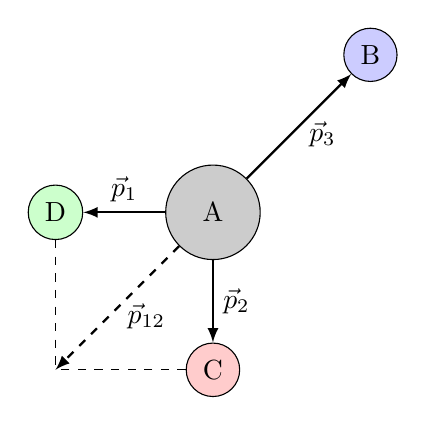
\begin{tikzpicture}
		\node[circle, draw, fill=black!20, minimum size = 1.2cm] (A) at (0,0) {A};
		\node[circle, draw, fill=blue!20] (B) at (2,2) {B};
		\node[circle, draw, fill=red!20] (C) at (0,-2) {C};
		\node[circle, draw, fill=green!20] (D) at (-2,0) {D};

		\draw[-latex, thick] (A)-- node[right, yshift=-0.1cm]{$\vec{p}_3$} (B);
		\draw[-latex, thick] (A)-- node[right]{$\vec{p}_2$} (C);
		\draw[-latex, thick] (A)-- node[above]{$\vec{p}_1$} (D);
		\draw[-latex, dashed, thick] (A) -- node[right, yshift=-0.1cm]{$\vec{p}_{12}$}(-2,-2);
		\draw[dashed] (C) -- (-2,-2);
		\draw[dashed] (D) -- (-2,-2);
	\end{tikzpicture}
	\caption{Schema del decadimento in tre corpi nel sistema del centro di massa}
	\label{fig:decadimento_tre_corpi}
\end{figure}

Nel sistema del centro di massa valgono le seguenti relazioni (la particella
che decade nel sistema del centro di massa ha impulso nullo):
\begin{equation}
	\begin{dcases}
		\vec{p}_1 + \vec{p}_2 + \vec{p}_3 = 0
		\\
		\varepsilon_1 + \varepsilon_2 + \varepsilon_3 = E ^{\ast} = M
	\end{dcases}
	\label{eq:sistema_tre_corpi}
\end{equation}
Per risolvere il problema lo riduciamo in un decadimento in due corpi
introducendo la \textit{particella virtuale}\footnote{
	Il ragionamento può essere applicato a ognuna delle particelle per
	permutazione delle coppie
} $\boldsymbol{DC}$ di massa $M_{12} = m_1 + m_2$, tale che
$M = M _{12} + m_3$, e d'impulso $\vec{p}_{12} = \vec{p}_1 + \vec{p}_2$.
Il quadrimpulso della particella $\boldsymbol{DC}$ sarà la somma dei
quadrimpulsi delle singole particelle:
\begin{equation}
	\qvec{P}_{12}
	= \qvec{P}_1 + \qvec{P}_2
	= \Set{\eps_1 + \eps_2, \vec{p}_1 + \vec{p}_2}
\end{equation}
L'invariante relativistico associato:
\begin{equation}
	M_{12}^2 = \qvec{P}_{12}^2 = \mrb{\eps_1 + \eps_2}^2 -
	\mrb{\vec{p}_1 + \vec{p}_2}^2
\end{equation}
Osserviamo che $M_{12}$ non è costante, ma varia nei limiti cinematici imposti
dalla conservazione del quadrimpulso.
Risolvendo le equazioni \ref{eq:sistema_tre_corpi} per la particella $B$
otteniamo:
\begin{equation}
	M_{12}^2
	= \mrb{M - \eps_3}^2 - \abs{\vec{p}_3}^2
	= M^2 + m_3^2 - 2 M \eps_3
\end{equation}
\begin{equation}
	\Rightarrow \boxed{
		\eps_3 = \frac{M^2 + m_3^2 - M_{12}^2}{2 M}
	}
	\label{eq:epsilon_tre}
\end{equation}
Dall'ultima equazione è evidente come $\eps_3$ dipenda dal valore di
$M_{12}$. Quindi possiamo trovare gli estremi di $\eps_3$, ovvero
$\mrb{\eps_3}_{\text{min}}$ e $\mrb{\eps_3}_{\text{max}}$.

\begin{note}[]
	Possiamo ripetere il ragionamento per per trovare
	$\mrb{\eps_i}_{\text{min,max}}, \forall i = 1, 2, 3$.
\end{note}

\subsection{Energia minima}
La condizione per cui $\eps_3 = \mrb{\eps_3}_{min}$ è che la
particella $\boldsymbol{B}$ sia emessa a riposo rispetto al sistema del centro
di massa\footnote{
	Questa condizione è \textit{cinematicamente ammissibile}
}. Infatti in tale condizione:
\begin{equation}
	\begin{dcases}
		\mrb{\vec{p}_3}_{min} = 0
		\\
		\mrb{\eps_3}_{min} = m_3
	\end{dcases}
\end{equation}
l'energia corrisponde alla massa a riposo (che è l'energia minima che una
particella possa assumere). Dall'equazione \ref{eq:epsilon_tre} otteniamo un
valore per $M_{12}$ in condizione di energia minima per la particella
$\boldsymbol{B}$:
\begin{equation}
	\eps_3 = \frac{M^2 + m_3^2 - M_{12}^2}{2 M} = m_3
\end{equation}
Quindi:
\begin{equation}
	M_{12}^2 =  M^2 + m_3^2 - 2 M m_3 = \mrb{M - m_3}^2
\end{equation}
\begin{equation}
	\Rightarrow \boxed{M_{12} = M - m_3}
\end{equation}
Calcoliamo anche $\abs{\vec{p}\,} = \abs{\vec{p}_1} = \abs{\vec{p}_2}$ relativo
a questa configurazione del sistema:
\begin{equation}
	\begin{dcases}
		\vec{p}_1 + \vec{p}_2 = 0
		\\
		\eps_1 + \eps_2 = M - m_3
	\end{dcases}
\end{equation}
quindi si ricava:
\begin{equation}
	\boxed{
		\abs{\vec{p}}
		= \abs{\vec{p}_1}
		= \abs{\vec{p}_2}
		= \frac{
			\msb{\mrb{M - m_3}^2 - \mrb{m_1 + m_2}^2}
			\msb{\mrb{M - m_3}^2 - \mrb{m_1 - m_2}^2}
		}{4 \mrb{M - m_3}^2}
	}
\end{equation}

\subsection{Energia massima}
Come si può osservare dall'equazione \ref{eq:epsilon_tre}, il valore massimo di
energia $\eps_3$ si ottiene in corrispondenza del valore minimo della
massa invariante $M_{12}$ della particella fittizia $\boldsymbol{DC}$\footnote{
	Sempre in riferimento alla figura \ref{fig:decadimento_tre_corpi}
}.
\begin{equation}
	\mrb{M_{12}}_{\text{min}} \longrightarrow \mrb{\eps_3}_{\text{max}}
\end{equation}
Quindi, scrivendo esplicitamente $M_{12}$:
\begin{align}
	M_{12}^2
	 & = \mrb{\eps_1 + \eps_2}^2 - \mrb{\vec{p}_1 + \vec{p}_2}^2
	\\\notag
	 & = \eps_1^2 + \eps_2^2 + 2 \eps_1 \eps_2 - \abs{\vec{p_1}}^{2} -
	\abs{\vec{p}_{2}}^{2} - 2 \vec{p}_{1} \cdot \vec{p}_{2}
	\\\notag
	 & = m_1^2 + m_2^2 + 2 \mrb{\eps_1 \eps_2 - \vec{p}_1 \cdot
		\vec{p}_2}
\end{align}
quindi, poiché $m_1$ ed $m_2$ sono costanti, $M_{12}$ è minimo quando è minima
la quantità in parentesi. E al minimo la quantità in parentesi vale proprio
$m_1 m_2$. Questa condizione coincide con la configurazione in cui le due
particelle $\boldsymbol{C}$ e $\boldsymbol{D}$ vengono emesse a riposo.
La precedente equazione diventa:
\begin{equation}
	M_{12}^2 \geq \mrb{m_1 + m_2}^2
\end{equation}
e l'uguaglianza \textit{stretta} è rispettata se le due particelle
$\boldsymbol{C}$ e $\boldsymbol{D}$ si muovono nella stessa direzione e con la
stessa velocità, ovvero quando valgono le seguenti condizioni:
\begin{equation}
	\frac{\vec{p}_1}{\eps_1} = \frac{\vec{p}_2}{\eps_2}
	\msse
	\vec{\beta}_1 = \vec{\beta}_2 =\vec{\beta}
\end{equation}

Si verifica, infatti, che sostituendo nell'espressione di $M_{12}^2$
(utilizziamo la relazione $\gamma = \frac{E}{m}$):
\begin{align}
	M_{12}^2
	 & = m_1^2 + m_2^2 + 2 \mrb{\eps_1 \eps_2 - \vec{p}_1 \cdot
		\vec{p}_2}
	\\\notag
	 & = m_1^2 + m_2^2 + 2 \mrb{\eps_1 \eps_2 -
		\beta_1\eps_1 \beta_2\eps_2}
	\\\notag
	 & = m_1^2 + m_2^2 + 2 \eps_1 \eps_2 \mrb{1 - \beta_1 \beta_2}
	\\\notag
	 & = m_1^2 + m_2^2 + 2 \eps_1 \eps_2 \mrb{1 - \beta^2}
	\\\notag
	 & = m_1^2 + m_2^2 + 2 \eps_1 \eps_2 \frac{1}{\gamma^2}
	\\\notag
	 & = m_1^2 + m_2^2 + 2 m_1 \cancel\gamma m_2 \cancel\gamma
	\frac{1}{\cancel\gamma^2}
	\\\notag
	 & = m_1^2 + m_2^2 + 2 m_1 m_2
	\\\notag
	 & = \mrb{m_1 + m_2}^2
\end{align}

Possiamo quindi concludere che:
\begin{equation}
	\boxed{
		\mrb{\eps_3}_{max} = \frac{M^2 + m_3^2 - \mrb{m_1 + m_2}^2}{2M}
	}
\end{equation}

\begin{example}[Decadimento $\beta^-$]
	Vogliamo calcolare l'intervallo di energia permesso all'elettrone nel
	decadimento $\beta^-$ (reazione frequente all'interno dei nuclei atomici):
	\begin{equation}
		n \rightarrow p + e^- + \cc{\nu}_{e}
	\end{equation}
	\textit{Essendo un decadimento a tre corpi, non esiste un'energia ben
		definita per l'elettrone.}
	Le masse delle particelle sono:
	\begin{equation}
		m_n = \qty{939.56}{\MeV \per c^2};
		\qquad
		m_p = \qty{938.27}{\MeV \per c^2};
		\qquad
		m_e = \qty{0.511}{\MeV \per c^2};
		\qquad
		m _{\cc{\nu}} \simeq \qty{0}{\MeV \per c^2}
	\end{equation}
	Quindi le energie per l'elettrone, a reazione avvenuta:
	\begin{equation}
		\begin{dcases}
			\mrb{\eps_{e^-}}_\text{min} = m_{e^-} = \qty{0.511}{\MeV}
			\\
			\mrb{\eps_{e^-}}_\text{max}
			= \frac{m_n^2 + m_{e^-}^2 - m_p^2}{2 m_n}
			\simeq \qty{1.3}{\MeV}
		\end{dcases}
	\end{equation}
\end{example}

\begin{example}[Decadimento del muone]
	Vediamo ora la reazione di decadimento del muone $\mu^+$:
	\begin{equation}
		\mu^+ \rightarrow e^+ + \nu_e + \cc{\nu}_{\mu}
	\end{equation}
	dove $e^+$ è un \textit{positrone}, $\nu_e$ è un \textit{neutrino elettronico}
	e $\cc{\nu}_{\mu}$ un \textit{antineutrino muonico}.
	Le masse sono:
	\begin{equation}
		m _{\mu^+} = \qty{105.7}{\MeV \per c^2};
		\qquad
		m _{\cc{\nu}_{\mu}} = m _{\nu_e} = 0;
		\qquad
		m_{e^+} = \qty{0.511}{\MeV \per c^2}
	\end{equation}
	Quindi le energie:
	\begin{equation}
		\begin{dcases}
			\mrb{\eps_{e^+}}_\text{min} = m_e^+ = \qty{0.511}{\MeV}
			\\
			\mrb{\eps_{e^+}}_\text{max}
			= \frac{m _{\mu}^{2} + \cancel{m_{e^+}^2}}{2 m_{\mu^+}}
			\simeq \frac{m _{\mu^+}}{2}
			= \qty{52.8}{\MeV}
		\end{dcases}
	\end{equation}
\end{example}

\begin{example}[]
	Vediamo un ultimo esempio\footnote{
		La particella $\omega$ è un \textbf{mesone}
	}:
	\begin{equation}
		\omega \rightarrow \pi^+ + \pi^- + \pi^0
	\end{equation}
	Le masse sono:
	\begin{equation}
		m _{\omega} = \SI{782}{\MeV \per c^2};
		\qquad
		m _{\pi} = \SI{140}{\MeV \per c^2}
	\end{equation}
	Le energie:
	\begin{equation}
		\begin{dcases}
			\mrb{\eps _{\pi}}_\text{min} = m _{\pi} = \SI{140}{\MeV}
			\\
			\mrb{\eps _{\pi}}_\text{max} = \frac{m _{\omega}^{2} + m _{\pi}^{2} - 4 m
					_{\pi}^{2}}{2 m _{\omega}} = \frac{m _{\omega}^{2} - 3 m _{\pi}^{2}}{2 m
					_{\omega}} = \SI{353}{\MeV}
		\end{dcases}
	\end{equation}
\end{example}
 % Lezioni 4/5/6 A.A. 2022-2023
% %LTeX: language=it
\chapter{Lezione 31/03/2020}

\section{Metodo delle ellissi - Cambiamento dello spettro di impulsi dal CM al
  Lab}
Trattiamo il problema di una reazione in cui una \textit{particella incide su
	un bersaglio fisso} nel sistema del laboratorio (\textbf{Lab}) note le masse
delle particelle e l'energia della particella incidente.

\begin{note}[]
	D'ora in avanti indicheremo con $p_x, p_y, p_z$ e $p_x^\ast, p_y^\ast,
		p_z^\ast$ rispettivamente le componenti dei vettori $\vec{p}$ e
	$\vec{p}^{\,\ast}$.
\end{note}

\paragraph{Sistema del Centro di Massa}
Nel sistema del centro di massa (\textbf{CM}) sappiamo tutto quello che accade,
perché le particelle finali saranno emesse con impulsi uguali e contrari e le
quantità associate dipenderanno solo dalle masse finali e dalla massa
invariante (ovvero l'energia del centro di massa).
\begin{equation}
	\abs{\vec{p}^{\,\ast}}^{2} = \frac{\msb{M^2 - \mrb{m_1 + m_2}^2} \msb{M^2 -
			\mrb{m_1 - m_2}^2}}{4 M^2}
\end{equation}
\begin{equation}
	\varepsilon_1^\ast = \frac{M^2 + m_1^2 - m_2^2}{2 M};
	\qquad
	\varepsilon_2^\ast = \frac{M^2 + m_2^2 - m_1^2}{2 M}
\end{equation}
Nello spazio degli impulsi possiamo rappresentare i possibili stati della
particella come luogo dei vettori che si muovono su una superficie sferica,
poiché, \textit{in assenza di effetti dinamici}, non c'è motivo di pensare che
ci sia una direzione privilegiata, per cui abbiamo quella che si dice
\textbf{distribuzione angolare isotropa}\footnote{
	Questo per via delle considerazioni puramente cinematiche che stiamo
	effettuando
}.
Questo vuol dire che l'equazione di tale \textit{superficie sferica} sarà data
da:
\begin{align}
	\boxed{\frac{p_x^{\ast 2}}{p^{\ast2}} + \frac{p_y^{\ast2}}{p^{\ast2}} +
	\frac{p_z^{\ast2}}{p^{\ast2}} = 1}
\end{align}

\paragraph{Sistema del Laboratorio}
Nel sistema del centro di massa, come detto, tutto è determinato, ma delle
eventuali misure sperimentali saranno effettuate nel \textit{sistema del
	laboratorio}!

Nel passaggio dal sistema del centro di massa a quello del laboratorio,
supponiamo che la trasformazione di Lorentz avvenga lungo la direzione
$\hat{x}$\footnote{
	È sempre possibile orientare il sistema di riferimento in modo tale che il
	boost di Lorentz avvenga lungo tale direzione
}. Definiamo $\vec{\beta}$ e $\gamma$ rispettivamente la velocità e il
fattore di Lorentz di tale trasformazione. L'\textit{impulso} trasforma nel
seguente modo:
\begin{equation}
	\begin{dcases}
		p_x = \gamma\mrb{p_x^\ast + \beta E^\ast}
		\\
		p_y = p_y^\ast
		\\
		p_z = p_z^\ast
	\end{dcases}
\end{equation}
dove $E^\ast$ è l'energia della particella in oggetto, nel sistema del centro
di massa.

\begin{figure}[ht!]
	\centering
	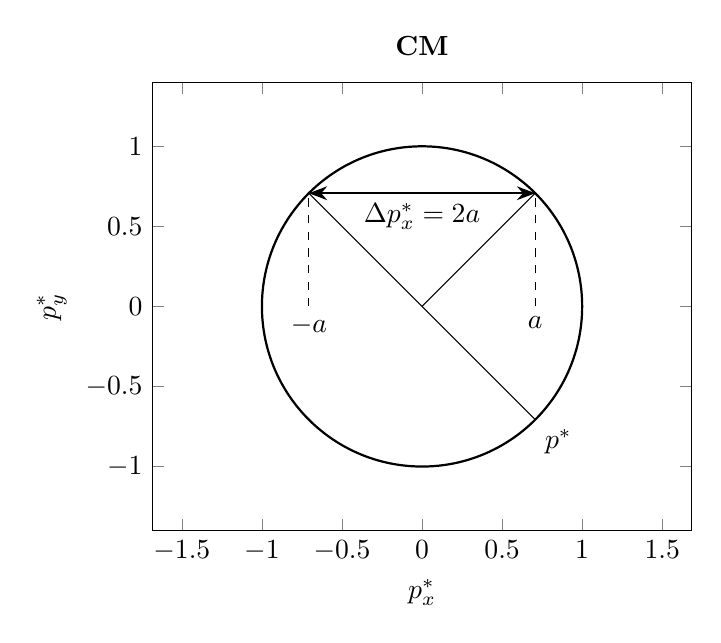
\begin{tikzpicture}
		\tikzset{
			hatch distance/.store in=\hatchdistance,
			hatch distance=10pt,
			hatch thickness/.store in=\hatchthickness,
			hatch thickness=2pt
		}

		\makeatletter
		\pgfdeclarepatternformonly[\hatchdistance,\hatchthickness]{flexible hatch}
		{\pgfqpoint{0pt}{0pt}}
		{\pgfqpoint{\hatchdistance}{\hatchdistance}}
		{\pgfpoint{\hatchdistance-1pt}{\hatchdistance-1pt}}%
		{
			\pgfsetcolor{\tikz@pattern@color}
			\pgfsetlinewidth{\hatchthickness}
			\pgfpathmoveto{\pgfqpoint{0pt}{0pt}}
			\pgfpathlineto{\pgfqpoint{\hatchdistance}{\hatchdistance}}
			\pgfusepath{stroke}
		}
		\begin{axis}[
				title=\textbf{CM},
				xlabel=$p_x^\ast$,
				ylabel=$p_y^\ast$,
				axis equal,
				xmin=-1.2,
				xmax=1.2,
				ymin=-1.4,
				ymax=1.4,
			]

			\draw[
				thick
			] (axis cs:0,0) circle [blue, radius=1];

			\draw[
			] (axis cs:0,0) -- (axis cs:0.707,-0.707)
			node[below right] {$p^\ast$};

			\draw[
			] (axis cs:0,0) -- (axis cs:0.707,0.707);

			\draw[
			] (axis cs:0,0) -- (axis cs:-0.707,0.707);

			\draw[
				Stealth-Stealth,
				thick
			] (axis cs:-0.707,0.707) -- (axis cs:0.707,0.707)
			node[midway, below] {$\Delta p _{x} ^{\ast} = 2a$};

			\draw[
				dashed
			] (axis cs:0.707,0) node[below] {$a$} -- (axis cs:0.707,0.707);

			\draw[
				dashed
			] (axis cs:-0.707,0) node[below] {$-a$} -- (axis cs:-0.707,0.707);
		\end{axis}
	\end{tikzpicture}
	\caption{}
\end{figure}

Consideriamo ora un valore generico $p^\ast_x = a$ tale che $0 < a < p^\ast$;
data la condizione di isotropia, allora possiamo dire che esiste anche un
valore uguale e opposto $p^\ast_x = -a$.
La differenza fra questi due valori sarà $\Delta p_x^\ast = 2a$. Quindi nella
trasformazione per passare al sistema del laboratorio avremo un \textit{boost
	di Lorentz} nella direzione $\hat{x}$, per cui: \begin{equation}
	\begin{dcases}
		\Delta p_x = \gamma \Delta p_x^\ast = \gamma 2a
		\\
		\Delta p_y = \Delta p_y^\ast
		\\
		\Delta p_z = \Delta p_z^\ast
	\end{dcases}
\end{equation}
quindi le altre direzioni, ovviamente, non subiranno boost di Lorentz.

A seguito di tale boost lungo una singola direzione avremo che quella che prima
era una superficie sferica si trasformi in un \textbf{ellissoide} nello spazio
tridimensionale, dove l'asse $x$ è dilatato dal fattore di Lorentz. Tale
ellissoide avrà semiassi:
\begin{align}
	\begin{dcases}
		a_x = \gamma p^\ast
		\\
		a_y = p^\ast
		\\
		a_z = p^\ast
	\end{dcases}
\end{align}

\begin{figure}[ht!]
	\centering
	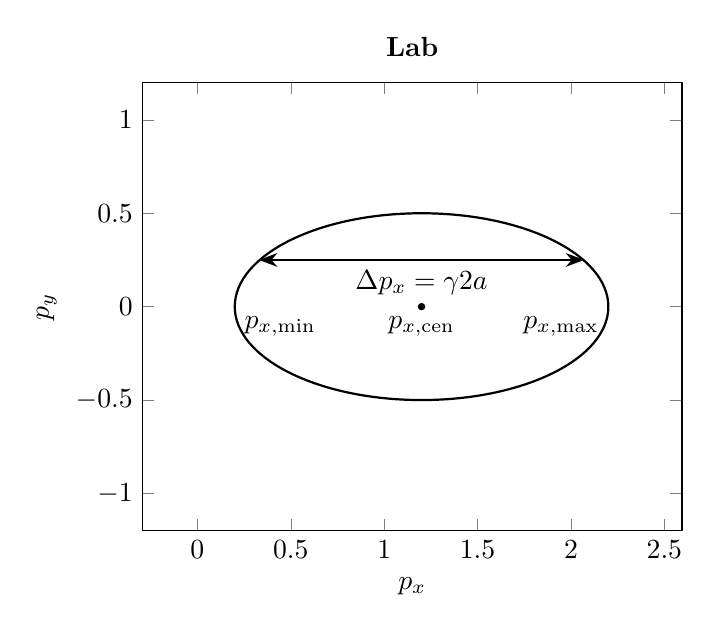
\begin{tikzpicture}
		\begin{axis}[
				title=\textbf{Lab},
				xlabel=$p_x$,
				ylabel=$p_y$,
				axis equal,
				xmin=-0.2,
				xmax=2.5,
				ymin=-1.2,
				ymax=1.2,
			]

			\draw[
				thick
			] (axis cs:1.2,0) ellipse [x radius=1, y radius=0.5];

			\fill[
			] (axis cs:1.2,0) node[below] {$p_{x, \text{cen}}$} circle [radius=0.02];

			\node[below right] at (axis cs:0.2,0) {$p_{x, \text{min}}$};

			\node[below left] at (axis cs:2.2,0) {$p_{x, \text{max}}$};

			\draw[
				Stealth-Stealth,
				thick
			] (axis cs:0.33,0.25) -- (axis cs:2.07,0.25)
			node[midway, below] {$\Delta p _{x} = \gamma 2a$};
		\end{axis}
	\end{tikzpicture}
	\caption{}
\end{figure}

Nello spazio degli impulsi del \textbf{Lab}, il centro dell'ellissoide
coincide al caso $p_x ^{\ast} = 0$, quindi abbiamo:
\begin{equation}
	p_{x}^{\text{cen}} = \beta\gamma E^\ast;
	\qquad
	p_{x}^{\text{min}} = \gamma\mrb{-p^\ast + \beta E^\ast};
	\qquad
	p_{x}^{\text{max}} = \gamma\mrb{p^\ast + \beta E^\ast}
\end{equation}

L'equazione di tale ellissoide\footnote{
	La dipendenza da $E^\ast$ fa sì che l'ellissoide sia diverso per le
	particelle ottenute come prodotto di una certa reazione
}:
\begin{align}
	\textbf{Lab}
	\qquad
	\boxed{
		\frac{\mrb{p_x - \beta \gamma E^\ast}^2}{\gamma^2 p^{\ast\, 2}}
		+ \frac{p_y^2}{p^{\ast2}}
		+ \frac{p_z^2}{p^{\ast2}}
		= 1
	}
\end{align}
La dipendenza dell'ellissoide è dai parametri della trasformazione di Lorentz e
dai parametri della particella particolare presa in considerazione.

Osserviamo che l'ellissoide tocca il piano $p_x = 0$ se:
\begin{equation}
	p_{x}^{\text{min}} = \gamma\mrb{-p^\ast + \beta E^\ast} = 0
\end{equation}
\begin{equation}
	\gamma p^\ast\mrb{- 1 + \frac{\beta E^\ast}{p^\ast}} = 0
	\mthen
	\gamma p^\ast\mrb{\frac{\beta}{\beta^\ast} - 1} = 0
	\msse
	\beta = \beta^\ast
\end{equation}
ovvero se la velocità della trasformazione $\beta$ è uguale alla velocità della
particella nel centro di massa $\beta^\ast = \frac{p^\ast}{E^\ast}$.

Della relazione fra $\beta$ e $\beta^\ast$ possiamo distinguere i tre seguenti
casi:
\begin{itemize}
	\item $\beta < \beta^\ast$: l'ellissoide taglia il piano $p_x$, per cui sono
	      ammessi impulsi tali che $p_x < 0$
	\item $\beta = \beta^\ast$: l'ellissoide è tangente al piano $p_x$, per cui
	      sono ammessi solo impulsi tali che $p_x \geq 0$
	\item $\beta > \beta^\ast$: l'ellissoide è tutto a destra del piano $p_x$ per
	      cui sono ammessi solo impulsi tali che $p_x > 0$
\end{itemize}
 % Lezioni 7/8   A.A. 2022-2023
% %LTeX: language=it
\chapter{Lezione 02/04/2020}
\section{Metodo delle Ellissi (reprise)}
\subsection{Angolo limite nel sistema del Laboratorio}
Per semplicità ma senza perdita di generalità ci poniamo nella condizione $p_z
	= 0$ (con una rotazione attorno all'asse $x$), ovvero riduciamo il problema a
un problema bidimensionale nel piano $\mrb{p_x,p_y}$ nel sistema del
laboratorio e nel corrispondente $\mrb{p_x^\ast,p_y^\ast}$ nel sistema del centro di
massa.

Per il sistema del Laboratorio (\textbf{Lab}) possiamo scrivere:
\begin{equation}
	p_y = p_x \tan \theta
\end{equation}
quindi l'equazione dell'ellisse diventa (nel piano):
\begin{equation}
	\frac{\mrb{p_x - \beta \gamma E^\ast}^2}{\gamma^2 p^{\ast2}}
  + \frac{p_x^2 \tan^2 \theta}{p^{\ast2}}
  = 1
\end{equation}
che, risolvendo rispetto a $p_x$ ha soluzione:
\begin{equation}
	\frac{p_x^2 + \beta^2 \gamma^2 E^{\ast2} - 2 p_x \beta \gamma E^\ast}{\gamma^2 p^\ast}
  + p_x^2 \frac{\tan^2 \theta}{p^{\ast2}}
  - 1
  = 0
\end{equation}
quindi:
\begin{equation}
	p_x^2 \mrb{1 + \gamma^2 \tan^2 \theta}
  + p_x \mrb{-2 \beta \gamma E^\ast}
  + \mrb{\beta^2 \gamma^2 E^{\ast2}
  - \gamma^2 p^{\ast2}}
  = 0
\end{equation}
Le soluzioni:
\begin{equation}
	p_x^\pm = \frac{\beta \gamma E^\ast \pm \sqrt{\mrb{\beta \gamma
				E^\ast}^2 - \mrb{1 + \gamma^2 \tan^2 \theta} \mrb{\beta^2 \gamma^2 E^{\ast2} -
				\gamma^2 p^{\ast2}}}}{1 + \gamma^2 \tan^2 \theta}
\end{equation}
Il discriminante dell'equazione:
\begin{equation}
	\Delta = \mrb{\beta \gamma E^\ast}^2 - \mrb{1 + \gamma^2 \tan^2 \theta}
	\mrb{\beta^2 \gamma^2 E^{\ast2} - 			\gamma^2 p^{\ast2}} = \gamma^2 E^{\ast2}
	\msb{\beta^\ast - \gamma^2 \tan^2 \theta \mrb{\beta^2 - \beta^{\ast2}}}
\end{equation}
e, poiché $\beta^{\ast2} > 0$:
\begin{itemize}
	\item se $\beta < \beta^\ast$, ovvero $\beta^2 - \beta^{\ast2} < 0$, allora il
	      discriminante $\Delta$ sarà positivo e l'equazione ammetterà \textit{due
		      soluzioni} $p_x^\pm$ \textit{reali e distinte}, per qualunque angolo
	      $\theta$;
	\item se $\beta^\ast < \beta$, allora si avrà discriminante positivo, quindi due
	      soluzioni, se e solo se:
	      \begin{equation}
		      \gamma^2 \tan^2 \theta \mrb{\beta^2 - \beta^{\ast2}} \leq \beta^{\ast2}
	      \end{equation}
	      ovvero:
	      \begin{equation}
		      \Rightarrow \tan^2 \theta \leq \frac{\beta^{\ast2}}{\gamma^2 \mrb{\beta^2
				      - \beta^{\ast2}}}
	      \end{equation}
	      Avremo dunque una condizione di \textit{angolo limite} $\theta_{max}$ nel
	      sistema del \textbf{Lab}:
	      \begin{equation}
		      \boxed{
			      \tan^2 \theta_{max}
			      = \frac{\beta^{\ast2}}{\gamma^2 \mrb{\beta^2 - \beta^{\ast 2}}}
		      }
	      \end{equation}
	      e avremo due soluzioni $p_x^\pm$ solo se $\theta < \theta_{max}$. In
	      corrispondenza dell'angolo limite le soluzioni saranno coincidenti e
	      l'impulso considerato è \textit{tangente} all'ellisse.
\end{itemize}

% TODO: figure

\subsection{Angolo limite nel sistema del Centro di Massa}
Possiamo valutare l'angolo $\theta^\ast\mrb{\theta_{max}}$ corrispondente
all'\textit{angolo limite nel sistema del centro di massa} \textbf{CM}.
Effettuando una trasformazione di Lorentz dell'impulso dal sistema del
laboratorio a quello del centro di massa ($\textbf{Lab} \to \textbf{CM}$):
\begin{equation}
	\begin{dcases}
		p_x = \gamma \mrb{p_x^\ast + \beta E^\ast}
		\\
		p_y = p_y^\ast
	\end{dcases}
\end{equation}
quindi:
\begin{equation}
	\tan \theta = \frac{p_y}{p_x} = \frac{p_y^\ast}{\gamma \mrb{p_x^\ast + \beta E^\ast}}
	= \frac{\beta^\ast \sin \theta^\ast}{\gamma \mrb{\beta^\ast \cos \theta^\ast + \beta}}
\end{equation}
Imponendo l'angolo limite:
\begin{subequations}
	\begin{equation}
		\frac{\beta^\ast \sin \theta^\ast\mrb{\theta_{max}}}{\gamma \msb{\beta^\ast \cos
				\theta^\ast\mrb{\theta_{max}} + E^\ast}} = \sqrt{\frac{\beta^{\ast2}}{\gamma^2
				\mrb{\beta^2 - \beta^{\ast2}}}}
	\end{equation}
	\begin{equation}
		\Rightarrow \frac{\cancel{\beta ^{\ast\,2}} \sin ^{2} \theta^\ast
			\mrb{\theta _\text{max}}}{\cancel{\gamma^2} \msb{\beta^\ast \cos
				\theta^\ast \mrb{\theta_\text{max}} + \beta}^{2}} = \frac{\cancel{\beta
				^{\ast\,2}}}{\cancel{\gamma^2} \mrb{\beta^2 - \beta ^{\ast\,2}}}
	\end{equation}
	\begin{equation}
		\Rightarrow \beta^2 \sin ^{2} \theta^\ast \mrb{\theta _\text{max}} - \beta
		^{\ast\,2} \sin ^{2} \theta^\ast \mrb{\theta _\text{max}} = \beta
		^{\ast\,2} \cos ^{2} \theta^\ast \mrb{\theta _\text{max}} + \beta^2 + 2
		\beta \beta^\ast \cos \theta^\ast \mrb{\theta _\text{max}}
	\end{equation}
	\begin{equation}
		\Rightarrow \beta^2 \sin \theta^\ast \mrb{\theta _\text{max}} - \beta
		^{\ast\,2} - \beta^2 - 2 \beta \beta^\ast \cos \theta^\ast \mrb{\theta
			_\text{max}} = 0
	\end{equation}
	\begin{equation}
		\Rightarrow \beta^2 \msb{1 -\cos \theta^\ast \mrb{\theta _\text{max}}} -
		\beta ^{\ast\,2} - \beta^2 - 2 \beta \beta^\ast \cos \theta^\ast
		\mrb{\theta _\text{max}} = 0
	\end{equation}
	\begin{equation}
		\Rightarrow \cancel{\beta^2} - \beta^2 \cos \theta^\ast \mrb{\theta
			_\text{max}} - \beta ^{\ast\,2} - \cancel{\beta^2} - 2 \beta \beta^\ast
		\cos \theta^\ast \mrb{\theta _\text{max}} = 0
	\end{equation}
	\begin{equation}
		\Rightarrow \msb{\beta \cos \theta^\ast \mrb{\theta_\text{max}} +
			\beta^\ast}^{2} = 0
	\end{equation}
\end{subequations}
abbiamo così ottenuto una relazione per l'\textit{angolo $\theta^\ast$ visto dal
	sistema del centro di massa, che corrisponde all'angolo $\theta_{max}$ limite
	visto dal sistema del laboratorio}:
\begin{equation}
	\boxed{\cos \theta^\ast\mrb{\theta_{max}} = -\frac{\beta^\ast}{\beta}}
\end{equation}

\begin{note}[]
	È importare che l'angolo $\theta$ è sempre nell'emisfero sinistro, infatti
	$\cos \theta \leq 0$ ed esiste solo per $\beta > \beta ^{\ast}$.
\end{note}

\begin{example}[Angolo limite]
	Vogliamo studiare il decadimento della particella $\Sigma^+$:
	\begin{equation}
		\pi^+ + p \rightarrow \Sigma^+ + k^+
	\end{equation}
	Le masse delle particelle sono:
	\begin{equation}
		\begin{dcases}
			m _{\pi} = \SI{0.1396}{\GeV \per c^2}
			\\
			m _{p} = \SI{0.9383}{\GeV \per c^2}
			\\
			m _{\Sigma} = \SI{1.189}{\GeV \per c^2}
			\\
			m _{k} = \SI{0.4937}{\GeV \per c^2}
		\end{dcases}
	\end{equation}
	l'impulso iniziale dei pioni è $p _{\pi} = \SI{20}{\GeV \per c}$. Vediamo in
	figura~\ref{fig:rilevatore} uno schema del rivelatore.

	% TODO: figura rilevatore
	Rispondere ai seguenti quesiti:
	\begin{enumerate}
		\item il rilevatore è in grado di vedere tutte le $\Sigma^+$ prodotte (in
		      altri termini: esiste un angolo massimo? e se sì, qual è?)?
		\item le particelle $\Sigma^+$ sono instabili e decadono con un tempo di
		      vita media $\tau_\Sigma = \SI{0.799e-10}{s}$. Assumiamo che tutte le
		      particelle $\Sigma^+$ siano decadute dopo un tempo $3 \tau$; quale deve
		      esser la dimensione $L$ affinché il punto di decadimento sia contenuto
		      nel rivelatore?
		\item calcolare il raggio minimo del rilevatore affinché eso contenga tutti
		      i vertici di decadimento delle $\Sigma^+$;
		\item possiamo vedere tutte le particelle $k^+$?
		\item se così non dovesse essere, quale frazione del numero di particelle
		      $k^+$ che vediamo?
	\end{enumerate}

	\paragraph{Soluzione}
	\begin{enumerate}
		\item \textit{Possiamo vedere tutte le particelle prodotte dalla reazione
			      se l'angolo massimo è $\leq \SI{90}{\degree}$}, considerato come è
		      realizzato il rilevatore. L'energia dei pioni incidenti:
		      \begin{equation}
			      \eps _{\pi} = \sqrt{\abs{\vec{p}_{\pi}}^{2} + m _{\pi}^{2}} \simeq
			      \SI{20}{\GeV}
		      \end{equation}
		      Quindi:
		      \begin{equation}
			      \qvec{P} = \mcb{\eps _{\pi} + m _{p}, \vec{p}_{\pi}}
		      \end{equation}
		      L'\textit{energia del centro di massa}, che \textit{corrisponde alla
			      massa invariante del sistema}:
		      \begin{subequations}
			      \begin{equation}
				      E ^{\ast\,2} = \mrb{\eps _{\pi} + m _{p}}^{2} - \abs{\vec{p}
					      _{\pi}}^{2} = \eps _{\pi}^{2} + m _{p}^{2} + 2 m_p \eps _{\pi} -
				      \abs{\vec{p} _{\pi}}^{2} = m _{p}^{2} + m _{\pi}^{2} + 2 m_p \eps
				      _{\pi}
			      \end{equation}
			      \begin{equation}
				      E^\ast = \sqrt{m _{p}^{2} + m _{\pi}^{2} + 2 m_p \eps _{\pi}} =
				      \SI{6.199}{\GeV}
			      \end{equation}
		      \end{subequations}
		      Il $\beta$ nel centro di massa:
		      \begin{equation}
			      \beta _{\text{CM}} = \frac{\abs{\vec{p}_{\pi}}}{\eps _{\pi} + m _{p}} =
			      0.955187
		      \end{equation}
		      Il $\gamma$ del centro di massa:
		      \begin{equation}
			      \gamma _{\text{CM}} = \frac{\eps _{\pi} + \eps _{p}}{E^\ast} \simeq
			      3.3777
		      \end{equation}
		      L'impulso della particella virtuale che decade a riposo nel sistema del
		      centro di massa:
		      \begin{equation}
			      p^\ast = \frac{\sqrt{\msb{E ^{\ast\,2} - \mrb{m _{\Sigma} + m
								      _{k}}^{2}} \msb{E ^{\ast\,2} - \mrb{m _{\Sigma} - m _{k}}^{2}}}}{2
				      E^\ast} = \SI{2.965}{\GeV \per c}
		      \end{equation}
		      Quindi l'energia nel centro di massa della particella $\Sigma$:
		      \begin{equation}
			      \eps ^{\ast}_{\Sigma} = \sqrt{p ^{\ast\,2} + m^2 _{\Sigma}} \simeq
			      \SI{3.194}{\GeV}
		      \end{equation}
		      allora $\beta ^{\ast}_{\Sigma}$:
		      \begin{equation}
			      \beta ^{\ast}_{\Sigma} = \frac{p^\ast}{\eps ^{\ast}_{\Sigma}} = 0.9283
			      < \beta _{\text{CM}}
		      \end{equation}
		      Questo vuol dire che, per le $\Sigma^+$ \textit{esiste} un angolo limite
		      nel sistema del laboratorio e saremo in grando, dunque, di rilevare
		      \textbf{tutte} le particelle $\Sigma^+$ prodotte.
		      Appurato che esiste un angolo massimo, calcoliamo qual è:
		      \begin{subequations}
			      \begin{equation}
				      \tan \theta _\text{max} = \frac{\beta _{\Sigma}^{\ast}}{\gamma
					      _\text{CM} \sqrt{\beta _\text{CM}^{2} - \beta ^{\ast\,2} _{\Sigma}}}
				      = 1.217
			      \end{equation}
			      \begin{equation}
				      \Rightarrow \theta _\text{max} = \arctan \msb{\frac{\beta
						      _{\Sigma}^{\ast}}{\gamma _\text{CM} \sqrt{\beta _\text{CM}^{2} -
							      \beta ^{\ast\,2} _{\Sigma}}}} = \SI{50.6}{\degree}
			      \end{equation}
		      \end{subequations}
		      questo vuol dire che:
		      \begin{subequations}
			      \begin{equation}
				      \cos \theta^\ast \mrb{\theta _\text{max}} = - \frac{\beta
					      _{\Sigma}^{\ast}}{\beta _\text{CM}} = -0.9717
			      \end{equation}
			      \begin{equation}
				      \Rightarrow \theta^\ast \mrb{\theta _\text{max}} = \SI{166}{\degree}
			      \end{equation}
		      \end{subequations}
		      All'\textit{angolo massimo}, l'\textit{impulso longitudinale}:
		      \begin{equation}
			      \mrb{p _{\Sigma}}_{L} = \gamma _\text{CM} \mrb{p ^{\ast} \cos
				      \theta^\ast \mrb{\theta _\text{max}} + \beta _\text{CM} \eps
				      _{\Sigma}^{\ast}} = \SI{0.573}{\GeV \per c}
		      \end{equation}
		      mentre l'\textit{impulso trasverso}:
		      \begin{equation}
			      \mrb{p _{\Sigma}}_{T} = \mrb{p _{\Sigma}^{\ast}}_{T} = p ^{\ast} \sin
			      \theta^\ast \mrb{\theta _\text{max}} = \SI{0.7}{\GeV \per c}
		      \end{equation}

		\item Rispondiamo alla seconda domanda.
		      \[
			      D _{\Sigma} = 3 \tau _{\Sigma} \gamma _{\Sigma} \beta _{\Sigma} c = 3 c
			      \tau _{\Sigma} \frac{p _{\Sigma}}{m _{\Sigma}} =
			      6.05 \frac{p _{\Sigma}}{\si{\GeV \per c}} \si{\cm}
		      \]
		      L'impulso massimo longitudinale nel sistema del laboratorio:
		      \[
			      \mrb{p _{\Sigma}} _{L, \text{max}} = \gamma _\text{CM} \mrb{p ^{\ast} +
				      \beta _\text{CM} + \eps _{\Sigma}^{\ast}} = \SI{20.3}{\GeV \per c}
		      \]
		      La lunghezza minima per il rilevatore, affinché tutte le particelle
		      $\Sigma$ decadano all'interno del rilevatore:
		      \[
			      L _\text{min} = D _{\Sigma} \mrb{p _{\Sigma}}_{L, \text{max}} =
			      \SI{122.8}{\cm}
		      \]

		\item Rispondiamo al terzo quesito. L'impulso trasverso massimo:
		      \[
			      \mrb{p _{\Sigma}}_{T, \text{max}} = \mrb{p _{\Sigma}^{\ast}}_{T} =
			      p^\ast
		      \]
		      quindi il raggio minimo del rilevatore:
		      \[
			      R _\text{min} = 6.05 \frac{\mrb{p _{\Sigma}}_{T, \text{max}}}{\si{\GeV
					      \per c}} \si{\cm} = \SI{17.9}{\cm}
		      \]

		\item Rispondiamo alla quarta domanda. Sia $m _{k^+}$ la massa della
		      particella
		      $k^+$, con $p ^{\ast} _{k^+}$:
		      \[
			      \eps _{k} = \sqrt{p ^{\ast\, 2} + m _{k}^{2}} = \SI{3.006}{\GeV}
		      \]
		      allora:
		      \[
			      \beta _{k}^{\ast} = \frac{p ^{\ast}}{\eps _{k}^{\ast}} = 0.9864
		      \]
		      quindi $\beta _{k}^{\ast} > \beta _\text{CM}$. Questo vuol dire che
		      alcune particelle verrano emesse all'indietro, quindi non vedremo tutte
		      le particelle emesse.

		\item Rispondiamo alla quinta domanda.
		      \[
			      \mrb{p _{k}^{\ast}}_{L} = p ^{\ast} \cos \theta^\ast \mrb{\SI{90}{\degree}}
			      = - \beta _\text{CM} \eps _{k}^{\ast}
		      \]
		      quindi:
		      \[
			      \cos \theta^\ast \mrb{\SI{90}{\degree}} = - \beta _\text{CM} \frac{\eps
				      _{k}^{\ast}}{p ^{\ast}}
		      \]
		      ricordando che $p^\ast$ è diretto lungo l'asse $y$.
		      Quindi:
		      \[
			      \theta ^{\ast} \mrb{\SI{90}{\degree}} = \SI{165.5}{\degree}
		      \]
		      La porzione visibile di particelle prodotte:
		      \[
			      \tau = \frac{1}{4 \pi} \dint{0}{2 \pi}{\phi}{f}{1}{\cos \theta^\ast}{} = % TODO: controlla qui
			      \frac{1}{2} \mrb{1 - f} = \frac{1.98687}{2} \equiv 98.4 \%
		      \]
	\end{enumerate}
\end{example}
 % Lezioni 8/9   A.A. 2022-2023
% %LTeX: language=it
\chapter{Esercitazione 2022-03-31}
\begin{example}[]
	Fascio di pioni $\pi$ con energia totale $E _{\pi}$ su un bersaglio di
	$\ch{^{2}H}$. Viene prodotta una risonanza:
	\begin{equation}
		M \rightarrow m_1 + m_2
	\end{equation}
	Sapendo che $M = 2.58 m_1$ e che $m_2$ è trascurabile rispetto a $m_1$ ($m_2
		\gg m_1$):
	\begin{enumerate}
		\item Qual è $E _{\pi}$ minima per avere un angolo massimo (\textbf{Lab})
		      per la particella $1$ ($m_1$).
		\item La particella $M$ sarà una particella $\Delta (2420)$ di massa
		      $\qty{2420}{\MeV \per c^2}$.
		      \begin{equation}
			      \Delta (2420) \rightarrow \Sigma + k
		      \end{equation}
		      Le masse sono: $m _{\Sigma} = \qty{1.189}{\GeV \per c^2}$ e $m _{k} =
			      \qty{0.494}{\GeV \per c^2}$.
		      Se la $\Sigma$ viene emessa ad un angolo di $\qty{120}{\degree}$ nel
		      sistema del CM (data l'energia del fascio trovata nel punto $1$) $E
				      _{T} = \qty{2.65}{\GeV}$:
		      \begin{enumerate}
			      \item qual è l'angolo $\theta$ (sistema del laboratorio) che
			            corrisponde all'angolo $\theta^\ast = \qty{120}{\degree}$ nel
			            sistema del centro di massa?
			      \item a quale impulso $p$ (sistema del laboratorio) corrisponde?
		      \end{enumerate}
		\item se un rilevatore lungo \qty{26}{\cm} vede il \qty{99}{\%} dei punti
		      di decadimento della particella $\Sigma$, allora qual è il tempo di
		      vita medio della $\Sigma$?
	\end{enumerate}

	\paragraph{Soluzione}
	\begin{enumerate}
		\item La condizione da soddisfare sarà:
		      \begin{equation}
			      \beta _\text{CM} \geq \beta _{1}^{\ast}
		      \end{equation}
		      L'impulso delle due particelle:
		      \begin{equation}
			      \abs{\vec{p}_{1}^{\,\ast}}
			      = \abs{\vec{p}_{2}^{\,\ast}}
			      = \abs{\vec{p}^{\,\ast}}
			      = \frac{\sqrt{\msb{M^2 - \mrb{m_1 + m_2}^{2}}
					      \msb{M^2 - \mrb{m_1 + m_2}^{2}}}}{2M}
		      \end{equation}
		      L'energia della particella $1$:
		      \begin{equation}
			      \eps _{1}^{\ast} = \frac{M^2 + m_1^2 - m_2^2}{2M}
		      \end{equation}
		      quindi:
		      \begin{equation}
			      p_1^\ast
			      = \frac{p ^{\ast}}{\eps _{1}^{\ast}}
			      = \frac{\sqrt{\mrb{M^2 - m_1^2} \mrb{M^2 - m_1^2}}}{M^2 + m_1^2}
			      = \frac{M^2 - m_1^2}{M^2 + m_1^2}
			      = \frac{2.58^2 - 1}{2.58^2 + 1}
			      = 0.7388
		      \end{equation}
		      Il beta del centro di massa:
		      \begin{equation}
			      \beta _\text{CM}
			      = \frac{\abs{\vec{p} _{\pi}}}{E _{\pi} + m_p}
			      = \frac{\sqrt{E^2 _{\pi} - m _{\pi}^{2}}}{E _{\pi} + m_p}
			      = \beta_1^\ast
		      \end{equation}
		      quindi $E _{\pi}$:
		      \begin{equation}
			      E _{\pi}
			      = \frac{
				      \beta _{1}^{\ast} m_p
				      + \sqrt{\mrb{\beta_1^\ast m_p}^{2}
					      + \mrb{1 - \beta_1^\ast} \mrb{
						      m _{\pi}^{2} + \beta_1 ^{\ast} m_p}
				      }}{1 - \beta_1 ^{\ast\,2}}
			      = \qty{2.65}{\GeV}
		      \end{equation}

		\item Dato che $\theta^\ast = \qty{120}{\degree}$:
		      \begin{equation}
			      \beta _\text{CM} = \beta^\ast_1 = 0.7388
		      \end{equation}
		      \begin{equation}
			      \eps _{\Sigma}^{\ast}
			      = \sqrt{p ^{\ast\, 2} + m _{\Sigma}^{2}}
			      = \qty{1.452}{\GeV}
		      \end{equation}
		      L'impulso $p^\ast$:
		      \begin{equation}
			      p^\ast = \qty{0.833}{\GeV \per c}
		      \end{equation}
		      \begin{equation}
			      \begin{dcases}
				      \mrb{p _{\Sigma}}_{L}
				      = \gamma _\text{CM} \mrb{
					      p ^{\ast} \cos \theta^\ast + \beta _\text{CM} \eps _{\Sigma}^{\ast}
				      }
				      = \qty{0.974}{\GeV \per c}
				      \\
				      \mrb{p _{\Sigma}}_{T}
				      = p^\ast \sin \theta^\ast = \qty{0.721}{\GeV \per c}
			      \end{dcases}
		      \end{equation}
		      Quindi $p _{\Sigma}$:
		      \begin{equation}
			      p _{\Sigma}
			      = \sqrt{\mrb{p _{\Sigma}}_{L}^{2} + \mrb{p _{\Sigma}}_{T}^{2}}
			      = \qty{1.21}{\GeV \per c}
		      \end{equation}
		      L'angolo $\theta _{\Sigma}$ relativo al sistema del laboratorio che
		      stavamo cercando:
		      \begin{equation}
			      \theta _{\Sigma}
			      = \arccos \msb{\frac{\mrb{p _{\Sigma}}_{T}}{p _{\Sigma}}}
			      = \qty{36.5}{\degree}
		      \end{equation}

		\item La distanza media percorsa dalle particelle $\Sigma$ prima del
		      decadimento può essere espresso come:
		      \begin{equation}
			      \braket{L}
			      = c \tau _{\Sigma} \beta _{\Sigma} \gamma _{\Sigma}
			      = c \tau _{\Sigma} \frac{p _{\Sigma}}{m _{\Sigma}}
		      \end{equation}
		      A questo punto, consideriamo:
		      \begin{equation}
			      p _{\Sigma}^\text{max}
			      = \gamma _\text{CM} \mrb{p ^{\ast}
				      + \beta _\text{CM} \eps _{\Sigma}^{\ast}}
			      = \qty{2.83}{\GeV}
		      \end{equation}
		      Il \qty{99}{\%} dgli eventi di decadimento corrisponde a:
		      \begin{equation}
			      \frac{N}{N _\text{tot}} = 0.99
		      \end{equation}
		      e ricordando che il decadimento di particelle è associato a legge
		      esponenziale:
		      \begin{equation}
			      \mint{0}{\infty}{t}{N \mrb{t}}
			      = N _{0} \mint{0}{\infty}{t}{e^{- \frac{t}{\tau _{\Sigma}}}}
			      = N _{0} \tau _{\Sigma}
		      \end{equation}
		      per cui:
		      \begin{equation}
			      0.99
			      = \frac{1}{N _{0} \tau _{\Sigma}} \mint{0}{T}{t}{N \mrb{t}}
			      = \frac{1}{\cancel{N_0} \tau _{\Sigma}}
			      \cancel{N_0} \mint{0}{T}{t}{e^{- \frac{t}{\tau _{\Sigma}}}}
			      = 1 - \mint{T}{\infty}{t}{\frac{1}{\tau _{\Sigma}}
				      e^{- \frac{t}{\tau _{\Sigma}}}}
		      \end{equation}
		      Quindi:
		      \begin{equation}
			      0.99 = 1 - e^{\frac{T}{\tau _{\Sigma}}}
			      \mthen
			      T = - \ln \mrb{0.01} \tau _{\Sigma} = 4.6 \tau _{\Sigma}
		      \end{equation}
		      Ora conosciamo la vita media della particella $\Sigma$, quindi
		      sostituendo nella lunghezza percorsa prima del decadimento:
		      \begin{equation}
			      L
			      = c T \frac{p _{\Sigma}^\text{max}}{m _{\Sigma}}
			      = 4.6 \tau _{\Sigma} \frac{p _{\Sigma}^\text{max}}{m _{\Sigma}}
		      \end{equation}
		      e dunque:
		      \begin{equation}
			      \tau _{\Sigma}
			      = \frac{L m_{\Sigma}}{4.6 c\, p _{\Sigma}^\text{max}}
			      = \frac{0.26 \cdot 1.189}{4.6 \cdot \qty{3e8} \cdot 2.83}\, \si{\s}
			      = \qty{0.79e-10}{\s}
		      \end{equation}
	\end{enumerate}
\end{example}

% %LTeX: language=it
\chapter{2022-04-05}
\begin{example}[]
  Consideriamo un fascio di pioni negativi su una targhetta di protoni:
  \[
    \pi ^{-} + p \rightarrow \Lambda + k^0
  \]
  \begin{enumerate}
    \item Qual è l'energia minima affinché la reazione sia permessa?
    \item assumendo di avere dei pioni di energia $E _{\pi} = \SI{2.0}{\GeV}$,
      stabilire se esiste un angolo massimo (nel sistema del \textbf{Lab}) per
      le particelle $\Lambda$;
  \end{enumerate}

  \paragraph{Soluzione}
  \begin{enumerate}
    \item Le masse delle particelle sono:
      \begin{table}[h!]
        \centering
        \begin{tabular}{r|c}
          \textsc{Pioni} & \SI{140}{\MeV \per c^2}
          \\
          \textsc{Protoni} & \SI{938}{\MeV \per c^2}
          \\
          \textsc{Particella $k$} & \SI{498}{\MeV \per c^2}
          \\
          \textsc{Particella $\Lambda$} & \SI{1116}{\MeV \per c^2}
        \end{tabular}
      \end{table}
      Il quadrimpulso del pione:
      \[
        \qvec{P} _{\pi} = \mcb{E _{\pi}, \vec{p}_{\pi}}
      \]
      mentre il quadrimpulso del protone:
      \[
        \qvec{P}_{p} = \mcb{m _{p}, 0}
      \]
      dato che il protone è la targetta di reazione, che è fissa.
      Il quadrimpulso totale prima della reazione, che fornisce l'informazione
      sull'energia disponibile nel centro di massa:
      \[
        \mrb{\qvec{P}_{\pi} + \qvec{P}_{p}}^{2} = E _{\pi}^{2} + m _{p}^{2} + m
        m_p E _{\pi} - \abs{\vec{p}_{\pi}}^{2} = m _{\pi}^{2} + m _{p}^{2} + 2
        m_p E _{\pi}
      \]
      Quindi avremo:
      \[
        m _{\pi}^{2} + m _{p}^{2} + 2 m_p E _{\pi} = \mrb{m _{\Lambda} + m
        _{k}}^{2}
      \]
      Dobbiamo determinare l'energia minima dei pioni incidenti, per cui
      invertiamo la relazione:
      \[
        E _{\pi} = \frac{\mrb{m _{\Lambda} + m _{k}}^{2} - m _{\pi}^{2} - m
        _{p}^{2}}{2 m_p} = \SI{0.91}{\GeV}
      \]

    \item Dobbiamo determinare se vale la seguente relazione: $\beta^\ast
      _{\Lambda} < \beta _\text{CM}$.
      \[
        \beta _\text{CM} = \frac{\abs{\vec{p}\,}}{E} = \SI{0.68}{}
      \]
      L'energia disponibile del centro di massa:
      \[
        E ^{\ast} = \sqrt{\mrb{\qvec{P}_{\pi} + \qvec{P}_{p}}^{2}} = \sqrt{m
        _{p}^{2} + m _{\pi}^{2} + 2 E _{\pi} m _{p}} = \SI{2.16}{\GeV}
      \]
      A questo punto possiamo calcolare:
      \[
        \abs{\vec{p}_{k}^{\ast}} = \abs{\vec{p}_{\Lambda}^{\ast}} =
        \abs{\vec{p}^{\ast}} = \frac{\sqrt{\msb{E ^{\ast\,2} - \mrb{m
        _{\Lambda} + m_k}^{2}} \msb{E ^{\ast\,2} - \mrb{m _{\Lambda} - m
        _{k}}^{2}}}}{2 E^\ast}
      \]
      Quindi:
      \[
        \beta _{\Lambda}^{\ast} = \frac{p ^{\ast}}{\sqrt{p ^{\ast\, 2} + m
        _{\Lambda}^{2}}} = 0.52
      \]
      Quindi \textit{esiste} un angolo massimo e dunque $\beta _{L}^{\ast} <
      \beta _\text{CM}$ e tale angolo vale:
      \[
        \theta _\text{max} = \arctan \mcb{\msb{\gamma _\text{CM}
        \sqrt{\mrb{\frac{\beta _\text{CM}}{\beta ^{\ast}_{\Lambda}}}^{2} -
        1}}^{-1}} = \SI{0.73}{\radian} \simeq \SI{42}{\degree}
      \]
  \end{enumerate}
\end{example}

\begin{example}[]
  Consideriamo due fasci di particelle che collidono in un \textit{collider}.
  Sia il primo fascio di particelle un fascio di $e^-$ e sia la rispettiva
  energia $E _{1} = \SI{12}{\GeV}$; sia il secondo fascio di particelle un
  fascio di $e^+$ e sia la rispettiva energia $E _{2} = \SI{5}{\GeV}$.
  Determinare:
  \begin{enumerate}
    \item l'energia totale nel centro di massa;
    \item l'impulso degli elettroni nel sistema del centro di massa;
    \item $\beta _\text{CM}$ e $\gamma _\text{CM}$.
  \end{enumerate}

  \paragraph{Soluzione}
  \begin{enumerate}
    \item L'energia disponibile nel centro di massa sarà:
      \begin{align*}
        E ^{\ast\,2} &= \mrb{\qvec{P}_{1} + \qvec{P}_{2}} = \mrb{E_1 + E_2} ^{2}
        - \mrb{\vec{p}_{1} + \vec{p}_{2}}^{2}
        \\
        &= E_1^2 + E_2^2 + 2 E_1 E_2 -
        \abs{\vec{p}_{1}}^{2} - \abs{\vec{p}_{2}}^{2} + 2 \abs{\vec{p}_{1}}
        \abs{\vec{p}_{2}}
        \\
        &= \sqrt{2 m_e^2 + 2 E_1 E_2 + 2 \abs{\vec{p}_{1}} \abs{\vec{p}_{2}}}
      \end{align*}
      Ora, considerando che le energie $E_{1,2}$ sono molto maggiori delle
      masse degli elettroni, possiamo considerare la seguente approssimazione:
      \[
        E ^{\ast} \simeq \sqrt{2 E_1 E_2 + 2 E_1 E_2} = \sqrt{4 E_1 E_2} = 2
        \sqrt{E_1 E_2} = \SI{15.5}{\GeV}
      \]

    \item Nel sistema del centro di massa possiamo considerare che i due fasci
      abbiano lo stesso impulso e quindi che si spartiscano l'energia
      disponibile nel centro di massa:
      \[
        p ^{\ast} = \frac{E ^{\ast}}{2}
      \]

    \item Calcoliamo i valori richiesti.
      \[
        \beta _\text{CM} = \frac{\abs{\vec{p}_{1} + \vec{p}_{2}}}{E_1 + E_2} =
        \frac{\sqrt{E_1^2 - m_e^2} - \sqrt{E_2^2 - m_e^2}}{E_1 + E_2}
      \]
      a questo punto possiamo fare l'approssimazione di trascurare le masse
      rispetto alle energie:
      \[
        \beta _\text{CM} = \frac{E_1 - E_2}{E_1 + E_2} = 0.4
      \]

      Il $\gamma _\text{CM}$, invece:
      \[
        \gamma _\text{CM} = \frac{1}{\sqrt{1 - \beta _\text{CM}^{2}}} = 1.1
      \]
  \end{enumerate}
\end{example}

\begin{example}[Ultra High Cosmic Rays]
  Consideriamo il processo di \textit{Photo-Pion production}:
  \[
    p + \gamma _\text{CMB} \rightarrow p + \pi^0
  \]
  dove $\gamma _\text{CMB}$ rappresenta un fotone delle \textsc{Cosmic
  Microwave Background} (o \textit{Radiazione Cosmica di Fondo}).
  I dati del problema sono:
  \begin{table}[h!]
    \centering
    \begin{tabular}{r|c}
      Massa dei Protoni & $M_p = \SI{0.94}{\GeV \per c^2}$
      \\
      Massa dei Pioni & $M _{\pi} = \SI{140}{\MeV \per c^2}$
      \\
      Energia dei fotoni della radiazione & $E _{\gamma _\text{CMB}} =
      \SI{e-3}{\eV}$
      \\
      Energia dei raggi cosmici (protoni) & $E _\text{CR} > \SI{e18}{\eV}$
    \end{tabular}
  \end{table}

  \begin{enumerate}
    \item Studiare la dipendenza della soglia in energia in funzione
      dell'angolo di scattering;
    \item calcolare l'energia minima.
  \end{enumerate}

  \paragraph{Soluzione}
  \begin{enumerate}
    \item Calcoliamo i quadrimpulsi:
      \[
        \qvec{P}_{p} = \mcb{E _{p}, \vec{p}_{p}}
        \qquad
        \qvec{P}_{\gamma _\text{CMB}} = \mcb{E _{\gamma _{\text{CMB}}},
        \vec{p}_{\gamma _\text{CMB}}}
      \]
      Per semplificare indichiamo con $\gamma$ le particelle $\gamma
      _\text{CMB}$, quindi, ricordando che $\gamma$ sono fotoni e sono quindi
      \textit{massless}:
      \[
        E _{p}^{2} + \cancel{E _{\gamma}^{2}} + 2 E _{p} E _{\gamma} - p
        _{p}^{2} - \cancel{p _{\gamma}^{2}} - 2 \vec{p}_{p} \cdot
        \vec{p}_{\gamma} = \mrb{M _{p} + M _{\pi}}^{2}
      \]
      Considerato che $E _{p} \sim \SI{e18}{\eV}$, possiamo procedere con
      l'approssimazione $E _{p} \simeq p _{p}$, inoltre possiamo sostituire
      $\vec{p}_p \cdot \vec{p}_{\gamma} = E _{p} E _{\gamma} \cos \theta$, dove
      $\theta$ è l'\textit{angolo di scattering}. Dunque:
      \[
        2 E_p E _{\gamma} + M _{p}^{2} - E _{p} E _{\gamma} \cos \theta =
        \mrb{M _{p} + M _{\pi}}^{2}
      \]
      L'energia di soglia (\textit{threshold}):
      \[
        E _{p} ^\text{th} = \frac{\mrb{M_p + M _{\pi}}^{2} - M _{p}^{2}}{2 E
        _{\gamma} \mrb{1 - \cos \theta}}
      \]

    \item Il minimo sull'energia si ottiene quando $\theta = \pi$, ovvero per
      urto frontale. Quindi l'energia minima di soglia sarà:
      \[
        E _\text{min}^\text{th} = \frac{\mrb{M _{p} + M _{\pi}}^{2} - M _p
        ^{2}}{4 E _{\gamma}} = \SI{6.8e19}{\eV}
      \]
  \end{enumerate}
\end{example}

\begin{example}[UHECR]
  Consideriamo di nuovo un processo che coinvolge \textsc{Ultra High Energy
  Cosmic Rays}.
  \[
    p + \gamma _\text{CMB} \rightarrow p + e^+ + e^-
  \]

  \[
    \qvec{P}_{p} = \mcb{E _{p}, \vec{p}_{p}}
    \qquad
    \qvec{P}_{\gamma} = \mcb{E _{\gamma}, \vec{p}_{\gamma}}
  \]
  quindi:
  \[
    E^2 _{p} + \cancel{E _{\gamma}^{2}} + 2 E _{p} E _{\gamma} - p^2 _{p} +
    \cancel{p ^{2} _{\gamma}} - 2 \vec{p}_{p} \cdot \vec{p}_{\gamma} = \mrb{M
    _{p} + 2 m_e}^{2}
  \]
  Sfruttando l'approssimazione $m _{e} \ll M _{p}$:
  \[
    \Rightarrow 2 E_p E _{\gamma} \mrb{1 - \cos \theta} = \mrb{M _{p} + 2
    m_e}^{2} - M _{p}^{2} = \cancel{M _{p}^{2}} + 4 m _{e}^{2} + 4 M _{p} m_e -
    \cancel{M _{p}^{2}} \simeq 4 M_p m_e
  \]
  quindi:
  \[
    E ^\text{th} \mrb{\theta} = \frac{2 m_e M_p}{E _{\gamma_\text{CMB}} \mrb{1
    - \cos \theta}}
  \]
  Quindi il minimo dell'energia di soglia, che si ha per $\theta = \pi$:
  \[
    E ^\text{th}_\text{min} = \frac{m_e M _{p}}{E _{\gamma _\text{CMB}}} =
    \SI{0.5e18}{\eV}
  \]
\end{example}

\begin{note}[]
  Sulle dispense del professore ci sono ulteriori $2$ esercizi svolti.
\end{note}


\part{Fisica Nucleare - Prof. Villante/Capozzi}
%LTeX: language=it
\chapter{2023-04-27}
\section{Serie (catene) radiattive}
Furono individuate $3$ \textit{serie} (catene) \textit{radiattive}:

Le catene radiattive sono originate da tre tipi di decadimento:
\begin{itemize}
	\item $\alpha$ \rightarrow \textit{particelle cariche} $\ch{^{4}He^{++}}$;
	\item $\beta$ \rightarrow \textit{particelle negative};
	\item $\gamma$ \rightarrow \textit{particelle neutre} (fotoni energetici).
\end{itemize}
I primi e maggiori sviluppi in fisica nucleare sono stati fatti utilizzando
particelle $\alpha$.

\section{Rutherford scattering formula}
Utilizzeremo particelle con carica $ze$.

\subsection{Il modello}
\begin{itemize}
	\item L'atomo è costituito da un nucleo con carica positiva $Ze$ che porta
	      praticamente tutta la massa dell'atomo;
	\item l'atomo è elettricamente neutro e contiene $Z$ elettroni che orbitano
	      intorno al nucleo. Questi elettroni non possono dar luogo a deflessioni
	      grandi. Sono trascurabili rispetto alla particella $\alpha$, considerata
	      come proiettile;
	\item il nucleo bersaglio è molto più massivo della particella incidente;
	      questo permetterà in prima approssimazione di considerare il rinculo del
	      target nullo, $m \ll M$;
	\item si utilizza solo meccanica classica per descrivere l'urto, quindi
	      assumeremo la velocità del proiettile non relativistica, $v \ll c$;
	\item il nucleo bersaglio e la particella incidente hanno distribuzioni di
	      carica puntiforme e interagiscono attraverso un potenziale coulombiano
	      (interazione puramente elettromagnetica):
	      \begin{equation}
		      V \mrb{z} = \frac{Z z e^2}{4 \pi \eps_0 r}
	      \end{equation}
	\item si considera l'interazione elettromagnetica come unico tipo
	      d'interazione;
	\item il bersaglio e il proiettile non subiscono alcuna eccitazione durante
	      l'urto (scattering elastico).
\end{itemize}


La forza d'interazione del modello è la forza coulombiana:
\begin{equation}
  \vec{F} = \frac{z Z e^2}{4 \pi \eps_0} \frac{\hat{r}}{r^2}
\end{equation}
L'impulso trasferito, se gli impulsi iniziale e finale della particella prima e
dopo l'urto sono $\vec{p}_{i}$ e $\vec{p}_{f}$ rispettivamente:
\begin{equation}
  \Delta \vec{p} = \abs{\vec{p}_{f} - \vec{p}_{i}} = 2 p \sin \frac{\theta}{2}
\end{equation}
allora:
\begin{equation}
  \Delta p = \int_{-\infty}^{\infty} F_T \md[]{t}
  = \int_{-\infty}^{\infty} \frac{z Z e^2}{4 \pi \eps_0} \frac{cos \beta}{r^2} \md[]{t}
\end{equation}
dove, con $\beta$ l'angolo in figura \ref{fig:rutherford_scattering}:
\begin{equation}
  \beta \mrb{t = - \infty} = - \mrb{\frac{\pi}{2} - \frac{\theta}{2}};
  \qquad
  \beta \mrb{t = \infty} = \frac{\pi}{2} - \frac{\theta}{2}
\end{equation}

\subsection{Raggio di collisione}
\begin{equation}
  \tan \frac{\theta}{2}
  = \frac{z Z e^2}{4 \pi \eps_0 b} \frac{m}{p^2}
  = \frac{R}{b}
\end{equation}
con $R = \frac{z Z e^2 m}{4 \pi \eps_0 p^2}$.
In particolare, per $R = b$ abbiamo:
\begin{equation}
  \tan \frac{\theta}{2} = 1
  \mthen
  \frac{\theta}{2} = \qty{45}{\degree}
  \mthen \theta = \qty{90}{\degree}
\end{equation}

Per il caso di impatto frontale, utilizziamo il \textit{teorema delle forze
vive}:
\begin{equation}
  T + V = \text{const}
\end{equation}
quindi:
\begin{equation}
  \frac{1}{2} m v_0^2 + 0
  = \text{const}
  = 0 + \frac{z Z e^2}{4 \pi \eps_0 r_{\text{min}}}
\end{equation}
allora abbiamo che:
\begin{equation}
  r_{\text{min}} = 2 R
\end{equation}
Questo vuol dire che L'ordine di grandezza di $R$ rappresenta l'ordine di
grandezza della minima distanza della particella $\alpha$ dal nucleo
scatteratore.

%LTeX: language=it
\chapter{2020-02-27} % 2020-02-27
\section{Grandezze atomiche caratteristiche}
\begin{table}[h!]
  \centering
  \caption{Caratteristiche degli elettroni}
  \begin{tabular}{r|c}
    \textbf{Raggio atomo} & $R_A = 1\si{\angstrom} =
    \SI{e-10}{\m} = \SI{e-8}{\cm}$
    \\
    \textbf{Energie} & $E \sim \SI{1}{\eV}$
    \\
    \textbf{Massa elettrone} & $m_e \simeq \SI{9e-31}{\kg}$
    \\
    \textbf{Energia riposo elettrone} & $m_ec^2 \simeq \SI{0.511}{\MeV}$
  \end{tabular}
\end{table}

\begin{table}[h!]
  \centering
  \caption{Caratteristiche dei nuclei}
  \begin{tabular}{r|c}
    \textbf{Raggio nucleo} & $R_N = \SI{e-15}{\m} =
    \SI{e-13}{\cm} = \SI{1}{\femto\m}$
    \\
    \textbf{Massa protone} & $m_p \simeq 1836 m_e$
    \\
    \textbf{Energia riposo protone} & $m_pc^2 \simeq \SI{1}{\GeV}$
    \\
    \textbf{Energia riposo neutrone} & $m_nc^2 \simeq m_pc^2$
    \\
    \textbf{Energie} & $E \sim \SI{1}{\keV} \div \SI{1}{\MeV}$
  \end{tabular}
\end{table}
Poiché le masse di protone e neutrone risultano molto simili (la differenza fra
le energie a riposo\\ $m_nc^2 - m_pc^2 \simeq 1.29\si{\MeV}$), capiterà di
lavorare con la \textbf{massa del nucleone} (che indicheremo con la N
maiuscola) e la rispettiva energia a riposo: $m_Nc^2 \simeq 1\si{\GeV}$.\par
La fisica nucleare si può studiare trascurando l'influenza degli elettroni.

\section{Grandezze Caratteristiche - Indeterminazione di Heisenberg}
A causa del \textit{Principio di Indeterminazione di Heisenberg} lo studio di
fenomeni che avvengono a distanze molto piccole è possibile solo se abbiamo a
che fare con energie molto grandi.
\begin{equation}
  \Delta x \Delta p_x \gtrsim \hbar
\end{equation}
Immaginiamo il nucleo come un come un contenitore (consideriamo per ora la
direzione $\hat{x}$, ma varranno le stesse considerazioni anche per le
direzioni $\hat{y}$ e $\hat{z}$) di dimensione caratteristica $R_N$. Se
assumiamo una particella localizzata all'interno di tale contenitore, per il
principio di Heisenberg si avrà $\Delta x = R_N$. Inoltre, poiché non c'è
motivo di pensare che ci sia un verso privilegiato, possiamo dire per l'impulso
$p_x$ che $\braket{p_x} = \overline{p_x} = 0$.\par
Allora:
\begin{equation}
  \left(\Delta p_x\right)^2 = \braket{\left(p_x - \overline{p_x}\right)^2} =
  \braket{p_x^2 - 2p_x\overline{p_x} + \overline{p_x}^2} = \braket{p_x^2}
  \label{eq:deltap_x}
\end{equation}
Inoltre, $\Delta p_x$ ammetterà un limite inferiore avendo definito $\Delta x$,
ovvero:
\begin{equation}
  \Delta p_x \gtrsim \frac{\hbar}{\Delta x} = \frac{\hbar}{R_N}
\end{equation}
per cui, utilizzando l'equazione \ref{eq:deltap_x}:
\begin{equation}
  \left(\Delta p_x\right)^2 = \braket{p_x^2} \gtrsim
  \left(\frac{\hbar}{R_N}\right)^2
\end{equation}
Analogamente si può ripetere il ragionamento anche per le altre direzioni:
\begin{equation}
  \braket{p_x^2} \gtrsim \left(\frac{\hbar}{R_N}\right)^2
  \qquad
  \braket{p_y^2} \gtrsim \left(\frac{\hbar}{R_N}\right)^2
  \qquad
  \braket{p_z^2} \gtrsim \left(\frac{\hbar}{R_N}\right)^2
  \label{eq:impulso_quadro_medio}
\end{equation}
Considerando energie \textit{NON-relativistiche}, definiamo l'energia cinetica
come energia cinetica classica:
\begin{equation}
  K = \frac{\abs{\vec{p}\,}^2}{2m} = \frac{p_x^2 + p_y^2 + p_z^2}{2m}
\end{equation}
e sfruttando il set di equazioni \ref{eq:impulso_quadro_medio} possiamo
stabilire un \textbf{limite inferiore
per l'energia cinetica media} (sempre conseguenza del principio di
Indeterminazione):
\begin{equation}
  \braket{K} = \frac{\braket{p_x^2} + \braket{p_y^2} + \braket{p_z^2}}{2m}
  \gtrsim \frac{3}{2m_N} \left(\frac{\hbar}{R_N}\right)^2
\end{equation}

\paragraph{Stime}
Per avere un'idea degli ordini di grandezza delle quantità con cui avremo a che
fare possiamo moltiplicare e
dividere per $c^2$, per cui\footnote{
  Una quantità molto utile per i conti sarà $\hbar c \simeq \SI{197}{\MeV
  \femto\m}$
}, per un \textit{nucleo}:
\begin{equation}
  \braket{K} \gtrsim \frac{3}{2}\frac{(\hbar c)^2}{(m_N c)^2}\frac{1}{R_N^2} =
  \frac{3}{2}\frac{(200)^2}{1000}
  \frac{\si{\MeV}}{\left(\nicefrac{R_N}{1\si{\femto\m}}\right)^2} =
  \frac{60\si{\MeV}} {\left(\nicefrac{R_N}{1\si{\femto\m}}\right)^2}
\end{equation}

Lo stesso conto, per un \textit{atomo}:
\begin{equation}
  \braket{K} = \frac{3}{2} \frac{1}{m_e c^2} \frac{\mrb{\SI{200}{\MeV
  \femto\m}}^{2}}{R_\text{atomo}^{2}} \simeq \SI{e-5}{\MeV} = \SI{10}{\eV}
\end{equation}

\begin{note}[]
  Al bilancio energetico bisognerà aggiungere un \textbf{termine di repulsione
  coulombiana} ed uno di attrazione dell'\textbf{interazione forte fra
  nucleoni}.
\end{note}

\begin{note}[Potenziale Coulombiano]
  Vediamo qualche dettaglio sulle dimensioni del potenziale di interazione
  coulombiana in modulo (quindi che sia attrattivo o repulsivo):
  \begin{equation}
    \abs{V_\text{coulomb}} = \frac{e^2}{4 \pi \eps_0} \frac{1}{R} =
    \frac{e^2}{4 \pi \eps_0} \frac{\hbar c}{\hbar c} \frac{1}{R} = \alpha
    \frac{\hbar c}{R} \simeq \frac{200}{137} \frac{1}{\si{R \per \femto\m}}
    \si{\MeV}
  \end{equation}
  dato che $\frac{e^2}{4 \pi \eps_0 \mrb{\hbar c}} = \alpha \simeq
  \frac{1}{137}$.
\end{note}

\section{Esperimenti di Rutherford}
\label{sec:rutherford}
Gli esperimenti di Rutherford che illustriamo erano volti a scoprire alcune
proprietà dei nuclei fra cui le dimensioni e consistevano in quelli che
definiamo \textbf{scattering nucleari di particelle} $\boldsymbol{\alpha}$.\par
Particelle $\alpha$ (nuclei di elio \ch{He^4}) venivano collimate su una lamina
molto sottile \footnote{
  Si trattava di circa $\SI{4}{\mu\m}$ perché si sperava di osservare
  l'effetto di \textbf{singola interazione}
} di oro (per evitare scattering multipli) e venivano poi osservate
da dei rilevatori che ne misuravano l'angolo di deflessione.

\subsection{Descrizione Classica}
Consideriamo un'interazione \textit{particella $\alpha$/nucleo}\footnote{
  Stiamo parlando quindi della propagazione di una particella carica in un
  campo elettrostatico fisso nello spazio e nel tempo: in questa configurazione
  la quantità di moto della particella non è una quantità conservata, poiché il
  campo elettrostatico fisso rompe l'invarianza per traslazione
} di tipo
\text{coulombiano} e \textbf{trascuriamo il rinculo del nucleo}, ovvero
fissiamo le ipotesi:
\begin{equation}
  m_N \gg m_\alpha \qquad m_Nc^2 \gg K
\end{equation}

\begin{figure}[ht]
  \centering
  \begin{tikzpicture}
    \draw[dashed] (-4,0) -- (6,0);
    \draw[dashed] (-4,2) -- (6,2);
    \draw[semithick, color=purple] (0,0) arc [radius=1.5, start angle=180, end angle=158.5] (0,0) node[below]{$\beta$};
    \draw[semithick, color=purple] (-2,2) arc [radius=1.5, start angle=0, end angle=-22.8] (-2,2) node[above]{$\beta$};
    \draw[-latex] (1.5,0) -- (-3.45,1.95) node[below]{$\vec{r}$};
    \draw[latex-latex, thick] (5,0) -- (5,2);
    \draw (5,1) node[right]{$b$};

    \draw[dashed] (1.5,0) -- (6,4.5);
    \draw[dashed] (0.672,2) -- (4.086,5.414);
    \draw[-latex, dashed] (1.5,0) -- (0.672,2);
    % \draw[dashed] (1.5,0) -- (1.5,5);

    \draw[latex-latex, thick] (5.5,4) -- (4.086,5.414);
    \draw (4.793,4.707) node[right, yshift=0.1cm]{$b$};

    \draw[semithick] (2.5,0) arc [radius=1, start angle=0, end angle=45] (2.5,0) node[below]{$\theta$};
    \draw[semithick] (1.672,2) arc [radius=1, start angle=0, end angle=45] (1.672,2) node[below]{$\theta$};

    \filldraw[color=blue] (-3.5,2) circle (2pt) node[above]{$\alpha, ze$};
    \draw[-latex, thick, color=blue] (-3.5,2) -- (-2.5,2) node[above]{$\vec{v}_i$};
    \filldraw[color=red] (1.5,0) circle (3pt) node[below]{$N, Ze$};
    \filldraw[color=blue] (1.5,2.832) circle (2pt);
    \draw[-latex, thick, color=blue] (1.5,2.832) -- (1.5+0.707,2.832+0.707) node[right, yshift=-0.1cm]{$\vec{v}_f$};
  \end{tikzpicture}
  \caption{$b$: \textit{\textbf{parametro d'impatto}}; $\vec{v}_i$:
  \textit{velocità iniziale}; $\vec{v}_f$: \textit{velocità finale}}
  \label{fig:rutherford_scattering}
\end{figure}

Nell'ipotesi in cui il \textit{nucleo non rinculi} avremo per i principi di
conservazione che $\abs{\vec{v}_f} = \abs{\vec{v}_i}$, ossia che l'energia
cinetica della particella incidente sia invariata dopo lo scattering.
indicheremo con $\theta$ il cosiddetto \textbf{angolo di scattering}, ovvero
l'angolo fra le direzioni associate a $\vec{v}_{i}$ e $\vec{v}_{f}$.
Analizziamo ora i due casi di scattering per parametro d'urto $b=0$ e $b\neq0$.
\begin{itemize}
  \item Caso $\boxed{\boldsymbol{b = 0} \Rightarrow \theta =
    180\si{\degree}}$\\
    Possiamo calcolare la \textbf{distanza di massimo avvicinamento} come:
    poiché siamo in descrizione classica scriviamo l'energia totale del sistema
    come l'energia cinetica classica della particella $\alpha$, più il
    potenziale coulombiano di interazione fra particella e nucleo:
    \begin{equation}
      E_T = \frac{1}{2}m_\alpha \abs{\vec{v}\,}^2 + \frac{zZe^2}{4\pi\epsilon_0
      \abs{\vec{r}\,}} = \text{const}
    \end{equation}
    Tramite una semplice considerazione sulla \textbf{conservazione
    dell'energia totale} del sistema (ricorda che siamo in fisica classica)
    possiamo scrivere uguagliando l'energia totale iniziale (che supponendo la
    particella $\alpha$ a distanza infinita dal nucleo sarà composta del solo
    termine cinetico) e l'energia totale al punto di inversione del moto (che
    sarà composta del solo termine potenziale poiché al punto di inversione
    $\abs{\vec{v}\,} = 0$),
    quindi:
    \begin{equation}
      \frac{1}{2}m_\alpha \abs{\vec{v}_i}^2 =
      \frac{zZe^2}{4\pi\epsilon_0}\frac{1}{\rho}
      \label{eq:cons_en_rutherford}
    \end{equation}
    Dove abbiamo chiamato $\rho$ la \textbf{distanza di massimo
    avvicinamento per urto frontale}.

    Invertendo l'equazione \ref{eq:cons_en_rutherford} otteniamo:
    \begin{equation}
      \rho = \frac{zZe^2}{4\pi\epsilon_0}\frac{2}{m\abs{\vec{v}_i}^2} =
      \frac{zZe^2}{4\pi\epsilon_0}\frac{\hbar c}{\hbar
      c}\frac{2}{m\abs{\vec{v}_i}^2}
    \end{equation}
    Dove l'ultimo passaggio ci permette di esprimere $\rho$ in termini di
    costante di struttura fine:
    \begin{equation}
      \textbf{Costante di struttura fine}
      \qquad
      \boxed{
        \alpha = \frac{e^2}{4\pi\epsilon_0}\frac{1}{\hbar c} \simeq
        \frac{1}{137}
      }
    \end{equation}
    Quindi infine la \textbf{distanza di massimo avvicinamento per urto
    frontale} diventa:
    \begin{equation}
      \boxed{
        \rho = zZ\alpha\frac{\hbar c}{\frac{m\abs{\vec{v_i}}^2}{2}} =
        zZ\alpha\frac{\hbar c}{K}
      }
      \label{eq:dist_max_avvicinamento}
    \end{equation}

    \paragraph{Stime} Ricordando che il raggio atomico è dell'ordine del
    \text{fermi}, possiamo osservare da una stima grossolana che (secondo la
    descrizione classica) per particelle $\alpha$ di energia cinetica
    $K<200\si{\MeV}$ non saremo in grado di sondare i nuclei, poiché:
    \begin{equation}
      \rho \simeq \frac{2\cdot 79}{137}\frac{\SI{200}{\MeV \femto\m}}{K}
      \simeq
      \frac{\SI{200}{\femto\m}}{K \si{\per \MeV}} \sim \SI{2e3}{\femto\m}
    \end{equation}
    L'ordine delle centinaia di \textit{fermi} (che rappresenta una dimensione
    molto maggiore delle dimensioni dei nuclei, sebbene molto minore del raggio
    dell'atomo) ci permette di considerare i nuclei puntiformi. Quindi
    Rutherford non misura la dimensione del nucleo (tanto è che lo approssima
    come puntiforme), ma riesce a determinare un upper bound per le dimensioni
    del nucleo.

  \item Caso $\boxed{\boldsymbol{b \neq 0}}$\\
    Sfruttiamo il principio di \textbf{conservazione del momento angolare}:
    \begin{equation}
      \vec{L} = \vec{r} \wedge \vec{p}
    \end{equation}
    Calcoliamo il modulo del momento angolare iniziale:
    \begin{equation}
      \abs{\vec{L}_i} = \abs{\vec{r}\,} \abs{\vec{p}\,} \sin{\beta} =
      \abs{\vec{p}} \abs{\vec{r}\,} \sin{\beta} = \abs{\vec{p}\,} b =
      m\abs{\vec{v}_i}b
      \label{eq:mod_mom_ang_iniziale}
    \end{equation}
    Dove $\abs{\vec{L}_i}$ è il modulo del momento angolare all'istante
    iniziale e $b = \abs{\vec{r}}\sin{\beta}$ il parametro d'impatto.\par
    Il modulo del momento angolare al generico istante $t$ è invece dato da:
    \begin{equation}
      \abs{\vec{L}\mrb{t}} =
      \abs{\vec{r}\mrb{t}\wedge\msb{m\vec{v}\mrb{t}}}
      \label{eq:ang_mom_time}
    \end{equation}
    Possiamo scrivere $\vec{v}\mrb{t}$ come:
    \begin{equation}
      \vec{v} = \vec{v}_\tau + \vec{v}_\perp = \tderiv{\vec{r}} =
      \tderiv{}\mrb{r\hat{r}} = \tderiv{r}\hat{r} + r\tderiv{\hat{r}}
    \end{equation}
    dove tutte le quantità sono chiaramente funzione del tempo anche se non
    esplicitamente dichiarato.
    Per cui avremo le seguenti uguaglianze vettoriali:
    \begin{equation}
      \begin{dcases}
        \vec{v}_\tau = \tderiv{r}\hat{r} \\
        \vec{v}_\perp = r\tderiv{\hat{r}}
      \end{dcases}
      \label{eq:vel_equations}
    \end{equation}
    Sostituendo questa espressione della velocità nell'equazione
    \ref{eq:ang_mom_time} otteniamo:
    \begin{equation}
      \abs{\vec{L}\mrb{t}} = m
      \abs{\vec{r}\mrb{t}\wedge\vec{v}\mrb{t}} =
      m \abs{\vec{r}\mrb{t}\wedge\msb{\vec{v}_\tau \mrb{t} +
      \vec{v}_\perp \mrb{t}}}
      \label{eq:ang_mom_time*}
    \end{equation}
    Poiché:
    \begin{equation}
      \vec{r}\mrb{t} \parallelsum \vec{v}_\tau\mrb{t} \quad \forall t
    \end{equation}
    allora l'equazione \ref{eq:ang_mom_time*}, sostituendo l'espressione di
    $\vec{v}_\perp$ dall'equazione
    \ref{eq:vel_equations} si riduce a:
    \begin{equation}
      \abs{\vec{L}\mrb{t}} = m
      \abs{\vec{r}\mrb{t}\wedge\vec{v}_\perp\mrb{t}} =
      mr\abs{\vec{r}\mrb{t}\wedge\tderiv{\hat{r}}}
    \end{equation}
    che utilizzando l'equazione \ref{eq:mod_mom_ang_iniziale}, poiché il modulo
    del momento angolare è conservato, potremmo dire che per ogni istante di
    tempo $t$ si avrà:
    \begin{equation}
      \begin{gathered}
        mv_ib = mr^2\tderiv{\beta}\\
        \Rightarrow\boxed{v_ib = r^2\tderiv{\beta}}
      \end{gathered}
      \label{eq:deriv_beta}
    \end{equation}

    Nello spazio a due dimensioni che stiamo considerando, riferendoci alla
    figura \ref{fig:rutherford_scattering}, i vettori velocità saranno:
    \begin{equation}
      \vec{v}_i = \mrb{v,\ 0} \qquad \vec{v}_f = \mrb{v\cos{\theta},\
      v\sin{\theta}}
    \end{equation}
    L'impulso degli istanti iniziale e finale saranno:
    \begin{equation}
      \vec{p}_i = m\vec{v}_i \qquad \vec{p}_f = m\vec{v}_f
    \end{equation}
    e scomponendo lungo le due direzioni $\hat{x}$ e $\hat{y}$:
    \begin{equation}
      \tderiv{\vec{p}} = \vec{F} \mthen
      \begin{dcases}
        \tderiv{p_x} = F_x \\
        \tderiv{p_y} = F_y
      \end{dcases}
    \end{equation}
    e poiché l'unica forza in gioco è quella di interazione coulombiana
    potremmo scrivere che lungo la direzione $\hat{y}$:
    \begin{equation}
      m\tderiv{v_y} = \frac{zZe^2}{4\pi\epsilon_0}\frac{1}{r^2}\sin{\beta}
    \end{equation}
    Moltiplicando e dividendo il secondo membro per $bv_i$ ed utilizzando la
    relazione \ref{eq:deriv_beta}:
    \begin{subequations}
      \begin{equation}
        \tderiv{v_y} =
        \frac{zZe^2}{4\pi\epsilon_0}\mrb{\frac{1}{bv_i}}
        \frac{\sin{\beta}}{m}\frac{bv_i}{r^2}
      \end{equation}
      \begin{equation}
        \Rightarrow \tderiv{v_y} =
        \frac{zZe^2}{4\pi\epsilon_0}\mrb{\frac{1}{bv_i}}
        \frac{\sin{\beta}}{m}\tderiv{\beta}
      \end{equation}
      \begin{equation}
        \Rightarrow \md{v}_y =
        \frac{zZe^2}{4\pi\epsilon_0}\mrb{\frac{1}{bv_i}}
        \frac{1}{m}\sin{\beta} \md{\beta}
      \end{equation}
    \end{subequations}
    integrando per separazione di variabili:
    \begin{equation}
      \mrb{v_y}_f =
      \frac{zZe^2}{4\pi\epsilon_0}\mrb{\frac{1}{bv}}
      \frac{1}{m} \mint{0}{\pi-\theta}{\beta}{\sin{\beta}}
    \end{equation}
    L'integrale si risolve come:
    \begin{equation}
      \mint{0}{\pi-\theta}{\beta}{\sin{\beta}} =
      \msb{-\cos{\theta}}_0^{\pi-\theta} = 1-\cos{\mrb{\pi-\theta}} = 1
      + \cos{\theta}
    \end{equation}
    quindi sostituendo:
    \begin{subequations}
      \begin{equation}
        v\sin{\theta} =
        \frac{zZe^2}{4\pi\epsilon_0}\mrb{\frac{1}{bv}}\frac{1}{m} \msb{1
        + \cos{\theta}}
      \end{equation}
      \begin{equation}
        \Rightarrow \frac{\sin{\theta}}{1+\cos{\theta}} =
        \frac{zZe^2}{4\pi\epsilon_0}\mrb{\frac{1}{bv^2}}\frac{1}{m}
      \end{equation}
      \begin{equation}
        \Rightarrow \frac{\sin{\theta}}{1+\cos{\theta}} =
        \frac{zZe^2}{4\pi\epsilon_0}\frac{1}{b\frac{mv^2}{2}2} =
        \frac{zZe^2}{4\pi\epsilon_0}\frac{1}{2bK} = \frac{\rho}{2b}
      \end{equation}
    \end{subequations}
    Quindi riarrangiando con le identità goniometriche il primo membro possiamo
    arrivare a scrivere le seguenti \textbf{relazioni fra parametro d'impatto e
    angolo di deflessione}:
    \begin{align}
      \boxed{\tan{\frac{\theta}{2}} = \frac{\rho}{2b}} &  & \boxed{\theta =
      2\arctan{\frac{\rho}{2b}}}
      \label{eq:impact_parameter_angle}
    \end{align}

    \begin{note}[]
      Questo ci dice che l'interazione dovrebbe essere presente anche a
      distanze molto grandi e questo effetto è definito \textbf{effetto a lungo
      raggio}, dovuto a \textbf{mediatori a massa nulla} (\textit{fotoni}).
    \end{note}
\end{itemize}

%LTeX: language=it
\chapter{03-03-2020, 05-05-2020}
\section{Scattering Rutherford}
\subsection{Calcolo della sezione d'urto}
Definendo le seguenti quantità:
\begin{itemize}
  \item $\phi$: flusso di particelle $\alpha$ incidenti sul campione
  \item $N_{\text{eventi}}$: il numero di eventi di scattering
  \item $N_{\text{target}}$: il numero di atomi target sul campione
  \item $\sigma$: la \textbf{sezione d'urto} del processo considerato
\end{itemize}
A seguito di alcune considerazioni\footnote{Approfondire questo aspetto}
possiamo ottenere la seguente relazione:
\begin{equation}
  \boxed{\tderiv{N_{\text{eventi}}} = \phi N_{\text{target}} \sigma}
\end{equation}
Per analisi dimensionale $\sigma$ dovrà avere le dimensioni di una superficie,
quindi $\msb{\sigma} = l^2$.\par Con una \textit{visione classica} potremmo
associare quella che abbiamo definito come sezione d'urto alla superficie utile
per ogni particella $\alpha$ del flusso incidente affinché il processo di
scattering \textbf{possa} (\textit{quindi stiamo implicitamente definendo il
processo come probabilistico}) avvenire.

\paragraph{$\boldsymbol{\sigma\mrb{\theta\ge\tilde\theta}}$}
Ci interessa ora calcolare la \textbf{sezione d'urto} necessaria affinché il
processo di scattering causi una deflessione di un angolo
$\theta\ge\tilde\theta$, dove $\tilde\theta$ è un angolo di
riferimento\footnote{
  Ricorda l'angolo di deflessione è legato al parametro d'impatto tramite
  l'equazione \ref{eq:impact_parameter_angle}
}.
\begin{subequations}
  \begin{equation}
    \sigma\mrb{\theta\ge\tilde\theta} = \pi b^2\mrb{\theta=\tilde\theta}
    = \frac{\pi\rho^2}{\msb{2\tan{\frac{\tilde\theta}{2}}}^2} =
    \pi\msb{\frac{zZe^2}{4\pi\epsilon_0K}}^2
    \frac{1}{4}\cot^2{\frac{\tilde\theta}{2}}
  \end{equation}
  \begin{equation}
    \boxed{
      \sigma\mrb{\theta\ge\tilde\theta} =
      \pi\msb{\frac{zZe^2}{4\pi\epsilon_0K}}^2
      \frac{1}{4}\cot^2{\frac{\tilde\theta}{2}}
    }
  \end{equation}
\end{subequations}
Volendo esprimere $\sigma$ in termini della \textit{costante di struttura
fine}\footnote{
  Ricorda $\alpha= \frac{e^2}{4\pi\epsilon_0 \hbar c} \simeq \frac{1}{137}$
} abbiamo:
\begin{equation}
  \sigma\mrb{\theta\ge\tilde\theta} =
  \frac{\pi}{4}\msb{\frac{zZe^2}{4\pi\epsilon_0} \, \frac{\hbar c}{\hbar
  c}}^2 \frac{1}{K^2}\cot^2{\frac{\tilde\theta}{2}} = \frac{\pi}{4}
  \mrb{zZ}^2\alpha\mrb{\frac{\hbar c}{K}}^2\cot^2{\frac{\tilde\theta}{2}}
\end{equation}

\subsection{Sezione d'urto differenziale}
Poiché $\sigma = \pi b^2$, derivando rispetto a b e separando le quantità
infinitesime abbiamo:
\begin{subequations}
  \begin{equation}
    \mdv{\sigma}{b} = \mdv{}{b}\mrb{\pi b^2} = 2\pi b
  \end{equation}
  \begin{equation}
    \boxed{\md{\sigma} = 2\pi b \md{b}}
    \label{eq:sez_urto_diff_b}
  \end{equation}
\end{subequations}
Ma conoscere la sezione d'urto differenziale espressa in funzione del parametro
d'urto $b$ è poco utile,
quindi tentiamo un \textbf{cambio di variabili} per riportare la
\textit{sezione d'urto differenziale in funzione
dell'angolo di deflessione} $\theta$.
Sappiamo che:
\begin{subequations}
  \begin{equation}
    \mdv{}{\theta} =
    \mdv{}{\theta} \mrb{\frac{\rho}{2\tan\frac{\theta}{2}}} =
    -\frac{\rho}{2\tan^2\frac{\theta}{2}} \,
    \mdv{}{\theta} \mrb{\tan\frac{\theta}{2}} =
    -\frac{\rho}{2\tan^2\frac{\theta}{2}} \,
    \frac{1}{2}\sec^2{\frac{\theta}{2}}
  \end{equation}
  \begin{equation}
    \md{b} = -\frac{\rho}{4\sin^2{\frac{\theta}{2}}} \, \md{\theta}
  \end{equation}
\end{subequations}
Quindi possiamo concludere, sostituendo all'interno dell'equazione
\ref{eq:sez_urto_diff_b}:
\begin{equation}
  \md{\sigma} = 2\pi b = 2\pi\frac{\rho}{2\tan\frac{\theta}{2}} \md{b} =
  2\pi \frac{\rho}{2\tan\frac{\theta}{2}}
  \frac{\rho}{4\sin^2\frac{\theta}{2}} \md{\theta} =
  \frac{\rho^2 \cos\frac{\theta}{2}
  \sin\frac{\theta}{2}}{8\sin^4\frac{\theta}{2}}2\pi \md{\theta}
\end{equation}
Ora tramite le formule di bisezione per seno e coseno possiamo riscrivere il
numeratore come:
\begin{equation}
  \cos\frac{\theta}{2}\sin\frac{\theta}{2} = \frac{\sin\theta}{2}
\end{equation}
e sostituendo in $\md{\sigma}$ otteminamo:
\begin{equation}
  \md{\sigma} = \frac{\rho^2}{16\sin^4 \frac{\theta}{2}} 2\pi\sin\theta \,
  \md{\theta}
\end{equation}
Osserviamo che $2\pi\sin\theta \, \md{\theta} = \md{\Omega}$ è l'\textbf{angolo
solido di deflessione} infintesimo, quindi:
\begin{subequations}
  \begin{equation}
    \md{\sigma} = \frac{\rho^2}{16\sin^4 \frac{\theta}{2}} \, \md{\Omega}
  \end{equation}
  \begin{equation}
    \textbf{Sezione d'urto differenziale su angolo solido}
    \qquad
    \boxed{\frac{d\sigma}{d\Omega} = \frac{\rho^2}{16\sin^4 \frac{\theta}{2}}}
  \end{equation}
\end{subequations}
Scrivendo $\rho$ in forma estesa (vedi equazione
\ref{eq:dist_max_avvicinamento}) diventa:
\begin{equation}
  \frac{\md{\sigma}}{\md{\Omega}} = \frac{1}{16} \mrb{zZ}^2 \alpha^2
  \mrb{\frac{\hbar c}{K}}^2
  \frac{1}{\sin^4\frac{\theta}{2}} =
  \frac{1}{16} \mrb{zZ}^2 \alpha^2 \msb{\frac{2m}{m^2v^2}}^2
  \frac{1}{\sin^4\frac{\theta}{2}}
  \label{eq:sez_urto_diff_alpha}
\end{equation}

\paragraph{Impulso trasferito}
L'impulso come grandezza vettoriale non è una quantità conservata, ma ne è
conservato il modulo,
ovvero $\abs{\vec{p}_f} = \abs{\vec{p}_i}$.

La quantità:
\begin{subequations}
  \begin{equation}
    \vec{q} = \vec{p}_f-\vec{p}_i = m \mrb{\vec{v}_f - \vec{v}_i}
    \label{eq:impulso_trasferito}
  \end{equation}
  \begin{equation}
    \abs{\vec{q}\,} = 2mv \, \sin\frac{\theta}{2}
    \label{eq:modulo_q}
  \end{equation}
\end{subequations}
mostrata in figura~\ref{fig:impulso_trasferito} è detta \textbf{impulso
trasferito nel processo d'urto} e rappresenta la \textit{variazione di impulso
della particella scatterata, che è l'impulso	assorbito dall'atomo
scatterante}.

\begin{figure}[ht]
  \centering
  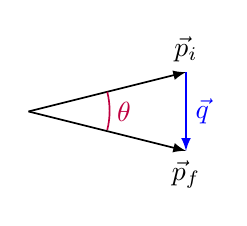
\begin{tikzpicture}
    \draw[semithick, -latex] (0,0) -- (2,0.5) node[above]{$\vec{p}_i$};
    \draw[semithick, -latex] (0,0) -- (2,-0.5) node[below]{$\vec{p}_f$};
    \draw[semithick, -latex, color=blue] (2,0.5) -- (2,-0.5);
    \draw[color=blue] (2,0) node[right]{$\vec{q}$};
    \draw[semithick, color=purple] (1,0.25) arc [radius=1, start angle=14.036, end angle=-14.036];
    \draw[color=purple] (1,0) node[right]{$\theta$};
  \end{tikzpicture}
  \caption{Impulso trasferito}
  \label{fig:impulso_trasferito}
\end{figure}

Con questa nuova definizione riprendiamo la sezione d'urto differenziale
dall'equzazione \ref{eq:sez_urto_diff_alpha} e sostuiamo l'equazione
\ref{eq:modulo_q} appena trovata:
\begin{align}
  \textbf{Sezione d'urto differenziale di Rutherford} &&
  \boxed{
    \frac{\md{\sigma}}{\md{\Omega}} = 4\mrb{zZ}^2 \alpha^2 \mrb{\hbar c}^2
    \frac{m^2}{q^4}
  }
  \label{eq:sezione_urto_differenziale_rutherford}
\end{align}

\begin{note}[]
  Nell'ipotesi di atomo \textit{non rinculante} c'è solo trasferimento di
  impulso, ma non c'è trasferimento di energia.
\end{note}

\subsection{Calcolo Quantistico della sezione d'urto}
Il calcolo quantistico della sezione d'urto dello scattering Rutherford può
essere effettuato utilizzando la \textit{Regola d'oro di Fermi}, definita come
segue:
\begin{align}
  \textbf{Regola d'Oro di Fermi} \qquad
  \boxed{
    \md{\omega_{if}} = \frac{2\pi}{\hbar} \, \abs{T_{if}^\prime}^2 \,
    \delta\mrb{E_i-E_f} \md{n_f}
  }
  \label{eq:regola_oro_fermi}
\end{align}
Dove $\ket{i}$ e $\ket{f}$ sono rispettivamente gli stati \textit{iniziale} e
\textit{finale} del processo e $\hat{\ham} = \hat{\ham}_{0} +
\hat{\ham}_{\text{int}}$ l'Hamiltoniana totale del sistema, definiamo le
seguenti grandezze:
\begin{itemize}
  \item $\md{\omega_{if}}$: probabilità di transizione per unità di tempo (le
    dimensioni fisiche saranno $\msb{\si{\per \s}}$);
  \item $E_i,E_f$: energie degli stati iniziale e finale;
  \item $T_{if}^\prime$: elemento di matrice;
    $\bra{f}\hat{\ham}_{\text{int}}\ket{i}$ dell'Hamiltoniana di interazione
  \item $\md{n_f}$: \# di stati finali accessibili per il sistema,
    ovvero\footnote{
      La grandezza $\rho\mrb{E_f}$ indica la densità di stati in funzione
      dell'energia e $\md{E}_{f}$ l'intervallo infinitesimo di energia
    } $\rho\mrb{E_f} \md{E_f}$;
  \item $\delta\mrb{E_f - E_i}$: delta di Dirac di \textbf{conservazione
    dell'energia}.
\end{itemize}

\paragraph{Definire stati iniziale e finale}
Supponiamo stati iniziale e finale \textit{autostati dell'impulso} (stati ad
impulso definito):
\begin{subequations}
  \begin{equation}
    \ket{i} = \ket{\vec{p}_i}
  \end{equation}
  \begin{equation}
    \ket{f} = \ket{\vec{p}_f}
  \end{equation}
\end{subequations}
Inoltre sappiamo gli autostati dell'impulso essere rappresentati nella base
degli \textit{autostati della posizione} da \textbf{onde piane}, quindi abbiamo
la forma seguente:
\begin{subequations}
  \begin{equation}
    \braket{\vec{x}\vert\vec{p}_i} = A \exp{\mcb{i \,
    \frac{\vec{p}_i\cdot\vec{x}}{\hbar}}}
  \end{equation}
  \begin{equation}
    \braket{\vec{x}\vert\vec{p}_f} = A \exp{\mcb{i
    \,\frac{\vec{p}_f\cdot\vec{x}}{\hbar}}}
  \end{equation}
  \label{eq:coordinate}
\end{subequations}
dove $A$ rappresenta la \textit{costante di normalizzazione delle onde piane}.

Presentiamo ora una procedura tipica in fisica delle particelle: fissiamo la
normalizzazione della funzione d'onda introducendo un \textit{volume di
normalizzazione}.

\paragraph{Volume di normalilzzazione}
La costante di normalizzazione può essere determinata in diversi modi. Uno di
questi è introdurre il \textbf{volume di normalizzazione} $V$, ovvero il volume
dello spazio tridimensionale all'interno del quale l'integrale del modulo
quadro della funzione d'onda sia uguale a 1. Facciamo questo per semplificare i
nostri calcoli, aspettandoci che il risultato finale sia indipendente dal
volume di normalizzazione utilizzato\footnote{
  Questo ci permette di determinare la normalizzazione degli stati, ma anche di
  calcolare il numero di stati finali accessibili dal sistema $\md{n_f}$,
  poiché questa è una grandezza che dipende da come normalizziamo i nostri
  stati
}. Quindi affinché gli stati
iniziale e finale siano normalizzati all'interno di tale volume di
normalizzazione, ovvero che:
\begin{equation}
  \braket{\vec{p}_{i,f} \vert \vec{p}_{i,f}} = 1 \rightarrow
  \mint{}{}{\vec{x}}{\abs{\braket{\vec{x} \vert \vec{p}_{i,f}}}^2} = 1
\end{equation}

Questo implica che il valore della costante $A$ nelle equazioni
\ref{eq:coordinate} sia $A = \frac{1}{\sqrt{V}}$, per cui:
\begin{subequations}
  \begin{equation}
    \braket{\vec{x}\vert\vec{p}_i} = \frac{1}{\sqrt{V}}\exp{\mcb{i \,
    \frac{\vec{p}_i\cdot\vec{x}}{\hbar}}}
  \end{equation}
  \begin{equation}
    \braket{\vec{x}\vert\vec{p}_f} = \frac{1}{\sqrt{V}}\exp{\mcb{i \,
    \frac{\vec{p}_f\cdot\vec{x}}{\hbar}}}
  \end{equation}
\end{subequations}

\begin{note}[]
  Dal punto di vista classico, una particella è identificata dalle $3$
  coordinate spaziali e dalle $3$ coordinate di impulso (\textit{spazio delle
  fasi classico}). Questo nel calcolo quantistico non vale, per cui diversi
  stati classici (nel limite del principio di indeterminazione) devono
  coincidere con un unico stato quantistico ($\Delta^3 x\, \Delta^3 p = h^3$).
  Quindi, avendo introdotto il \textit{volume di normalizzazione}, possiamo
  dire che $\Delta^3 x = V$, quindi: 
  \begin{equation}
    \Delta^3 p = \frac{h^3}{V}
  \end{equation}
  La \textit{densità dei possibili stati}:
  \begin{subequations}
    \begin{equation}
      \mdv{n_f}{p} = \frac{V}{h^3}
    \end{equation}
    quindi in termini di $\hbar$:
    \begin{equation}
      \mdv{n_f}{p} = \frac{V}{\mrb{2 \pi}^{3} \hbar^3}
    \end{equation} 
  \end{subequations}
\end{note}

A questo punto possiamo andare a calcolare l'elemento di matrice
$T_{if}^\prime$, ricordando che $\hat{\ham}_{\text{int}}$ è il
\textit{potenziale coulombiano} generato dal nucleo scatterante:
\begin{equation}
  T_{if}^\prime = \bra{f}\ham_{\text{int}}\ket{i} = \int \mathrm{d}^3\vec{x}
  \int \, \mathrm{d}^3\vec{y} \braket{f\vert\vec{x}\,}
  \bra{\vec{x}\,}\ham_{\text{int}} \ket{\vec{y}\,} \, \braket{\vec{y}\,\vert i}
  \label{eq:elemento_matrice_hamilt_interazione}
\end{equation}
poiché gli integrali sui proiettori $\ket{\vec{x}\,}\bra{\vec{x}\,}$ e
$\ket{\vec{y}\,}\bra{\vec{y}\,}$ sono proprio l'identità. Poiché possiamo
scrivere l'Hamiltoniana di interazione come (\textit{interazione
coulombiana}\footnote{
  I potenziali di interazione che hanno andamento $\frac{1}{r}$ sono detti
  \textbf{potenziali a lungo raggio}
} dipendente solo dalla posizione),
scegliendo un sistema di riferimento in cui la particella che produce lo
scattering è posta nell'origine:
\begin{equation}
  \hat{\ham}_{\text{int}} = \frac{zZe^2}{4\pi\epsilon_0} \,
  \frac{1}{\abs{\vec{x}}\,}
  \label{eq:ham_int_puntiforme}
\end{equation}
dove chiaramente $z$ è la carica della particella scatterata e $Z$ la carica
del nucleo che produce l'effetto di scattering.
Quindi il termine $\bra{\vec{x}}\ham_{\text{int}}\ket{\vec{y}\,}$ farà
comparire una $\delta$ del tipo:
\begin{equation}
  \braket{\vec{x}\, \vert \hat{\ham} _{\text{int}} \vert \vec{y}\,} = 
  \frac{zZe^2}{4\pi\epsilon_0} \, \frac{1}{\abs{\vec{x}}} \, \delta^{(3)}
  \mrb{\vec{x} - \vec{y}\,}
\end{equation}
La delta rimuoverà uno dei due integrali\footnote{Vedi proprietà della Delta di
Dirac}, quindi continuiamo il calcolo dell'elemento di matrice riprendendo
dall'equazione \ref{eq:elemento_matrice_hamilt_interazione}:
\begin{equation}
  \begin{split}
    T_{if}^\prime & = \frac{1}{V} \int \mathrm{d}^3\vec{x} \, \exp{\mcb{-i \,
    \frac{\vec{p}_f\cdot\vec{x}}{\hbar}}} \,
    \hat{\ham}_{\text{int}}\mrb{\vec{x}\,} \, \exp{\mcb{i \,
    \frac{\vec{p}_i\cdot\vec{x}}{\hbar}}} \\
    & = \frac{1}{V} \int \mathrm{d}^3\vec{x} \,  \exp\mcb{-i \,
    \frac{\mrb{\vec{p}_f-\vec{p}_i}\cdot\vec{x}}{\hbar}} \,
    \hat{\ham}_{\text{int}}\mrb{\vec{x}\,} \\
    & = \frac{1}{V} \int \mathrm{d}^3\vec{x} \,  \exp\mcb{-i \,
    \frac{\mrb{\vec{p}_f-\vec{p}_i}\cdot\vec{x}}{\hbar}} \,
    \frac{zZe^2}{4\pi\epsilon_0} \, \frac{1}{\abs{\vec{x}}}
  \end{split}
\end{equation}
ed esprimendo in termini della quantità vettoriale \textit{impulso trasferito}
definita dall'equazione \ref{eq:impulso_trasferito}:
\begin{equation}
  T_{if}^\prime = \frac{1}{V} \int \mathrm{d}^3\vec{x} \, \exp\mcb{-i \,
  \frac{\vec{q}\cdot\vec{x}}{\hbar}} \, \frac{zZe^2}{4\pi\epsilon_0} \,
  \frac{1}{\abs{\vec{x}}}
  \label{eq:elemento_matrice_T_puntiforme}
\end{equation}
\textbf{Nota:} possiamo osservare che questa quantità, a meno della costante di
normalizzazione, è proporzionale alla \textit{\textbf{trasformata di Fourier}}
del potenziale di interazione con parametro della trasformazione definito
dall'impulso trasferito.
Questo ci dice che tanto maggiore è l'impulso trasferito, tanto più piccole
saranno le strutture che si possono osservare dei potenziali che mediano una
certa interazione (questo vale in generale, non solo per scattering
Rutherford).

Per calcolare l'integrale dato dall'equazione
\ref{eq:elemento_matrice_T_puntiforme} scegliamo un sistema di riferimento che
vede il vettore $\vec{q}$ diretto lungo l'asse $\hat{z}$ e il nucleo
scatterante posto nell'origine, come in figura:

\begin{figure}[ht]
  \centering
  \tdplotsetmaincoords{60}{110}
  \begin{tikzpicture}[scale=3,tdplot_main_coords]

    % variables
    \def\rvec{.8}
    \def\thetavec{30}
    \def\phivec{60}

    % axes & vector
    \coordinate (O) at (0,0,0);
    \draw[thick,-latex] (0,0,0) -- (1,0,0) node[anchor=north east]{$x$};
    \draw[thick,-latex] (0,0,0) -- (0,1,0) node[anchor=north west]{$y$};
    \draw[thick,-latex] (0,0,0) -- (0,0,1) node[anchor=south]{$z$};
    \draw[thick,-latex, color=blue] (0,0,0) -- (0,0,0.4) node[left]{$\vec{q}$};
    \tdplotsetcoord{P}{\rvec}{\thetavec}{\phivec}
    \draw[-latex,color=red, semithick] (O) -- (P) node[above right] {$\vec{r}$};

    % arcs
    \draw[dashed, color=red] (O) -- (Pxy);
    \draw[dashed, color=red] (P) -- (Pxy);
    \tdplotdrawarc{(O)}{0.2}{0}{\phivec}
    {anchor=north}{$\varphi$}
    \tdplotsetthetaplanecoords{\phivec}
    \tdplotdrawarc[tdplot_rotated_coords]{(0,0,0)}{0.5}{0}{\thetavec}
    {anchor=south west}{$\theta$}

  \end{tikzpicture}
  \caption{Scelta del sistema di riferimento}
  \label{fig:sistema_riferimento}
\end{figure}

Per cui l'equazione \ref{eq:elemento_matrice_T_puntiforme} diventa (dove
abbiamo utilizzato la notazione $r = \abs{\vec{x}}$ e $q = \abs{\vec{q}\,}$):
\begin{subequations}
  \begin{equation}
    \begin{split}
      T_{if}^\prime 
      & = \frac{1}{V} \int_0^{2\pi} \! \mathrm{d}\varphi \int_{-1}^{1} \!
      \mathrm{d}\cos\theta \int_0^\infty \! \mathrm{d}r \,r^{\cancel2} \,
      \exp\mcb{i \, \frac{qr \cos\theta}{\hbar}} \frac{zZe^2}{4\pi\epsilon_0}
      \, \frac{1}{\cancel r}
      \\
      & = \frac{2 \pi}{V} \, \frac{zZe^2}{4\pi\varepsilon_0} \int_{-1}^{1} \!
      \mathrm{d}\cos\theta \int_0^\infty \! \mathrm{d}r \,r \exp\mcb{i \,
      \frac{qr \cos\theta}{\hbar}}
    \end{split}
    \label{eq:calcolo_elemento_matrice_T}
  \end{equation}
  per semplificare la notazione introduciamo la variabile $k = \frac {q}{r}$,
  per cui integrando prima in $\cos\theta$:
  \begin{equation}
    \begin{split}
      T_{if}^\prime 
      & = \frac{2 \pi}{V} \, \frac{zZe^2}{4\pi\varepsilon_0} \int_0^\infty \!
      \mathrm{d}r \, \cancel r \frac{1}{ik \cancel r} \mcb{\exp\msb{ikr} -
      \exp\msb{-ikr}} \\
      & = \frac{2 \pi}{V} \, \frac{zZe^2}{4\pi\varepsilon_0} \,
      \frac{1}{\mrb{ik}^2} \mcb{\exp\msb{ikr}_0^\infty +
      \exp\msb{-ikr}_0^\infty}
    \end{split}
  \end{equation}
\end{subequations}
Ora, poiché $\exp\msb{ikr}$ ed $\exp\msb{-ikr}$ sono \textit{soluzioni
oscillanti \textbf{non} dumpate}, l'integrale non converge. Abbiamo il problema
che non possiamo valutare esplicitamente l'integrale. Questo è legato al fatto
che il modello considerato è poco realistico, nel senso che il potenziale di
interazione considerato ha lo stesso comportamento in tutto lo spazio\footnote{
  Non viene considerata, ad esempio, l'azione schermante degli elettroni
  atomici degli atomi scatteranti. Infatti, a distanze minori della dimensioni
  caratteristiche dell'atomo l'interazione si sente; a distanze maggiori,
  invece, gli elettroni atomici schermano la carica del nucleo e l'interazione
  è dumpata
}. Nella realtà accade che ci sarà sempre una \textit{lunghezza di taglio}
oltre la quale il potenziale risulta schermato.

\paragraph{Taglio al potenziale di interazione} Ripetiamo ora il calcolo
dell'elemento introducendo un \textit{taglio (dump) esponenziale} al potenziale
di interazione coulombiano, che è un potenziale a corto raggio, per cui
riscriviamo l'Hamiltoniana di interazione come:
\begin{equation}
  \hat{\ham}_{\text{int}} = \frac{zZe^2}{4 \pi \varepsilon_0} \, \frac{1}{r}
  \exp\msb{-\mu r}
\end{equation}
dove $\mu$ può essere espresso in termini della lunghezza caratteristica $r_t$
chiamata \textbf{raggio di taglio}:
\begin{equation}
  \mu = \frac{1}{r_t}
\end{equation}
Si utilizza il taglio esponenziale poiché:
\begin{itemize}
  \item se $r \ll r_t$ l'Hamiltoniana di interazione descrive correttamente gli
    effetti coulombiani
  \item se $r \gg r_t$ il termine esponenziale sopprime l'interazione
    coulombiana
\end{itemize}
Torniamo al calcolo dell'integrale che descrive l'elemento di matrice
$T_{if}^\prime$, lasciato all'equazione \ref{eq:calcolo_elemento_matrice_T}
inserendo il termine aggiuntivo di taglio:
\begin{subequations}
  \begin{equation}
    \begin{split}
      T_{if}^\prime 
      & = \frac{2\pi}{V} \, \frac{zZe^2}{4\pi\varepsilon_0} \int_{-1}^{1} \!
      \mathrm{d}\cos\theta \int_0^\infty \! \mathrm{d}r \, r e^{-\mu r}
      e^{ikr \cos\theta} \\
      & = \frac{2\pi}{V} \, \frac{zZe^2}{4\pi\varepsilon_0} \int_0^\infty \!
      \mathrm{d}r \, \frac{\cancel r}{ik \cancel r} e^{-\mu r} \,
      \mcb{e^{ikr} - e^{-ikr}} \\
      & = \frac{2\pi}{V} \, \frac{zZe^2}{4\pi\varepsilon_0} \int_0^\infty \!
      \mathrm{d}r \, \frac{1}{ik} \mcb{e^{-\mrb{\mu - ik}r} -
      e^{-\mrb{\mu + ik}r}} \\
      & = \frac{2\pi}{V} \, \frac{zZe^2}{4\pi\varepsilon_0} \, \frac{1}{ik}
      \mcb{\frac{1}{-\mrb{\mu - ik}} e^{-\mrb{\mu-ik}r}\Big\rvert_0^\infty -
      \frac{1}{-\mrb{\mu + ik}} e^{-\mrb{\mu+ik}r}\Big\rvert_0^\infty}
    \end{split}
  \end{equation}
  e poiché gli esponenziali, dumpati dall'introduzione di $\mu$, sono nulli se
  valutati all'infinito, l'espressione si riduce a:
  \begin{equation}
    \begin{split}
      T_{if}^\prime 
      & = - \frac{2\pi}{V} \, \frac{zZe^2}{4\pi\varepsilon_0} \, \frac{1}{ik}
      \mcb{\frac{1}{-\mrb{\mu - ik}} - \frac{1}{-\mrb{\mu + ik}}} \\
      & = \frac{2\pi}{V} \, \frac{zZe^2}{4\pi\varepsilon_0} \, \frac{1}{ik}
      \mcb{\frac{\cancel\mu + ik - \cancel\mu + ik}{\mrb{\mu - ik}
      \mrb{\mu + ik}}} \\ 
      & = \frac{2\pi}{V} \, \frac{zZe^2}{4\pi\varepsilon_0} \, \frac{2}{\mu^2 +
      k^2}
    \end{split}
  \end{equation}
\end{subequations}
Quindi con il taglio esponenziale, e il parametro $\mu$, siamo in grado di
calcolare l'elemento di matrice:
\begin{equation}
  \textbf{Potenziale di Yukawa}\text{ ($r_t$ finita)}\qquad
  \boxed{
    T_{if}^\prime = \frac{4\pi}{V} \, \frac{zZe^2}{4\pi\varepsilon_0} \,
    \frac{1}{\mu^2 + k^2}
  }
\end{equation}
Nel caso \textit{coulombiano} mandiamo all'infinito la lunghezza di taglio
$r_t$ e otteniamo:
\begin{equation}
  T _{if} \mprime \xrightarrow{r_t \to \infty\ \Rightarrow\ \mu \to 0}
  \frac{4 \pi}{V} \frac{zZe^2}{4 \pi \eps_0} \frac{1}{k^2}
\end{equation}

Riprendendo la \textit{Regola d'oro di Fermi} (equazione
\ref{eq:regola_oro_fermi}), l'espressione che si ottiene quando
\textbf{rimuoviamo la lunghezza di taglio} $r_t$, ovvero quando $\mu \to 0$: 
\begin{equation}
  \begin{split}
    \md{\omega_{if}} 
    & = \frac{2\pi}{\hbar} \, \abs{T_{if}^\prime}^2 \, \delta\mrb{E_i - E_f}
    \, \md{n_f} \\
    & = \frac{2\pi}{\hbar} \, \mrb{\frac{4\pi}{V}}^2
    \mrb{\frac{zZe^2}{4\pi\varepsilon_0}}^2 \frac{1}{k^4} \,
    \delta\mrb{E_i - E_f} \, \md{n_f}
  \end{split}
  \label{eq:fermi_quasi_esplicita}
\end{equation}
Manipolando i termini per cercare un'espressione più compatta della formula,
con $\alpha$ la \textit{costante di struttura fine}:
\begin{equation}
  \frac{zZe^2}{4\pi\varepsilon_0} = \frac{zZe^2}{4\pi\varepsilon_0} \,
  \frac{\hbar c}{\hbar c} = zZ \alpha \hbar c
\end{equation}
in più, ricordando che $k = \nicefrac{q}{\hbar}$, ritroviamo un risultato già
ottenuto nel caso classico (equazione
\ref{eq:sezione_urto_differenziale_rutherford}) nella dipendenza da potenziale
coulombiano: in questo caso osserviamo che il tasso di transizione
$\md{\omega_{if}} \sim q^{-4}$.  
Riscriviamo la \ref{eq:fermi_quasi_esplicita}, ricordando che $k =
\frac{q}{\hbar}$:
\begin{equation}
  \md{\omega_{if}} = \frac{2\pi}{\hbar} \mrb{\frac{4\pi}{V}}^2 \mrb{zZ}^2
  \alpha^2 \mrb{\hbar c}^2 \frac{\hbar^4}{q^4} \, \delta\mrb{E_i - E_f}
  \md{n_f}
\end{equation}
\paragraph{Numero di stati finali accessibili dal sistema}
Ci rimane valutare il numero di stati finali accessibili dal sistema, ovvero la
\textit{conta degli stati} $\md{n_f}$.
Questo si può fare \textbf{imponendo le condizioni al bordo} oppure sfruttando
il \textbf{principio di corrispondenza}. Definiamo il \textbf{volume dello
spazio delle fasi classico occupato da uno stato quantistico}: uno stato
quantistico, occupa nello spazio delle fasi classico, dato il \textit{principio
di indeterminazione di Heisenberg}, un volume dato da:
\begin{equation}
  \boxed{\Delta^3p \, \Delta^3x = h^3}
\end{equation}
dove $\Delta^3x = V$ è proprio il \textit{volume di normalizzazione}, per cui
fissando lo spazio fisico in questo modo:
\begin{equation}
  \Delta^3p = \frac{h^3}{V}
\end{equation}
Per cui:
\begin{equation}
  \md{n_f} = \frac{\mathrm{d}^3p}{h}V
\end{equation}
Quindi possiamo dire che il numero degli stati finali accessibili dal sistema
ha una densità costante\footnote{
  La densità degli stati finali è \textit{uniforme} in $p$, poiché non c'è
  motivo che un impulso sia preferito rispetto ad un altro (\textit{isotropia})
} data da:
\begin{equation}
  \boxed{
    \frac{\md{n_f}}{\mathrm{d}^3p} = \frac{V}{h^3} = \frac{V}{\hbar^3
    \mrb{2\pi}^3}
  }
\end{equation}

\paragraph{Tasso di transizione}
In conclusione, mettendo insieme tutti i risultati ricavati fino ad ora,
possiamo dire che la \textit{probabilità di transizione per unità di tempo} per
il processo di \textit{scattering Rutherford} è data da:
\begin{equation}
  \md{\omega_{if}} = \frac{2\pi}{\cancel\hbar} \mrb{\frac{4\pi}{V}}^2 \alpha^2
  \mrb{\hbar c}^2 \frac{\cancel{\hbar^4}}{q^4} \mrb{zZ}^2
  \delta\mrb{E_i - E_f} \frac{V}{\cancel{\hbar^3} \mrb{2\pi}^3} \,
  \mathrm{d}^3p_f
  \label{eq:prob_transizione_unita_tempo}
\end{equation}
osserviamo che la quantità $\md{d}\omega_{if}$, ovvero la probabilità di
transizione per unità di tempo, conserva la dipendenza dal volume di
normalizzazione $V$. Questa quantità, però, non è l'osservabile fisico. Per
questo motivo andiamo a calcolare la sezione d'urto.

\paragraph{Sezione d'urto quantistica per Scattering Rutherford}
La sezione d'urto di questo processo è legata alla probabilità di transizione
per unità di tempo $d\omega_{if}$. La sezione d'urto ci dice quanto è probabile
che un processo di interazione fra ``\textit{proiettile}'' e
``\textit{bersaglio}'' avvenga.

In particolare, in questo caso abbiamo che il numero di eventi per unità di
tempo e per unità di tempo e unità di impulso dello stato finale:
\begin{equation}
  \frac{\md{N_\text{eventi}}}{\md{t} \, \mathrm{d}^3p_f} =
  \frac{\md{\sigma}}{\mathrm{d}^3p_f} \,
  \phi_p \,  N_t
\end{equation}
dove le quantità sono:
\begin{itemize}
  \item $\phi_p$ il \textit{flusso delle particelle (proiettili) incidenti};
  \item $N_t$ il \textit{numero di bersagli} illuminati dal fascio
    (\textit{numero di target});
  \item $\frac{\md{\sigma}}{\mathrm{d}^3p_f}$ la \textit{sezione d'urto
    differenziale} del processo definita in funzione dell'impulso della
    particella nello stato finale.
\end{itemize}
Ricordiamo che nel nostro caso particolare si considera un singolo processo
(una particella su singolo bersaglio) all'interno di un volume di
normalizzazione, per cui, all'interno di quest'ultimo possiamo dire che:
\begin{equation}
  \begin{dcases}
    N_t = 1 \\
    \phi_p = nv = \frac{1}{V} v \\
    \frac{\md{N_\text{eventi}}}{\md{t} \, \mathrm{d}^3p_f} =
    \frac{\md{\omega_{if}}}{\mathrm{d}^3p_f}
  \end{dcases}
\end{equation}
Dove per il flusso $\phi_p$: $v$ indica la \textit{velocità}
della particella $z$ incidente e $n$ indica la ``\textit{number density}'' di
particelle $z$ che collidono con il nucleo scatteratore e nel nostro caso
risulta essere $\nicefrac{v}{V}$ perché consideriamo una particella all'interno
del volume di normalizzazione.

Quindi possiamo scrivere che la sezione d'urto vale:
\begin{equation}
  \frac{\md{\sigma}}{\mathrm{d}^3p_f} = \frac{\md{N_\text{eventi}}}{\md{t} \,
  \mathrm{d}^3p_f} \, \frac{1}{\phi_\text{proiettili} N_t} =
  \frac{\md{\omega_{if}}}{\mathrm{d}^3p_f} \, \frac{V}{v}
\end{equation}
e sfruttando l'equazione \ref{eq:prob_transizione_unita_tempo}:
\begin{equation}
  \frac{\md{\sigma}}{\mathrm{d}^3p_f} = \msb{2\pi \mrb{\frac{4\pi}{\cancel
  V}}^2 \alpha^2 \mrb{\hbar c}^2 \frac{1}{q^4} \mrb{zZ}^2 \delta\mrb{E_i -
  E_f} \frac{\cancel V}{\mrb{2\pi}^3}} \frac{\cancel V}{v}
\end{equation}
quindi osserviamo che ora la sezione d'urto differenziale risulta del tutto
indipendente dal volume di normalizzazione $V$ e possiamo rielaborare e
semplificare ulteriormente ottenendo:
\begin{equation}
  \frac{\md{\sigma}}{\mathrm{d}^3p_f} = 4 \mrb{\hbar c}^2 \alpha^2 \mrb{zZ}^2
  \delta\mrb{E_i - E_f} \frac{1}{v} \, \frac{1}{q^4}
\end{equation}
In più, nel limite in cui il nucleo scatterante non rinculi, si avrebbe che
l'impulso finale $p_i$ coincide con l'impulso finale $p_f$ e si può descrivere
tutta la dinamica in termini dell'angolo solido $\Omega$, poiché potendo
scrivere:
\begin{equation}
  \mathrm{d}^3p_f = p_f^2 \md{p_f} \, \md{\Omega }
\end{equation}
dove abbiamo integrato su tutto il range di impulsi, per ottenere
un'espressione della sezione d'urto differenziale solo rispetto all'angolo
solido. Segue che:
\begin{subequations}
  \begin{equation}
    \frac{\md{\sigma}}{\md{\Omega}} = \int_0^\infty \!
    \frac{\md{\sigma}}{\mathrm{d}^3p_f} \, p_f^2 \, \md{p_f} = \int_0^\infty \!
    4 \mrb{\hbar c}^2 \alpha^2 \mrb{zZ}^2 \delta\mrb{E_i - E_f} \frac{1}{v} \,
    \frac{1}{q^4} \, p_f^2 \, \md{p_f}
  \end{equation}
  Ora se stiamo parlando di una \textit{particella incidente non
  relativistica}, possiamo riscrivere le quantità $E_f$ e $v$ in termini
  dell'impulso $p_f$, dove $m$ è la massa della particella:
  \begin{equation}
    \frac{\md{\sigma}}{\md{\Omega}} = \int_0^\infty \! 4 \mrb{\hbar c}^2
    \alpha^2 \mrb{zZ}^2 \delta\mrb{E_i - \frac{p_f^2}{2m}} \frac{m}{p_f} \,
    \frac{1}{q^4} \, p_f^2 \, \md{p_f}
  \end{equation}
  Poiché la delta di Dirac di conservazione dell'energia è espressa in termini
  di $p^2_f$, cambiamo variabile di integrazione con quest'ultima come segue:
  \begin{equation}
    \frac{\md{\sigma}}{\md{\Omega}} = \int_0^\infty \frac{\cancel 2
    m^2}{\bcancel{2 p_f}} \, \frac{\cancel{p_f^2}}{\cancel{p_f}} 4 \mrb{\hbar
    c}^2 \alpha^2 \mrb{zZ}^2 \delta\mrb{E_i - \frac{p_f^2}{2m}} \frac{1}{q^4}
    \, \md{\mrb{\frac{p_f^2}{2m}}}
  \end{equation}
  La Delta seleziona il modulo dell'impulso finale $p_f$ in modo che sia uguale
  all'impulso iniziale $p_i$ affinché l'energia rimanga conservata, per cui
  rimuove l'integrale e si ottiene il risultato finale:
  \begin{align}
    \textbf{Sezione d'urto differenziale di Rutherford} &&
    \boxed{
      \frac{\md{\sigma}}{\md{\Omega}} = 4 \mrb{\hbar c}^2 \alpha^2 \mrb{zZ}^2
      \frac{m^2}{q^4}
    }
  \end{align}
\end{subequations}
Possiamo osservare in più che, poiché la Delta di conservazione dell'energia
fissa il modulo dell'impulso finale della particella scatterata, $p_f$, la
quantità \textit{impulso trasferito} $q$ dipenderà esclusivamente dall'angolo
di deflessione:
\begin{equation}
  q = 2 p \sin \frac{\theta}{2}
\end{equation}
dove $p = \abs{\vec{p}_i} = \abs{\vec{p}_f}$.
\begin{note}[]
  Il risultato ottenuto dal calcolo quantistico corrisponde esattamente al
  risultato trovato dal calcolo classico!
\end{note}

%LTeX: language=it
% TODO: rivedere bene questa lezione sfruttando la registrazione del 28 aprile 2022
\chapter{Lezione 2020-05-07}
\section{Scattering Rutherford (reprise)}
Fino ad ora abbiamo lavorato in approssimazione di \textit{nucleo puntiforme}.
Questa approssimazione non è più adeguata se vogliamo andare a studiare gli
effetti della dimensione finita del nucleo o studiare la dimensione del nucleo
stesso. Quindi il quesito che ci poniamo è: \textit{come varia l'espressione
	della sezione d'urto differenziale di Rutherford se rimuoviamo
	l'approssimazione di nucleo puntiforme}?

\subsection{Sezione d'urto per nucleo \textit{non} puntiforme}
Consideriamo il nucleo atomico come una distribuzione estesa di carica per
cui\footnote{
	La notazione utilizzata prevede che $\vec{r}$ sia il vettore e $r$ il suo
	modulo
}:
\begin{itemize}
	\item $\rho(\vec{r}\,)$: \textit{densità di carica} $\longrightarrow \int
		      \rho(\vec{r}\,) \, \mathrm{d}^3r = Ze$
	\item $\rho_N \mrb{\vec{r}\,} = \dfrac{\rho\mrb{\vec{r}\,}}{Ze}$:
	      \textit{densità di carica normalizzata} $\longrightarrow \int
		      \rho_N\mrb{\vec{r}\,} \, \mathrm{d}^3r = 1$
\end{itemize}
Questa modifica alle ipotesi di lavoro si ripercuote nell'espressione che
descrive l'Hamiltoniana di interazione $\ham_\text{int}$.

\paragraph{Elemento di matrice per distribuzione estesa di carica}
In generale, l'elemento di matrice $T_{if}$ si calcola come:
\begin{equation}
	T_{if} = \braket{f \vert \ham_\text{int} \vert i}
\end{equation}
che abbiamo già visto nel caso puntiforme nelle equazioni
\ref{eq:ham_int_puntiforme} e \ref{eq:elemento_matrice_T_puntiforme}.

Nel caso \textit{non} puntiforme avremo quindi che l'Hamiltoniana di
interazione assume la seguente forma:
\begin{equation}
	\ham_\text{int} \mrb{\vec{r}\,} = \frac{ze}{4\pi \varepsilon_0} \int
	\frac{\rho\mrb{\vec{r}\mprime}}{\abs{\vec{r} - \vec{r}\,\mprime}} \,
	\mathrm{d}^3r\mprime
	= \frac{zZe^2}{4\pi \varepsilon_0} \int
	\frac{\rho_N\mrb{\vec{r}\mprime}}{\abs{\vec{r} - \vec{r}\,\mprime}} \,
	\mathrm{d}^3r\mprime
	\label{eq:ham_int_estesa}
\end{equation}
dove l'integrale è valutato in \textit{tutto lo spazio} e $\abs{\vec{r} -
		\vec{r}\,\mprime}$ indica la distanza fra il punto $\vec{r}$ in cui voliamo
valutare l'interazione e il punto $\vec{r}\,\mprime$ dell'elemento infinitesimo
di carica della distribuzione estesa che la genera. Quindi abbiamo
l'espressione esplicita del \textit{potenziale elettrostatico generato da una
	distribuzione arbitraria di carica}.

Quindi quando consideriamo la distribuzione estesa, otteniamo l'elemento di
matrice $T_{if}$ effettuando la trasformata di Fourier di
\ref{eq:ham_int_estesa}. Per cui:
\begin{subequations}
	\begin{equation}
		T_{if} = \frac{1}{V} \, \frac{zZe^2}{4\pi \varepsilon_0} \int \mathrm{d}^3r
		\! \int \mathrm{d}^3r\mprime \,
		\frac{\rho_N(\vec{r}\,\mprime)}{\abs{\vec{r} - \vec{r}\,\mprime}}
		\exp\mcb{i \, \frac{\mrb{\vec{p}_f - \vec{p}_i} \cdot \vec{r}}{\hbar}}
	\end{equation}
	Ma espressa in questo modo è di difficile risoluzione, quindi moltiplichiamo
	e dividiamo per \\ $\exp\mcb{-i \, \frac{\mrb{\vec{p}_f - \vec{p}_i} \cdot
				\vec{r}\,\mprime}{\hbar}}$ e otteniamo:
	\begin{equation}
		T_{if} = \frac{1}{V} \, \frac{zZe^2}{4\pi \varepsilon_0} \int \mathrm{d}^3r
		\! \int \mathrm{d}^3r\mprime \,
		\frac{\rho_N(\vec{r}\,\mprime)}{\abs{\vec{r} - \vec{r}\,\mprime}}
		\exp\mcb{i \, \frac{\mrb{\vec{p}_f - \vec{p}_i} \cdot \mrb{\vec{r} -
					\vec{r}\,\mprime}}{\hbar}} \exp\mcb{i \, \frac{\mrb{\vec{p}_f - \vec{p}_i}
				\cdot \vec{r}\,\mprime}{\hbar}}
	\end{equation}
	Osserviamo che ora la possiamo separare gli integrali nelle variabili
	$\vec{r}\,\mprime$ e $\vec{r}\,\mdprime = \vec{r} - \vec{r}\,\mprime$, come
	prodotto di due termini calcolabili in maniera indipendente, come segue:
	\begin{equation}
		T_{if} = \frac{1}{V} \, \frac{zZe^2}{4\pi \varepsilon_0} \int
		\mathrm{d}^3r\mdprime \, \frac{1}{r\mdprime} \exp\mcb{i \,
			\frac{\mrb{\vec{p}_f - \vec{p}_i} \cdot \vec{r}\,\mdprime}{\hbar}} \int
		d^3r\mprime \, \rho_N\mrb{\vec{r}\,\mprime} \exp\mcb{i \,
			\frac{\mrb{\vec{p}_f - \vec{p}_i} \cdot \vec{r}\,\mprime}{\hbar}}
	\end{equation}
\end{subequations}
In più il \textit{primo dei due termini moltiplicativi}, inclusi i prefattori,
costituiscono esattamente la trasformata di Fourier del potenziale puntiforme,
per cui rappresenta l'elemento di matrice del potenziale puntiforme già
calcolata in precedenza\footnote{
	Siamo passati ad utilizzare la quantità \textit{impulso trasferito} $\vec{q}$
}.
\begin{equation}
	\mrb{T_{if}}_\text{punt} = \frac{1}{V} \, \frac{zZe^2}{4\pi \varepsilon_0}
	\int d^3r\mdprime \, \frac{1}{r\mdprime} \exp\mcb{i \, \frac{\vec{q} \cdot
			\vec{r}\,\mdprime}{\hbar}}
\end{equation}
Il \textit{secondo termine moltiplicativo} rappresenta, invece, la
trasformazione di Fourier della distribuzione normalizzata di carica,
$\rho_N\mrb{\vec{r}\,\mprime}$, con parametro di trasformazione (quindi con
vettore d'onda) $\frac{\vec{q}}{\hbar}$. Questo oggetto è una funzione
complessa di $\vec{q}$ ed e assume il nome di \textit{fattore di forma
	associato alla distribuzione di carica} considerata:
\begin{align}
	\textbf{Fattore di Forma}
	\qquad
	\boxed{
		F\mrb{\vec{q}\,} = \int d^3r\mprime \, \rho_N\mrb{\vec{r}\,\mprime}
		\exp\mcb{i \, \frac{\vec{q} \cdot \vec{r}\,\mprime}{\hbar}}
	}
\end{align}
e rappresenta la modifica che si apporta all'elemento di matrice del caso
puntiforme per passare alla distribuzione estesa di carica.\\
\begin{note}[]
	Il \textit{fattore di forma} non è altro che la \textit{trasformata di
		Fourier della distribuzione di carica} del nucleo scatteratore.
\end{note}
\begin{note}[]
	Qualora il sistema che si sta considerando fosse dotato di \textit{simmetria
		sferica} la dipendenza di $F$ da $\vec{q}$ riguarderebbe solo il modulo,
	ovvero $F = F\mrb{\vec{q}\,}$.
\end{note}

Alla luce di queste considerazioni possiamo scrivere l'elemento di matrice come segue:
\begin{equation}
	\boxed{
		T_{if} = \mrb{T_{if}}_\text{punt} F\mrb{\vec{q}\,}
	}
\end{equation}

\paragraph{Sezione d'urto differenziale di Rutherford per distribuzione estesa
	di carica}
Tenendo conto di questa nuova espressione dell'elemento di matrice di interazione, omettendo tutti i passaggi che formalmente prevedono che si sostituisca quest'ultima nell'espressione della regola d'oro di Fermi (equazione \ref{eq:regola_oro_fermi}) e che si proceda analogamente al caso puntiforme, scriviamo la \textit{sezione d'urto differenziale per scattering Rutherford in ipotesi di nucleo come distribuzione estesa di carica}:
\begin{align}
	\textbf{Sezione d'urto differenziale per distribuzione estesa} &  &
	\boxed{
		\frac{d\sigma}{d\Omega} = \mrb{\frac{d\sigma}{d\Omega}}_\text{punt}
		\abs{F\mrb{\vec{q}\,}}^2
	}
\end{align}

\begin{note}[]
	Attenzione, perché questo approccio non determina univocamente
	la funzione $F\mrb{\vec{q}\,}$, ma ne determina solo il modulo; non abbiamo
	alcuna informazione sulla fase. Quindi, ad esempio, non possiamo utilizzare
	questo approccio per la ricostruzione del \textit{fattore di forma} da dati
	sperimentali antitrasformando, perché di nuovo, abbiamo che i dati
	eventualmente ottenuti sarebbero legati solo al modulo di $F$.
\end{note}

\subsection{Deviazione dal comportamento puntiforme}
Studiando le deviazioni del \textit{fattore di forma} dall'unità si possono
valutare le dimensioni dei nuclei.
Della definizione di \textit{fattore di forma},  in ipotesi di simmetria
sferica, distinguiamo i seguenti casi:
\begin{itemize}
	\item $\mrb{\frac{q}{\hbar}} R_N \ll 1$ nelle regioni di spazio in cui la
	      distribuzione normalizzata di carica è sensibilmente diversa da 0 si ha
	      che:
	      \begin{equation}
		      F\mrb{q \simeq 0} = 1
	      \end{equation}
	      per cui gli urti che avvengono con un impulso trasferito piccolo si possono
	      considerare urti fra particelle puntiformi. Quindi
	      \textit{non possiamo utilizzare urti con} $q \simeq 0$ \textit{per studiare
		      le dimensioni del nucleo}.
	\item $\mrb{\frac{q}{\hbar}} R_N \gtrsim 1$ nelle regioni di spazio in cui la
	      distribuzione normalizzata di carica è sensibilmente diversa da 0 si ha
	      che:
	      \begin{equation}
		      F\mrb{q} \neq 1
	      \end{equation}
\end{itemize}
Come già visto nell'equazione \ref{eq:modulo_q} che riportiamo nuovamente di
seguito (in riferimento alla figura \ref{fig:impulso_trasferito}), se $p =
	\abs{\vec{p}_i} = \abs{\vec{p}_f}$:
\begin{equation}
	\abs{\vec{q}\,} = 2p \, \sin\frac{\theta}{2}
\end{equation}
avremo che ad impulso fissato l'impulso trasferito dipenderà dall'angolo
$\theta$. Quindi al variare di tale angolo si registreranno diversi valori di
$q$; per cui avremo che, tramite il fattore di forma, l'angolo $\theta$ modula
la sezione d'urto.

Ora, sapendo che i nuclei hanno dimensioni caratteristiche dell'ordine del
fermi, possiamo chiederci quale sia la condizione sull'impulso trasferito $q$
che causa le deviazioni che ci permettano di studiare le dimensioni del nucleo:
\begin{equation}
	q \gtrsim \frac{\hbar c}{R_N c} \implies qc \gtrsim \frac{\hbar c}{R_N}
	\simeq \frac{\qty{200}{\MeV \femto\meter}}{R_N \: \msb{\si{\femto\meter}}}
\end{equation}
quindi l'impulso trasferito per sondare strutture (nel nostro caso nulcei)
dalle dimensioni dell'ordine di grandezza del \textit{fermi} deve essere
dell'ordine di centinaia di \si{\MeV \per c}.

\section{Modelli per la distribuzione di carica nei nuclei}
% TODO: da qui ci sono state delle differenze nella notazione
\subsection{Sfera uniformemente carica}
Definiamo una distribuzione di carica la cui densità (normalizzata) dipenda
solo dalla distanza dal baricentro del nucleo come segue:
\begin{align}
	\rho \mrb{r} =
	\begin{dcases}
		\rho_0 \quad & r \leq a \\
		0 \quad      & r > a
	\end{dcases}
	\label{eq:densita_carica_sfera_uniforme}
\end{align}

\begin{figure}[ht]
	\centering
	\begin{tikzpicture}
		\begin{axis}[
				title=,
				xlabel=$r$,
				ylabel=$\rho \mrb{r}$,
				xmin=0,
				ymin=0,
				xmax=1.5,
				ymax=1.5,
				ytick = {1},
				xtick = {1},
				xticklabels = {$a$},
				yticklabels = {$\rho_0$}
			]

			\addplot[
				thick,
				domain=0:1
			] {1};

			\draw[
				dashed
			] (axis cs:1,0) -- (axis cs:1,1);
		\end{axis}
	\end{tikzpicture}
	\caption{Modello di sfera uniformemente carica}
	\label{fig:modello_sfera_uniformemente_carica}
\end{figure}

questo modello dipende da un \textbf{unico parametro}, poiché:
\begin{equation}
	\int \rho_N\mrb{r} \, \mathrm{d}^3r = 1 \implies \rho_0 =
	\frac{1}{\frac{4}{3}\pi a^3}
	\label{eq:rho_0}
\end{equation}
Quindi per questo semplice modello è possibile studiare analiticamente il
\textit{fattore di forma} e la dipendenza di quest'ultimo dal parametro che
caratterizza il modello, che è il raggio $a$ del nucleo.

\paragraph{Calcolo del fattore di forma}
Il calcolo del fattore di forma è possibile per via analitica e risulta
relativamente semplice. Procediamo con il calcolo:
\begin{equation}
	\begin{split}
		F\mrb{q} &= \int \rho_N\mrb{\vec{x}} \exp\mcb{i \,
			\frac{\vec{q}\cdot\vec{x}}{\hbar}} \, \mathrm{d}^3x
		\\
		&= \int_0^\infty \! \mathrm{d}r \, r^2 \int_{-1}^1 \! \mathrm{d}\cos\theta
		\int_0^{2\pi} \! \mathrm{d}\rho \, \rho\mrb{r} \exp\mcb{i \, \frac{qr
				\cos\theta}{\hbar}}
		\\
		&= 2\pi \int_0^\infty \! \mathrm{d}r \, r^2 \rho\mrb{r} \frac{\hbar}{iqr}
		\mcb{\exp\msb{i \, \frac{qr}{\hbar}} - \exp\msb{-i \, \frac{qr}{\hbar}}}
	\end{split}
\end{equation}
Fino ad ora il procedimento è generale perché non abbiamo fissato alcuna
ipotesi, quindi varrà analogamente anche per il modello illustrato
successivamente. Ora imponiamo dunque l'ipotesi di distribuzione sferica e
uniforme di carica (equazione \ref{eq:densita_carica_sfera_uniforme}),
ricordando il valore di $\rho_0$ (equazione \ref{eq:rho_0}):
\begin{subequations}
	\begin{equation}
		\begin{split}
			F\mrb{q}
			&= 2\pi\rho_0 \int_0^a \! \mathrm{d}r \, \frac{r^{\cancel2}
				\hbar}{iq\cancel r} \mcb{\exp\msb{i \, \frac{qr}{\hbar}} - \exp\msb{-i \,
					\frac{qr}{\hbar}}}
			\\
			&= \frac{4\pi\rho_0\hbar}{q} \int_0^a \! \mathrm{d}r \,
			r\sin\mrb{\frac{qr}{\hbar}}
			\\
			&= \frac{4\pi\rho_0\hbar}{q} \mrb{\frac{q}{\hbar}}^2 \int_0^a \!
			\mathrm{d}\mrb{\frac{qr}{\hbar}} \,
			\frac{qr}{\hbar}\sin\mrb{\frac{qr}{\hbar}}
		\end{split}
	\end{equation}
	Ed effettuando il cambio di variabile $y=\frac{qr}{\hbar}$, con il nuovo
	estremo d'integrazione $\tilde{y} = \frac{aq}{\hbar}$, e sostituendo il
	valore esplicito di $\rho_0$:
	\begin{equation}
		F\mrb{q} = \frac{3\hbar^3}{a^3q^3} \mrb{\frac{q}{\hbar}}^2
		\int_0^{\tilde{y}} \! y\sin y \, \mathrm{d}y
	\end{equation}
	Svolgendo l'integrale per parti\footnote{
		$\int y\sin y \, \mathrm{d}y = - \int y\mdv{\cos y}{y} \, \mathrm{d}y =
			-y\cos y + \int \cos y \, \mathrm{d}y = -y\cos y + \sin y$
	} otteniamo quanto segue:
	\begin{equation}
		F\mrb{q} = \frac{3\hbar^3}{a^3q^3} \mrb{\frac{q}{\hbar}}^2 \mcb{\msb{-y
			\cos y}_0^{\tilde{y}} + \msb{\sin y}_0^{\tilde{y}}} =
		\frac{3\hbar^3}{a^3q^3} \mrb{\frac{q}{\hbar}}^2 \msb{-\tilde{y}\cos
			\tilde{y} + \sin \tilde{y}}
	\end{equation}
\end{subequations}
Quindi in conclusione possiamo riscrivere il \textbf{fattore di forma per il
	modello di sfera uniformemente carica} come segue\footnote{
	In fisica delle particelle è più naturale esprimere le quantità in funzione
	di $q^2$ piuttosto che in funzione di $q$
}:
\begin{equation}
	\boxed{
		F\mrb{q^2} = \frac{3}{\tilde{y}} \msb{\sin\tilde{y} -
			\tilde{y}\cos\tilde{y}}
	}
	\label{eq:fattore_forma_sfera_uniforme}
\end{equation}

\begin{note}[]
	Il fattore di forma così ottenuto si annulla per:
	\begin{equation}
		sin \tilde{y} = \tilde{y} \cos \tilde{y}
	\end{equation}
	Le soluzioni $\tilde{y}$ di quest'equazione trascendente si possono trovare
	numericamente.
\end{note}

Studiamo il comportamento di questa funzione:
\begin{itemize}
	\item $\tilde{y} \ll 1 \rightarrow q \ll \frac{\hbar}{a}$:
	      sviluppiamo i termini di $F\mrb{q^2}$ in serie di Taylor:
	      \begin{equation}
		      \begin{dcases}
			      \sin \tilde{y} = \tilde{y} - \frac{\tilde{y}^3}{6} +
			      \frac{\tilde{y}^5}{5!} + \cdots
			      \\
			      \cos \tilde{y} = 1 - \frac{\tilde{y}^2}{2} + \frac{\tilde{y}^4}{4!} +
			      \cdots
		      \end{dcases}
	      \end{equation}
	      per cui:
	      \begin{subequations}
		      \begin{equation}
			      \begin{split}
				      F\mrb{q^2}
				      &= \frac{3}{\tilde{y}^3} \msb{\mrb{\tilde{y} - \frac{\tilde{y}^3}{6}
						      + \frac{\tilde{y}^5}{5!} + \cdots} - \tilde{y}\mrb{1 -
						      \frac{\tilde{y}^2}{2} + \frac{\tilde{y}^4}{4!} + \cdots}}
				      \\
				      &= \frac{3}{\tilde{y}^3} \msb{\tilde{y}^3\mrb{-\frac{1}{6} +
						      \frac{1}{2}}+ \tilde{y}^5\mrb{\frac{1}{5!} - \frac{1}{4!}} + \cdots}
				      \\
				      &= \frac{3}{\cancel{\tilde{y}^3}} \, \cancel{\tilde{y}^3}
				      \msb{\frac{1}{3} - \frac{\tilde{y}^2}{5!}\mrb{5-1} + \cdots}
				      \\
				      &= 1 - \frac{\tilde{y}^2}{10} + \cdots
			      \end{split}
		      \end{equation}
		      Quindi, in forma esplicita:
		      \begin{equation}
			      F\mrb{q^2} \simeq 1 - \frac{1}{10} \mrb{\frac{q}{a\hbar}}^2
			      \label{eq:deriv_fattore_forma}
		      \end{equation}
	      \end{subequations}
	      Per cui nel momento in cui $q \ll \frac{\hbar}{a}$ il fattore di forma
	      tende a 1 e possiamo assumere il nucleo come puntiforme.

	      Inoltre osserviamo che la derivata del fattore di forma rispetto alla
	      variabile $q^2$:
	      \begin{equation}
		      \frac{\mathrm{d}F\mrb{q^2}}{\mathrm{d}q^2} = -\frac{a^2}{10\hbar^2}
	      \end{equation}

	      In \textbf{termini generali} si può dimostrare che esiste una
	      relazione di proporzionalità fra il raggio di estensione di una
	      distribuzione di carica (qualunque, purché dotata di simmetria sferica) e
	      la derivata del suo fattore di forma rispetto a $q^2$. Infatti, se
	      definiamo il \textit{raggio medio quadro della distribuzione}\footnote{
		      Per la distribuzione sferica uniforme si riottiene il risultato espresso
		      nell'equazione \ref{eq:deriv_fattore_forma}, poiché $\braket{r^2} =
			      \frac{3}{5}a^2$
	      }\footnote{
		      Il prof. capozzi espande il sin in serie di Taylor prima di integrare e
		      poi scrive:
		      \[
			      \Braket{r^2} = \frac{1}{Ze} \int r^2 \rho_N \mrb{r} 4 \pi r^2 \md[]{r}
		      \]
	      }:
	      \begin{equation}
		      \braket{r^2}
		      = \int r^2 \rho_N\mrb{r} \md[3]r
		      = \int r^2 \rho_N\mrb{r} 4 \pi r^2 \md[]{r}
	      \end{equation}
	      per valori di $q \ll 1$ si ha:
	      \begin{equation}
		      F\mrb{q^2} \simeq 1 - \braket{r^2} \frac{q^2}{6\hbar^2}
	      \end{equation}
	      e la sua derivata:
	      \begin{equation}
		      \frac{\mathrm{d}F\mrb{q^2}}{\mathrm{d}q^2} =
		      -\frac{\braket{r^2}}{6\hbar^2}
	      \end{equation}

	      % \begin{figure}[ht]
	      %   \centering
	      %   \begin{tikzpicture}
	      %     \begin{axis}[
	      %       title=,
	      %       xlabel=$\frac{q}{\tilde y}$,
	      %       ylabel=$\ln \mrb{\abs{F \mrb{q^2}}^{2}}$,
	      %       xmin=0.1,
	      %       ymin=0.1,
	      %     ]
	      %
	      %       \addplot[
	      %         domain=1:2
	      %       ] (ln(abs(0.33 * (sin(x) - x * cos(x)))**2));
	      %     \end{axis}
	      %   \end{tikzpicture}
	      %   \caption{}
	      %   \label{}
	      % \end{figure}

	      % Nel grafico, i valori $\frac{q}{\tilde y}$ per cui $\ln \mrb{\abs{F
	      % \mrb{q^2}}^{2}}$ è $-\infty$ si chiamano \textbf{minimi di diffrazione}.

	      \begin{note}[Legge empirica per il raggio di un nucleo]
		      Il raggio di un nucleo può essere stabilito tramite la legge empirica:
		      \[
			      r \simeq \SI{12}{\femto\m} \cdot A^{\frac{1}{3}}
		      \]
		      dove $A = \# \text{ nucleoni del nucleo}$.
	      \end{note}

	\item $\tilde{y} \gtrsim 1$:
	      dobbiamo studiare il comportamento della funzione completa. Rielaboriamo
	      l'espressione del fattore di forma (equazione
	      \ref{eq:fattore_forma_sfera_uniforme}) come di seguito:
	      \begin{equation}
		      F\mrb{q^2} = \frac{3}{\tilde{y}^3}\msb{\sin\tilde{y} -
			      \tilde{y}\cos\tilde{y}} = \frac{3}{\tilde{y}} \cos\tilde{y}
		      \msb{\tan\tilde{y} - \tilde{y}}
	      \end{equation}
\end{itemize}

\subsection{Modello Saxon-Woods}
La densità normalizzata di carica è descritta in questo modello, che risulta
più elaborato del precedente, da una funzione del tipo:
\begin{equation}
	\rho_N\mrb{r} = \frac{\rho_0}{1 + \exp\mrb{\frac{r-a}{d}}}
\end{equation}
e anche in questo caso la costante $\rho_0$ non è un parametro libero, poiché è
determinato dalla condizione di normalizzazione, mentre i \textbf{due
	parametri} $a$ e $d$ sono rispettivamente:
\begin{itemize}
	\item $a$ \textit{raggio nucleare} ($a \propto A ^{\frac{1}{3}}$);
	\item $d$ \textit{thickness del nucleo}, ovvero lo spessore della superficie
	      del nucleo.
\end{itemize}

\begin{note}[Nuclei leggeri]
	La distribuzione di Saxon-Woods è utilizzata, in quanto buona
	approssimazione, per nuclei piuttosto pesanti, mentre funziona poco bene per
	nuclei molto leggeri. In tal caso è più efficace una distribuzione di carica
	di tipo gaussiano.
\end{note}

\section{Teoria delle perturbazioni indipendenti dal tempo}
Consideriamo di nuovo la distribuzione di carica come una sfera uniformemente
carica. Dalla teoria delle perturbazioni indipendenti dal tempo possiamo
scrivere:
\begin{equation}
	\Delta E_{1s}
	= \Braket{\psi_{1s}
		| V_{\text{cont.}} \mrb{r} - V_{\text{punt.}} \mrb{r}
		| \psi_{1s}}
	\label{eq:energia_perturbazioni_indipendenti_dal_tempo}
\end{equation}
Dove il potenziale continuo è potenziale coulombiano della distribuzione
sferica uniforme:
\begin{equation}
	V_{\text{cont.}}
	= \begin{dcases}
		- \frac{Z e^2}{4 \pi \eps_0 R_N} \msb{\frac{3}{2} - \frac{1}{2}
			\mrb{\frac{r}{R_N}}}^{2}, \quad r > R_N
		\\
		- \frac{Z e^2}{4 \pi \eps_0 r}
	\end{dcases}
\end{equation}
La funzione d'onda dello stato $1s$ per un atomo idrogenoide:
\begin{equation}
	\psi _{1s} = \frac{Z}{\sqrt{4 \pi}} \mrb{\frac{Z}{a_0}}^{\frac{3}{2}} e^{-
			\frac{Z r}{a_0}}
\end{equation}
dove $a_0 = \frac{4 \pi \eps_0 \hbar^2}{m_e e^2}$.
Svolgendo l'integrale in \ref{eq:energia_perturbazioni_indipendenti_dal_tempo}:
\begin{align}
	\Delta E_{1s}
	 & = \frac{Z e^2}{4 \pi \eps_0 R_N} \int_0^{R_N} \md[]{r} r^2
	\mrb{\frac{Z}{a_0}}^3 e^{\frac{-2 Z r}{a_0}} \msb{- \frac{3}{2} + \frac{1}{2}
		\mrb{\frac{r}{R_N}}^{2} + \frac{R_N}{r}}
	\\\notag
	 & = \frac{Z^4 e^2 R_N^2}{\pi \eps_0} \int_0^1 \md[]{y}
	\overbrace{e^{- \frac{2 Z R_N}{a_0} y}}^{\simeq 1} \msb{y - \frac{3}{2} y^2
		+ \frac{y^4}{2}}
	\\\notag
	 & \simeq \mrb{\frac{2 Z R_N}{a_0}}^{2} \frac{Z^2 e^2}{4 \pi \eps_0 a_0}
	\frac{1}{100}
	\\\notag
	 & = \mrb{\frac{2 Z R_N}{a_0}}^{2} \frac{Z^2 \alpha^2 m_e e^2}{10}
\end{align}
dato che il rapporto $\frac{R_N}{a_0}$ fa sì che l'esponenziale sia
approssimabile a $1$. Notare che abbiamo sfruttato il cambio di variabile $y =
	\frac{r}{R_N}$. Abbiamo dunque che per lo stato $1s$:
\begin{equation}
	\frac{\Delta E _{1s}}{E _{1s}} \sim \num{e-4}
\end{equation}

Si può far vedere che, dato che lo stato $2p$ \textit{non è in grado di
	distinguere fra il caso puntiforme e il caso continuo}, allora:
\begin{equation}
	\Delta E _{2p \rightarrow 1s}
	= \cancelto{0}{\Braket{\psi _{2p} | \dots | \psi _{2p}}}
	- \Braket{\psi _{1s} | \dots | \psi _{1s}}
  \simeq
  - \Delta E _{1s}
\end{equation}

Consideriamo due isotopi $A$ e $A \mprime$ di una stessa specie atomica:
\begin{equation}
  \Delta E _{2p \rightarrow 1s} \mrb{A}
  - \Delta E _{2p \rightarrow 1s} \mrb{A \mprime}
  = \mrb{\frac{2 Z R_0}{a_0}}^{2} \frac{Z^2 \alpha^2 m_e e^2}{10} \mrb{A
  ^{\frac{2}{3}} - A^{\prime\, \frac{2}{3}}}
\end{equation}
possiamo quindi sfruttare questa quantità per approssimare la dimensione del
nucleo effettuando una misura sperimentale delle differenze di energia e
invertendo l'equazione rispetto a $R_0$.

\section{Muonic atoms}
Illustriamo ora un metodo che considera atomi esotici, che al posto di
elettroni presenta \textit{muoni} ($m_{\mu} \simeq \qty{106}{\MeV \per c^2}$,
$\tau _{\mu} \simeq \qty{2e-6}{\sec}$).
Ricordiamo:
\begin{equation}
  a_0 = \frac{4 \pi \eps_0 \hbar^2}{m_e e^2} \simeq \qty{5.3e-11}{\cm}
\end{equation}
dunque:
\begin{equation}
  r_n = \frac{n^2}{Z} a_0, \qquad E_n = -\frac{Z^2 \alpha^2 m c^2}{2n^2}
\end{equation}
Per un atomo $Z = 82$, ad esempio:
\begin{equation}
  r_1 = \frac{a_0 m_e}{Z m _{\mu}} \simeq \qty{3.1}{\femto\meter}
  < R_N \sim \qty{7}{\femto\meter}
\end{equation}

Per $n = 2$:
\begin{equation}
  \Delta E _{2s}
  = \Braket{\psi _{2s}
  | V _{\text{cont.}} \mrb{r} - V _{\text{cont.}} \mrb{r}
  | \psi _{2s}}
\end{equation}
dove in questo caso la funzione d'onda:
\begin{equation}
  \psi _{2s} \mrb{r}
  = \frac{1}{\sqrt{4 \pi}} \mrb{\frac{Z}{r _{\mu}}}^{\frac{3}{2}} \mrb{2 -
  \frac{Z r}{r _{\mu}}} e^{- \frac{Z r}{2 r _{\mu}}}
\end{equation}
con $r _{\mu} = \frac{4 \pi \eps_0 \hbar^2}{m e^2}$.

\begin{note}[]
  Per $Z = 6$ si ottiene $\Delta E _{2s} \simeq \qty{40}{\eV}$.
\end{note}

\begin{equation}
  E _{2s}
  = \frac{E _{1s} \mrb{\ch{^{1} H}}}{4} \frac{m _{\mu}}{m_e}
  \simeq \qty{251}{\keV}
\end{equation}

\section{Nuclei speculari}
In questo metodo per stabilire le dimensioni dei nuclei
si sfruttano \textit{nuclei speculari}, ossia nuclei aventi
\textit{stesso numero di massa} (isotopi specifici) e
\textit{diverso numero atomico}, e.g.
$\ch{^{39}_{20}Ca}$ e $\ch{^{39}_{20}K}$.
L'energia coulombiana:
\begin{equation}
  E_c = \frac{3}{5} \frac{Z^2 e2}{4 \pi \eps_0 R_N}
\end{equation}
La differenza di energia coulombiana, nel caso in cui i due atomi differiscano
in numero atomico per un'unità:
\begin{equation}
  \Delta E_c
  = \frac{3}{5} \frac{e^2 \msb{Z^2 - \mrb{Z - 1}^{2}}}{4 \pi \eps_0
  R_0 A ^{\frac{1}{3}}}
  = \frac{3}{5} \frac{e^2 A ^{\frac{2}{3}}}{4 \pi \eps_0 R_0}
\end{equation}

%LTeX: language=it
\chapter{2022-05-03}
\section{Sezioni d'urto per nuclei non puntiformi}
\subsection{Fattori di forma}
Abbiamo visto che la \textit{sezione d'urto differenziale} può essere scritta
come:
\begin{equation}
  \mdv{\sigma}{\Omega} = \mrb{\mdv{\sigma}{\Omega}}_\text{puntiforme} \abs{F
  \mrb{q^2}}^{2}
\end{equation}
dove $q$ è il modulo dell'\textit{impulso trasferito} \footnote{
  Ricordiamo che in approssimazione di nucleo fisso, quindi \textit{nucleo non
  rinculante}, $\abs{\vec{q}\,} = 2p \sin \frac{\theta}{2}$ e
  $\abs{\vec{p}_{i}} = \abs{\vec{p}_{f}} = p$
} $\vec{q} = \vec{p}_{i} - \vec{p}_{f}$ e
$F$ il \textit{\textbf{fattore di forma}}:
\begin{equation}
  F \mrb{\vec{q}\,} = \int \mathrm{d}^{3} r \, \rho_N \mrb{\vec{r}\,} \exp
  \mcb{i \frac{\dpr{\vec{q}}{\vec{r}}}{\hbar}}
\end{equation}

Ora, abbiamo che il \textit{raggio del nucleo}:
\begin{equation}
  R _{N} \simeq \mrb{\SI{1.2}{\femto\m}} A ^{\frac{1}{3}}
\end{equation}
quindi:
\begin{equation}
  \frac{q R_N}{\hbar} \gtrsim 1
\end{equation}
allora:
\begin{equation}
  qc \gtrsim \frac{\hbar c}{R_N} = \frac{\SI{200}{\MeV \femto\m}}{R_N}
\end{equation}
e di conseguenza:
\begin{equation}
  q \gtrsim \frac{\SI{200}{\MeV \per c}}{R_N \msb{\si{\femto\m}}}
\end{equation}

Quindi se vogliamo sondare oggetti della dimensione di un \textit{fermi},
dobbiamo utilizzare sonde di impulso superiore a:
\begin{equation}
  p \simeq q \gtrsim \frac{\SI{200}{\MeV \per c}}{R_N \msb{\si{\femto\m}}}
\end{equation}

Se consideriamo uno scattering di elettroni sui nuclei (se consideriamo invece
uno scattering di \textit{particelle alfa} su nuclei dovremmo tener conto anche
delle interazioni forti), possiamo cominciare a vedere la dimensione finita del
nucelo, per valori di impulso che fanno sì che gli \textit{elettroni}
siano \textit{\textbf{ultra-realtivistici}}:
\begin{equation}
  pc \simeq \SI{100}{\MeV} \gg m_e c^2 \simeq \SI{0.5}{\MeV}
\end{equation}
L'ipotesi che il nucleo non rinculi è ancora adeguata, perché l'energia
cinetica della collisione, che è dell'ordine dei $\si{\MeV}$, è inferiore
rispetto all'energia a riposo della massa del centro scatteratore, che è
dell'ordine dei $\si{\GeV}$.

Questo vuol dire che la formula di Rutherford deve essere modificata per tener
conto di effetti relativistici: \textit{Scattering Rutherford} $\rightarrow$
\textit{Scattering Mott}.

\subsection{Scattering Mott}
Ricordiamo la sezione d'urto differenziale dello \textit{scattering
Rutherford}:
\begin{equation}
  \mrb{\mdv{\sigma}{\Omega}}_\text{Rutherford} = \frac{Z^2 \alpha^2 \hbar^2
  c^2}{4 p^2 v^2} \frac{1}{\sin^{4} \frac{\theta}{2}}
\end{equation}
La sezione d'urto differenziale dello \textit{\textbf{scattering Mott}} è
ricavata a partire da quella dello \textit{scattering Rutherford}, ma è adatta
per il caso di \textit{\textbf{effetti ultra-relativistici}}:
\begin{align*}
  \textbf{Sezione d'urto diff. - Scattering Mott}\qquad
  \boxed{
    \mrb{\mdv{\sigma}{\Omega}}_\text{Mott} = \frac{Z^2 \alpha^2 \hbar^2 c^2}{4
    p^2 v^2} \frac{1}{\sin^{4} \frac{\theta}{2}} \mcb{1 - \frac{V^2}{c^2}
    \sin^2 \frac{\theta}{2}}
  }
\end{align*}

\section{Proprietà dei Nuclei}
\paragraph{Numero Atomico}
In un atomo neutro abbiamo che, indicando con $Z$ il \textbf{numero atomico},
$Ze$ corrisponde alla \textit{carica del nucleo}. In particolare $Z$ indica il
numero di protoni contenuti nel nucleo atomico e nel caso di atomi neutri
questo numero corrisponde esattamente al numero di elettroni. Il numero atomico
determina il comportamento chimico della sostanza.

\paragraph{Isotopi}
Studiando le masse atomiche si è scoperto che un determinato elemento chimico,
quindi $Z$ fissato, può presentarsi con masse atomiche differenti,
quindi si parla di \textbf{isotopi}. Tali valori riscontrati sono sempre vicini
($\sim 0.1\%$) ad un multiplo intero di $m_H$.
Tale massa è stata associata al diverso numero di neutroni nei nuclei.

Nella tavola periodica la massa atomica è indicata come la media delle masse
atomiche dei vari isotopi.

\paragraph{Numero di Massa Atomica}
Il \textbf{numero di massa atomica}, indicato con $A$, è definito come l'intero
più vicino al rapporto $\nicefrac{m_A}{m_H}$, dove $m_A$ rappresenta la
\textit{massa dell'atomo} considerato e $m_H$ la \textit{massa dell'idrogeno}
(che quindi funge da riferimento).

In genere si utilizza la seguente notazione:
\begin{equation}
  \ch{_Z^AX}
\end{equation}
dove $X$ rappresenta il \textit{simbolo chimico} e come detto $Z$ il
\textit{numero atomico} e $A$ il \textit{numero di massa atomica}. Il numero
atomico e il numero di massa atomica determinano la struttura del nucleo:
\begin{itemize}
  \item $Z$: \textit{numero di protoni};
  \item $A$: \textit{numero di nucleoni}\footnote{
      Termine utilizzato per indicare indifferentemente protoni e neutroni,
      costituenti il nucleo
    }
  \item $N = A - Z$: \textit{numero di neutroni}
\end{itemize}
\begin{note}[]
  Notiamo che:
  \begin{align*}
    m_p c^2 \simeq \SI{1}{\GeV}
    \\
    m_n c^2 \simeq \SI{1}{\GeV}
    \\
    m_n c^2 - m_p c^2 \simeq \SI{1.29}{\MeV}
  \end{align*}
  in particolare:
  \begin{equation}
    \frac{m_n - m_p}{m_N} \simeq 10^{-3}
  \end{equation}
  dove $m_N$ è la \textit{massa del nucleo}.
  In natura, il fatto che il neutrone sia più massivo del protone, permette il
  processo di decadimento, nel vuoto, del neutrone:
  \begin{equation}
    n \longrightarrow p + e^- + \cc{\nu}_{e^-}
  \end{equation}
  dove $\cc{\nu}_{e}$ è l'\textit{antineutrino elettronico}. Il tempo
  caratteristico del decadimento del neutrone è $\tau \simeq \SI{880}{s}$.

  Il processo inverso di decadimento del protone:
  \begin{equation}
    \bcancel{p \longrightarrow n + e^+ + \nu_{e^+}}
  \end{equation}
  non può avvenire spontaneamente per via della differenza di massa fra proton
  e neutrone.
\end{note}

\subsection{Difetto di massa ed energia di legame}
Consideriamo un nucleo $\mrb{Z, A}$:
\begin{equation}
  m \mrb{Z, A} c^2 \neq Z m_p c^2 + \mrb{A + Z} m_n c^2
\end{equation}

Una particella libera (puntiforme o composta) ha una \textit{relazione
impulso-energia}:
\begin{equation}
  E \mrb{\vec{p}\,} = \sqrt{c^2 \abs{\vec{p}\,}^{2} + m^2 c^4}
\end{equation}
La massa di una particella equivale all'energia a riposo della particella nel
sistema di riferimento in cui la particella ha impulso nullo:
\begin{equation}
  mc^2 = E \mrb{\vec{p} = 0}
\end{equation}
Questo è ovvio per sistemi puntiformi, ma non è ovvio per sistemi composti.
\begin{example}[Nucleo di \ch{^{3}He}]
  La massa dell'\textit{elio} \ch{^{3}He} sarà:
  \begin{equation}
    m \mrb{\ch{^{3}He}} c^2 = E _\text{tot} \mrb{p _\text{tot} = 0}
    = m_p c^2 + m_p c^2 + m_n c^2 + T + V \neq m_p c^2 + m_p c^2 + m_n c^2
  \end{equation}
  dove $T$ \textit{energia cinetica} e $V$ rappresenta l'\textit{energia di
  interazione}.
  Tipicamente $T + V < 0 \sim \si{\MeV}$ (la somma dei termini è negativa
  perché stiamo parlando di uno stato legato) e $m_p c^2 + m_p c^2 + m_n c^2
  \sim \si{\GeV}$.

  L'energia cinetica del sistema si può scrivere come:
  \begin{equation}
    T = \frac{p_p^2}{2 m_p} + \frac{p_p^2}{2 m_p} + \frac{p_n^2}{2 m_n}
  \end{equation}
  Allora:
  \begin{equation}
    \Delta p_x\, \Delta x \gtrsim \hbar
  \end{equation}
  dove:
  \begin{equation}
    \Delta p_x = \mcb{\braket{p_x^2} - \braket{p_x}^{2}}^{\nicefrac{1}{2}} =
    \braket{p_x^2}^{\nicefrac{1}{2}}
  \end{equation}
  dato che $\braket{p_x}^{2} = 0$.
  Considerando il fatto che le dimensioni fisiche del sistema ($\Delta x$) sono
  quelle delle dimensioni del nucleo, quindi dell'ordine del \textit{fermi}:
  \begin{equation}
    \braket{p_x^2} \gtrsim \frac{\hbar^2}{R_N}
    \mthen
    \frac{\braket{p_x^2}}{2m} \gtrsim \frac{\hbar^2 c^2}{2m c^2 R_N^2} \gtrsim
    \frac{\SI{20}{\MeV}}{(R_N \msb{\si{\femto m}})^{2}}
  \end{equation}
\end{example}

\paragraph{Energia di legame del nucleo}
Tipicamente ci aspettiamo \textbf{\textit{difetti di massa} dell'ordine del}
$\si{\MeV}$ perché sono legati ai contributi apportati da $T + V < 0 \simeq
\si{\MeV}$. Potremo scrivere che:
\begin{equation}
  m \mrb{Z, A} c^2 = \msb{Z m_p c^2 + \mrb{A - Z} m_n c^2} - B \mrb{Z, A}
\end{equation}
dove $B \mrb{Z, A}$ rappresenta l'\textbf{energia di legame del nucleo}.

\section{Radioattività - Decadimenti Nucleari}
Fenomeno che riguarda esclusivamente i nuclei atomici.
Un generico fenomeno di decadimento si indica con:
\begin{equation}
  \mrb{Z, A} \rightarrow \mrb{Z + \Delta Z, A + \Delta A} + X
\end{equation}
con $\Delta Z, \Delta A \in \mathbb{Z}$.

Storicamente i \textbf{decadimenti nucleari} sono raggruppati in tre classi
principali, che riguardano tutti fenomeni di scala energetica del $\si{\MeV}$
(poiché stiamo considerando particelle di $1\si{\MeV}$ confinate in dimensioni
spaziali della scala di $1\si{\femto\m}$).
\begin{table}[h!]
  \centering
  \caption{Decadimenti di particelle}
  \begin{tabular}{llll}
    \toprule
    \textsc{Dec.} & \textsc{Tipo di Interazione} & \textsc{Particella
    prodotta} & \textsc{Reazione}
    \\
    \midrule
    $\alpha$ &
    \makecell[l]{Interazioni forti\\+ interazioni EM} &
    $\alpha$: fotoni &
    $\mrb{Z, A} \rightarrow \mrb{Z-2, A-4} + \mrb{2,4}$
    \\
    $\beta^+$ &
    Interazioni deboli &
    $\beta$: nuclei di $\ch{He^4}$ &
    $\mrb{Z, A} \rightarrow \mrb{Z-1, A} + e^+ + \nu_e$
    \\
    $\beta^-$ &
    Interazioni deboli &
    $\beta$: nuclei di $\ch{He^4}$ &
    $\mrb{Z, A} \rightarrow \mrb{Z+1, A} + e^- + \cc{\nu}_{e}$
    \\
    $\gamma$ &
    Interazioni deboli &
    $\gamma$: elettrone/positrone &
    $\mrb{Z,A}^{\ast} \rightarrow \mrb{Z, A} + \gamma$
    \\
    \bottomrule
  \end{tabular}
\end{table}
Indichiamo con $\mrb{Z,A}^{\ast}$ uno stato eccitato di $\mrb{Z,A}$.

\begin{note}[Conservazione del numero di nucleoni]
  In queste reazioni di decadimento il \textit{numero di nucleoni} deve
  rimanere costante.
\end{note}

\subsection{Legge di decadimento esponenziale}
Indichiamo con $\omega$ la \textit{probabilità di decadimento per unità di
tempo}, ipotizzando che la \textit{probabilità di decadimento sia costante nel
tempo}. Quindi:
\begin{equation}
  \mdv{P}{t} = \omega = \frac{1}{\tau}
\end{equation}
dove $\tau$ rappresenta il \textit{tempo di vita medio}.
Indicando con $N$ il \textit{numero di nuclei} della specie considerato:
\begin{equation}
  \md{N} = -\omega N \md{t}
\end{equation}
per cui:
\begin{equation}
  \mdv{N}{t} = - \omega N
\end{equation}
Quindi otteniamo:
\begin{equation}
  \textbf{Legge di decadimento esponenziale}\qquad
  \boxed{
    N \mrb{t} = N_0 e^{- \omega t} = N_0 e^{-\frac{t}{\tau}}
  }
\end{equation}
dove $N_0 = N \mrb{t_0}$.
Questa legge viene spesso espressa in termini del \textit{\textbf{tempo di
dimezzamento}} $t_{\nicefrac{1}{2}}$, definito da:
\begin{equation}
  \frac{N \mrb{t_{\nicefrac{1}{2}}}}{N_0} = \frac{1}{2}
\end{equation}
quindi:
\begin{equation}
  e^{- \omega t _{\nicefrac{1}{2}}} = \frac{1}{2}
  \mthen
  e^{\frac{t _{\nicefrac{1}{2}}}{\tau}} = 2
  \mthen
  t _{\nicefrac{1}{2}} = \tau \ln \mrb{2}
  \mthen
  t _{\nicefrac{1}{2}} \simeq 0.693\tau 
\end{equation}

\begin{note}[Curie]
  ???
  % Quantità di materiale che fornisce un numero di decadimenti per unità di
  % tempo pari a quelli di un grammo di radio puro: $\qty{3.7e10}{\ci}$.
\end{note}

\begin{note}[Becquerel]
  ???
\end{note}

\begin{note}[]
  La quantità misurata in un campione radioattivo non è $N$ (\textit{numero di
  nuclei}) ma l'attività del campione $I$ (\textit{numero di decadimenti al
  secondo nel campione}).
  \begin{equation}
    I = - \mdv{N}{t} = \omega N
  \end{equation}
  quindi la grandezza che viene effettivamente misurata:
  \begin{equation}
    I \mrb{t}
    = \omega N_0 e^{- \omega t}
    = I _{0} e^{- \omega t}
  \end{equation}

\end{note}

Fino a ora abbiamo considerato il caso particolarmente semplice in cui il
nucleo può avere \textit{un unico modo di decadimento}. Realisticamente questo
non accade, infatti un unico nucleo può avere diversi modi di decadimento.

\subsection{Decadimenti multimodali}
Consideriamo ora il caso in cui un unico atomo può avere \textit{diversi modi
di decadimento}:
\begin{equation}
  \mdv{N}{t}
  = - \omega_1 N - \omega_2 N
  = - \msum{i=1}{2} \omega_i N
  \equiv - \omega N
\end{equation}
dove $\omega = \omega_1 + \omega_2$. La \textit{probabilità totale di
decadimento} $\omega$ sarà chiaramente la somma delle probabilità di
decadimento di ogni modo.

Questo implica che si sommino gli inversi delle vite medie per ogni modo di
decadimento:
\begin{equation}
  \frac{1}{\tau}
  = \msum{i=1}{2} \frac{1}{\tau_i}
  = \frac{1}{\tau}_{1} + \frac{1}{\tau}_{2}
\end{equation}
dove $\tau = \frac{1}{\omega}$, $\tau_1 = \frac{1}{\omega_1}$ e $\tau_2 =
\frac{1}{\omega_2}$.

In questo caso abbiamo che le \textbf{branching fraction}:
\begin{equation}
  \begin{dcases}
    f_1 = \frac{\omega_1}{\omega}
    \\
    f_2 = \frac{\omega_2}{\omega}
  \end{dcases}
  \mthen
  \msum{i}{} f_i = 1
\end{equation}

L'\textit{evoluzione temporale dei nuclei presenti nel campione}:
\begin{equation}
  N \mrb{t}
  = N \mrb{t = 0} e^{\mrb{- \msum{i=1}{2} \omega_i} t}
  = N \mrb{t = 0} e^{- \omega t}
\end{equation}
Allora le attività di decadimento $1$ e $2$ seguono le seguenti leggi
esponenziali:
\begin{equation}
  \begin{dcases}
    I_1 \mrb{t} = \omega_1 N \mrb{t} = \omega _{1} N \mrb{t = 0} e^{-\omega t}
    = \mrb{I_1}_{0} e^{- \omega t}
    \\
    I_2 \mrb{t} = \omega_2 N \mrb{t} = \omega _{2} N \mrb{t = 0} e^{-\omega t}
    = \mrb{I_2}_{0} e^{- \omega t}
  \end{dcases}
\end{equation}

\subsection{Costruzione di Esperimenti}
Supponiamo do voler trovare $\omega$ (quindi il tempo medio di decadimento) per
una campione di una determinata specie atomica. Se il tempo di decadimento non
è particolarmente lungo si può misurare:
\begin{equation}
  N \mrb{t = t_1},
  \qquad
  N \mrb{t = t_2},
  \mthen
  \frac{N \mrb{t = t_1}}{N \mrb{t = t_2}} = e^{-\omega \mrb{t_1 - t_2}}
  \mthen
  \omega = - \frac{\ln \frac{N \mrb{t = t_1}}{N \mrb{t = t_2}}}{t_1 - t_2}
\end{equation}

L'\textit{efficienza} $\eps$ di un esperimento è data dal rapporto:
\begin{equation}
  \eps = \frac{\textit{\# particelle rivelate}}{\textit{\# particelle emesse}}
\end{equation}
 % TODO: rivedi da registrazione
%LTeX: language=it
\chapter{2022-05-05}
\section{Radioattività - Decadimenti Nucleari (reprise)}
\subsection{Decadimenti sequenziali}
Si parla di \textit{decadimenti sequenziali} quando un ``\textit{nulceo
padre}'' può produrre un ``\textit{nucleo figlio}'' che è a sua volta
instabile. Indicando con $1$ il \textit{nucleo padre} e con $2$ il
\textit{nucleo figlio} e con $\omega_1$ e $\omega_2$ rispettivamente le
\textit{probabilità totali di decadimento per unità di tempo}:
\begin{align*}
  \mdv{N_1}{t} &= - \omega_1 N_1
  \\
  \mdv{N_2}{t} &= - \mdv{N_1}{t} - \omega_2 N_2 = \omega_1 N_1 - \omega_2 N_2
\end{align*}
Il nucleo filgio che decade, a sua volta produrrà un nulceo figlio che
indichiamo con $3$:
\begin{align*}
  \mdv{N_3}{t} &= - \msb{\mdv{N_2}{t}}_{2\to3} - \omega_3 N_3 = \omega_2 N_2 -
  \omega_3 N_3
  \\
  &\vdots 
\end{align*}
e così via\footnote{
  Potremmo avere anche altri decadimenti sequenziali!
}.

La condizione di equilibrio del numero di particelle figlio $N_2$ è la
condizione pe cui la derivata temporale del numero di particelle diventa
stazionaria:
\[
  \mdv{N_2}{t} = -\omega_2 N_2 + \omega_1 N_1 = 0
\]
da questo otteniamo:
\[
  \textbf{Condizione di equilibrio secolare}\qquad
  \boxed{
    N_2 \mrb{t} = \frac{\omega_1}{\omega_2} N_1 \mrb{t}
  }
\]
questa condizione di equilibrio è valida nel caso in cui:
\[
  t \gg t_2 = \frac{1}{\omega_2}
\]

A sua volta vale anche per le particelle prodotte (eventualmente) dai
decadimenti delle particelle figlio:
\[
  \mdv{N_3}{t} = -\omega_3 N_3 + \omega_2 N_2 = 0
  \mthen
  N_3 \mrb{t} = \frac{\omega_2}{\omega_3} N_2 \mrb{t}
\]

\subsection{Condizioni energetiche per i vari decadimenti}
\subsubsection{Decadimenti $\alpha$}
\[
  \mrb{Z,A} \rightarrow \mrb{Z-2, A-4} + \mrb{2,4}
\]

\begin{align*}
  \mrb{E_\text{tot}}_\text{ini} = \mrb{E_\text{tot}}_\text{fin}
  \\
  \mrb{\vec{p}_\text{tot}}_\text{ini} = \mrb{\vec{p}_\text{tot}}_\text{fin}
\end{align*}
\textit{invarianza per traslazioni spazio-temporali}
Oltre a questo:
\[
  \mrb{\vec{J}_\text{tot}}_\text{ini} = \mrb{\vec{J}_\text{tot}}_\text{fin}
\]
\textit{invarianza per rotazione}.

\paragraph{Sistema di quiete della particella che decade}
Consideriamo il \textit{sistema di quiete delle particella che decade}. In tale
sistema di riferimento abbiamo:
\begin{align*}
  \mrb{E_\text{tot}}_\text{ini} &= m \mrb{Z,A} c^2
  \\
  \mrb{\vec{p}_\text{tot}}_\text{ini} &= 0
\end{align*}
L'energia totale e l'impulso finali delle particelle dovranno essere uguali
alle quantità iniziali:
\begin{align*}
  \mrb{E_\text{tot}}_\text{fin} &= \mrb{E_\text{tot}}_\text{fin} = m \mrb{Z-2,
  A-4}c^2 + m \mrb{2,4} c^2 + T
  \\
  \mrb{\vec{p}_\text{tot}}_\text{fin} &= 0
\end{align*}
Quindi:
\[
  m \mrb{Z,A} c^2 = m \mrb{Z-2, A-4} c^2 + m \mrb{2,4}c^2 + T
\]
dove $T \geq 0$ ha un valore minimo possibile che è $0$.
Affinché il \textit{decadimento $\alpha$} possa avvenire, si deve verificare la
condizione:
\[
  m \mrb{Z,A} c^2 - \msb{m \mrb{Z-2, A-4} c^2 + m \mrb{2,4} c^2} \geq 0
\]
dove $m \mrb{Z,A} c^2$ è la \textit{massa iniziale} ed il termine in parentesi
quadre rappresenta la \textit{somma delle masse nello stato finale}.
Possiamo scrivere, dato il decadimento:
\[
  \begin{dcases}
    m \mrb{Z,A} c^2 = z m_p c^2 + \mrb{A-Z} m_n c^2 - B \mrb{Z,A}
    \\
    \msb{\dots} = - \mrb{Z-2} m_p c^2 - \mrb{A - Z -
    2} m_n c^2 + B \mrb{Z - 2, A - 4} - 2 m_p c^2 - 2 m_n c^2 + B \mrb{2, 4}
  \end{dcases}
\]
quindi sostituendo nell'equazione precedente:
\begin{align*}
  \cancel{z m_p c^2} + \cancel{\mrb{A-Z} m_n c^2} & - B \mrb{Z,A} - \mrb{Z-2}
  m_p c^2 - \mrb{A - Z - 2} m_n c^2 +
  \\
  & + B \mrb{Z - 2, A - 4} - 2 m_p c^2 - 2 m_n c^2
  + B \mrb{2, 4} \geq 0 % TODO: finisci di cancellare i termini
\end{align*}
quindi:
\[
  - B \mrb{Z,A} + B \mrb{Z-2, A-4} + B \mrb{2,4} \geq 0
\]
allora:
\[
  \msb{B \mrb{Z-2, A-4} + B \mrb{2,4}} - B \mrb{Z,A} \geq 0
\]
dove:
\begin{align*}
  \msb{B \mrb{Z-2, A-4} + B \mrb{2,4}} &\textit{Somma delle energie di legame
  dello stato finale}
  B \mrb{Z,A} &\textit{Stato iniziale}
\end{align*}
Quindi otteniamo dei \textit{decadimenti $\alpha$} solo se è soddisfatta questa
condizione!

\begin{note}[]
  Questo è il motivo per cui non esistono in natura dei nuclei arbitrariamente
  grandi: ad un certo punto le dimensioni dei nuclei e il numero dei nucleoni
  diventa tale che è probabile il decadimento $\alpha$ e il nucleo è quindi
  instabile.
\end{note}

\subsubsection{Decadimento $\beta$}
\begin{align*}
  \mrb{Z,A} \rightarrow \mrb{Z+1,A} + e^- + \cc{\nu_e} &
  \qquad\textit{decadimento $\beta^-$}
  \\
  \mrb{Z,A} \rightarrow \mrb{Z-1,A} + e^+ + \nu_e &\qquad\textit{decadimento
  $\beta^+$}
  \\
  e^- + \mrb{Z,A} \rightarrow \mrb{Z-1,A} + \nu_e &\qquad\textit{e.c}
\end{align*}
dove il processo \textit{e.c.} sta per \textit{electronic capture}
(\textit{cattura elettronica}).

Per i decadimenti $\beta$ otteniamo le seguenti \textit{condizioni
energetiche}:
\begin{align*}
  m \mrb{Z,A} c^2 - \msb{m \mrb{Z+1,A}c^2 + m_e c^2 + \cancel{m_{\nu}c^2}} \geq
  0 &\qquad\textit{decadimento $\beta^+$}
  \\
  m \mrb{Z,A} c^2 - \msb{m \mrb{Z-1,A}c^2 + m_e c^2 + \cancel{m_{\nu}c^2}} \geq
  0 &\qquad\textit{decadimento $\beta^-$}
  \\
  \msb{m_e c^2 + m \mrb{Z,A} c^2} - \msb{m \mrb{Z-1,A} c^2 + \cancel{m_{\nu}
  c^2}} \geq 0 &\qquad\textit{e.c.}
\end{align*}

??
\begin{align*}
  z m_p c^2 & + \mrb{A-Z} m_n c^2 - B \mrb{Z,A} - \mrb{Z+1} m_p c^2
  \\
  & - \mrb{A - Z - 1} m_n c^2 + B \mrb{Z + 1, A} - m_e c^2 = 
  \\
  & = \mrb{m_n c^2 - m_p c^2 - m_e c^2} - B \mrb{Z,A} + B \mrb{Z+1, A} \geq 0
\end{align*}
quindi per i tre processi:

\begin{itemize}
  \item \textit{decadimento $\beta^-$}, $n \rightarrow p + e^- +
  \cc{\nu}_{e}$:
  \[
    B \mrb{Z+1, A} - B \mrb{Z,A} \geq m_p c^2 + m_e c^2 - m_n c^2 \simeq
     -1.3 + \SI{0.5}{\MeV} \simeq \SI{-0.8}{\MeV}
  \]

  \item \textit{decadimento $\beta^-$}, $p \rightarrow n + e^+ + \nu_e$:
  \[
    B \mrb{Z-1, A} - B \mrb{Z,A} \geq m_p c^2 + m_e c^2 - m_p c^2 \simeq
     1.3 + \SI{0.8}{\MeV} \simeq \SI{-0.8}{\MeV}
  \]

  \item \textit{electronic capture}, $e^- + p \rightarrow n + \nu_e$:
  \[
    B \mrb{Z-1, A} - B \mrb{Z,A} \geq m_n c^2 - m_p c^2 - m_e c^2 = 1.3 -
    \SI{}{\MeV} % TODO: copia valore
  \]
\end{itemize}

\section{Modello standard delle interazioni fondamentali}
Tutti i fenomeni fisici, secondo questo modello, sono riconducibili ad un certo
numero di \textit{\textbf{particelle elementari}}, che interagiscono fra di
loro grazie ad un certo numero di \textit{\textbf{interazioni fondamentali}}.
Secondo il \textit{\textbf{modello standard delle interazioni fondamentali}} le
interazioni fondamentali sono:
\begin{itemize}
  \item \textit{interazione gravitazionale};
  \item \textit{interazione elettromagnetica};
  \item \textit{interazione forte};
  \item \textit{interazione debole}.
\end{itemize}
Nei processi microscopici possiamo considerare trascurabile l'interazione
gravitazionale.

\paragraph{Interazioni deboli}
Le \textit{interazioni deboli} sono mediate da \dots % TODO: 

\paragraph{Interazioni forti}
Le \textit{interazioni forti} sono mediate da \textbf{\textit{gluoni}}\dots
% TODO: 

I \textbf{mediatori delle interazioni} sono particelle con spin $1$, mentre le
\textbf{particelle fondamentali} sono particelle con spin $\frac{1}{2}$.

\paragraph{Particelle fondamentali}
Le particelle fondamentali sono particelle a spin $\frac{1}{2}$ si distinguono
in:
\begin{itemize}
  \item \textbf{Leptoni} (\textit{interazioni elettromagnetiche} +
    \textit{interazioni deboli}), divisi in $3$ famiglie:
    \[
      \begin{pmatrix}
        \nu_e \\ e^-
      \end{pmatrix}
      \qquad
      \begin{pmatrix}
        \nu_{\mu} \\ 
      \end{pmatrix}
      \qquad
      \begin{pmatrix}
        \nu_{\tau} \\ \theta^-
      \end{pmatrix}
      \qquad
      + \text{antiparticelle}
    \]
    I \textit{leptoni} hanno carica intera: $Q = 0$, $Q = -1$;

  \item \textbf{Quarks} (\textit{interazioni elettromagnetiche} +
    \textit{interazioni deboli} + \textit{interazioni forti})
    \[
      \begin{pmatrix}
        \mu \\ d
      \end{pmatrix}
      \qquad
      \begin{pmatrix}
        c \\ s
      \end{pmatrix}
      \qquad
      \begin{pmatrix}
        t \\ b
      \end{pmatrix}
    \]
    I \textit{quarks} hanno carica frazionaria: $Q = \frac{2}{3}$, $Q = -
    \frac{1}{3}$: per questo motivo \textit{in natura non si osservano qark
    liberi}.
    \[
      \begin{dcases}
        \textbf{Mesoni} - q \cc{q}
        \\
        \textbf{Barioni} \mrb{\textbf{Anti-Barioni}} - qqq
        \mrb{\cc{q}\cc{q}\cc{q}}
      \end{dcases}
    \]
    dove abbiamo indicato con $q$ i \textit{quarks} e con $\cc{q}$ gli
    \textit{anti-quarks}. Ad esempio, i \textit{barioni più leggeri} sono
    quelli che osserviamo in natura:
    \begin{align*}
      p = \mrb{\mu \mu d} \qquad n = \mrb{\mu dd}
      \\
      \pi^+ = \mrb{\mu \cc{d}} \qquad \pi^- = \mrb{d \cc{\mu}}
    \end{align*}
\end{itemize}

\subsection{Leggi di conservazione}
\begin{align*}
  Q &= \textbf{carica}
  \\
  B = \frac{1}{3} \mcb{N \mrb{q} - N \mrb{\cc{q}}} &= \textbf{numero barionico}
  \\
  L = \mcb{N \mrb{l} - N \mrb{\cc{l}}} &= \textbf{numero leptonico}
  \\
  L _{\alpha} = \mcb{N \mrb{l _{\alpha}} - N \mrb{\cc{l}_{\alpha}}} &=
  \textbf{numero leptonico di famiglia}
  % TODO: 
\end{align*}
 % TODO: finisci di copiare da registrazione
%LTeX: language=it
\chapter{2022-05-10}
\section{Modello standard (reprise)}
\subsection{Cinematica del decadimento $\alpha$}
Indichiamo con $D$ la \textit{particella figlia} (\textit{daughter}).
Dato che $\vec{p}_\text{tot} = 0$, dalla \textit{conservazione dell'impulso}:
\[
  \vec{p}_D + \vec{p}_{\alpha} = 0
\]
dove quindi:
\[
  \abs{\vec{p}_{D}} = \abs{\vec{p}_{\alpha}} = p
\]
Uniamo la conservazione dell'energia (siamo in un regime di particelle non
relativistiche):
\[
  m \mrb{Z-2, A-4} c^2 + m \mrb{2,4} c^2 + \frac{p^2}{2m_D} + \frac{p^2}{m
  _{\alpha}} = m \mrb{A,Z} c^2
\]
dove il primo membro rappresenta l'\textit{energia dello stato finale} e il
secondo membro rappresenta l'\textit{energia dello stato iniziale}.

Quindi:
\[
  Q _{\alpha} = \frac{p^2}{2 m_D} + \frac{p^2}{2 m _{\alpha}} = \frac{p^2}{2}
  \mcb{\frac{1}{m_D} + \frac{1}{m _{\alpha}}} = \frac{p^2}{2} \mcb{\frac{m_D +
  m _{\alpha}}{m_D m _{\alpha}}} = \frac{p^2}{2 \mu}
\]
dove $\mu$ rappresenta la \textit{massa ridotta del sistema}. Quindi l'impulso
finale delle due particelle sarà in modulo:
\[
  p^2 = 2 \mu Q _{\alpha}
  \mthen
  p = \sqrt{2 \mu Q _{\alpha}}
\]
La ripartizione di energia fra le particelle $D$ e $\alpha$, invece:
\[
  \begin{dcases}
    T_D = \frac{\mu}{m_D} Q _{\alpha}
    \\
    T _{\alpha} = \frac{2 \mu}{2 m _{\alpha}} Q _{\alpha}
  \end{dcases}
\]

\subsection{Cinematica del decadimento $\beta$}
% TODO: non si legge

\begin{example}[Esercizio per parziale]
  Consideriamo un fascio incidente di $\SI{5}{\u\ampere}$ di elettroni
  ultrarelativistici (questo vuol dire che si è in regime di \textit{scattering
  Mott}) di impulso $q_e$ = \SI{700}{\MeV\per c}, su una \textit{targhetta di
  calcio 40} $\ch{^{40}Ca}$ di densità $\rho = \SI{0.12}{\g \per \cm^2}$.
  ??? $S = \SI{20}{\cm^2}$, $R = \SI{1}{\m}$.

  % TODO: figura

  Formula empirica che fornisce il raggio di un nucleo, data la sua massa
  atomica:
  \[
    R_N = \mrb{118 A ^{\nicefrac{1}{3}} - 0.48} \si{\femto\m}
  \]

  % TODO: copia
  \[
    \mdv{N_e}{t} = \frac{\md{N_e}}{\md{t} \md{\Omega}} \Delta \Omega = \phi_e
    N_T \mdv{\sigma}{\Omega} \frac{S}{R^2} = \mdv{N_i}{t} \frac{N_T}{S \mprime}
    \mdv{\sigma}{\Omega} \frac{S}{R^2}
  \]
  
  \[
    \Delta \Omega = \frac{S}{R^2}
  \]

  $\phi_e$ rappresenta il \textit{flusso di elettroni}, quindi indicando con
  $N_i$ il numero di elettroni incidenti:
  \[
    \phi _{e} = \mdv{N_i}{t} \frac{1}{S \mprime}
  \]
  con $m_a$ l'\textit{unità di massa atomica}:
  \[
    \rho = \frac{m _a N_T}{S \mprime} = ??? % TODO: 
  \]
  Quindi, con $I$ la corrente incidente e $e$ la carica dell'elettrone:
  \[
    \mdv{N_e}{t} = \mdv{N_e}{t} \frac{\rho}{A m_a} \mdv{\sigma}{\Omega}
    \frac{S}{R^2} = \frac{I}{e} \frac{\rho}{A m_a} \frac{S}{R^2}
    \mdv{\sigma}{\Omega}
  \]

  \[
    \mdv{\sigma}{\Omega} = \mrb{\mdv{\sigma}{\Omega}}_\text{Mott} \abs{F
    \mrb{q}}^{2}
  \]
  dove la \textit{sezione d'urto di Mott} vale:
  \[
    \mrb{\mdv{\sigma}{\Omega}}_\text{Mott} = \frac{Z^2 \alpha^2 \mrb{\hbar
    c}^{2}}{4 \mrb{pc}^{2} \sin^4 \mrb{\frac{\theta}{2}}} \cos ^{2}
    \mrb{\frac{\theta}{2}}
  \]
  A questo punto resta da calcolare il \textit{fattore di forma} per una
  distribuzione sferica uniforme:
  \[
    F \mrb{q^2} = \frac{3}{x^3} \mrb{\sin x - x \cos x} % TODO: sicuro???
  \]
  dove $x = \frac{q R_N}{\hbar}$, con $q = 2 p \sin \mrb{\frac{\theta}{2}}$.
  Questo perché ossiamo considerare l'energia assorbita dal rinculo del nucleo
  trascurabile, quindi assumendo $\abs{\vec{p}_\text{in}} =
  \abs{\vec{p}_\text{fin}} = p$, l'\textit{impulso trasferito}, che
  vettorialmente scriviamo $\vec{q} = \vec{p}_\text{fin} - \vec{p}_\text{in}$,
  vale in modulo:
  \[
    \abs{\vec{q}\,} = 2 p \sin \mrb{\frac{\theta}{2}}
  \]
\end{example}

%LTeX: language=it
\chapter{2022-05-17}
\section{Formula semi-empirica di massa (formula di Weizsäcker)}
\subsection{Nuclei stabili}
% TODO: copia dalle dispense

\subsection{Energia di legame dei nuclei}
L'\textit{energia di legame per nucleone} è data da:
\begin{equation}
	\eps = B
\end{equation}
% TODO: grafico (energia di legame per nucleone: energia su numero atomico)
\begin{figure}[ht]
	\centering
	\incfig[1]{./img/2022_05_17}{binding_energy}
	\caption{Energia di legame per nucleone}
	\label{fig:binding_energy}
\end{figure}


\begin{note}[]
	Questa formula si può pensare in analogia con una \textit{goccia di liquido}.
	Infatti un liquido è un fluido con una \textit{densità fissata}.
\end{note}

Ricordiamo che il \textit{raggio} nucleare può essere approssimato da:
\begin{equation}
	R_N \simeq \SI{12}{\femto\m} A ^{\nicefrac{1}{3}}
\end{equation}
Quindi il \textit{volume} occupato da un nucleo è circa:
\begin{equation}
	V_N \simeq \frac{4}{3} \pi R_N^3 = \frac{4}{3} \pi \mrb{\SI{12}{\femto\m} A}
\end{equation}
Quindi abbiamo che:
\begin{equation}
	\mdv{N}{V} = \frac{A}{V_N} = \frac{\cancel{A}}{\frac{4}{3} \pi
		\mrb{\SI{12}{\femto\m} \cancel{A}}}
\end{equation}

Penseremo il potenziale d'interazione fra nucleoni all'interno di un nucleo
come il potenziale d'interazione fra particelle che costituiscono un
liquido\footnote{
	Il prof. disegna il grafico del \textit{potenziale di Lennard-Jones}
}.

% TODO: riascolta che c'è troppa carne al fuoco
\begin{equation}
	V_\text{coulomb} = \frac{Z_1 Z_2 e^2}{4 \pi \eps_0} \frac{1}{r}
\end{equation}

% TODO: riascolta che c'è troppa carne al fuoco
\begin{equation}
	\textbf{Potenziale di Yukawa}\qquad
	\boxed{
		V = \frac{g}{r} e^{- \frac{r}{r_T}}
	}
\end{equation}
$g$ è la \textit{costante di accoppiamento} dell'interazione e $r_T$
rappresenta la \textit{lunghezza di taglio} dell'interazione ($\mu$ il suo
inverso).
\begin{note}[]
  Il pione $\pi$ è il mediatore dell'interazione forte nucleare.
\end{note}
\begin{note}[]
  La costante $\mu$ ha le dimensioni di una lunghezza e si può scrivere come:
  $\mu = \frac{m c^2}{\hbar c}$.
\end{note}
\begin{note}[]
	La carica nelle \textit{interazioni forti} si chiama \textit{\textbf{colore}}.
	L'effetto delle interazioni forti si osserva quando le particelle sono portate
	a distanze paragonabili con le loro dimensioni lineari.
\end{note}

\begin{equation}
	B \sim \mrb{\mdv{N}{V} \frac{4}{3} \pi r_T^3} \eps_\text{in} A
\end{equation}
dove $\mdv{N}{V} \frac{4}{3} \pi r_T^3 = N_\text{???}$
Quindi se dividiamo per $A$:
\begin{equation}
	\eps \equiv \frac{B}{A} \sim \mrb{\mdv{N}{V} \frac{4}{3} \pi r_T^3}
	\eps_\text{in} \frac{A}{A} = \text{const}
\end{equation}

% Simmetria di isospin (scambio elettrone???)

Abbiamo il \textit{termine di volume}:
\begin{equation}
	B = a_V A
\end{equation}
quindi:
\begin{equation}
	\eps = \frac{B}{A} = a_V
\end{equation}

\subsubsection{Termine di superficie}
Introduciamo ora una \textit{correzione}. Fino ad ora abbiamo assunto che tutti
i nucleoni interagiscono fra loro allo stesso modo. È facile capire però che un
nucleone alla superficie del nucleo interagisce con un numero minore di altri
nucleoni\footnote{
	Oltrepassata la superficie del nucleo non troviamo ulteriori nucleoni!
}.
Il raggio e la superficie del nucleo sono rispettivamente proporzionali ad $A$:
\begin{equation}
	R_N \propto A ^{\nicefrac{1}{3}}
	\mthen
	S_N \propto A ^{\nicefrac{2}{3}}
\end{equation}
Il numero di nucleoni contenuti all'interno di un \textit{guscio superficiale
	di raggio $r_T$}, quindi:
\begin{equation}
	N_n ^\text{superf.} \sim \mdv{N}{V} S_N r_T \propto A ^{\nicefrac{2}{3}}
\end{equation}
(ricorda che $\mdv{N}{V}$ rappresenta la densità di nuceloni nel nucleo).
Quindi:
\begin{align*}
	B = a_V A - a_S A ^{\nicefrac{2}{3}}
	\\
	\Rightarrow \eps = \frac{B}{A} = a_V - a_S A ^{-\nicefrac{1}{3}}
\end{align*}

\paragraph{Termine Coulombiano}
Se fosse solo così, però, in natura dovrebbero essere privilegiati i nuclei ad
$A$ molto grande. L'interazione forte rispetterà quanto appena detto, per per
l'interazione Coulombiana, che è un'\textit{interazione a lungo raggio}, non
possiamo dire che i protoni (che sono gli unici che risentono dell'effetto
coulombiano) interagiscano solo con i primi vicini. Il \textit{potenziale
	d'interazione coulombiana totale} fra le coppie di protoni in un nucleo sarà:
\begin{equation}
	\mrb{V _\text{coulomb}}_\text{tot} \simeq \frac{Z \mrb{Z - 1}}{2} \frac{e^2}{4
		\pi \eps_0} \frac{1}{R_N}
\end{equation}
dove $\nicefrac{Z \mrb{Z - 1}}{2}$ è il \textit{numero di coppie di protoni
	all'interno del nucleo}. In termini della \textit{costante di struttura fine}
$\alpha$:
\begin{equation}
	\mrb{V _\text{coulomb}}_\text{tot} \simeq \frac{Z \mrb{Z - 1}}{2}
	\frac{e^2}{4 \pi \eps_0} \frac{\hbar c}{\hbar c} \frac{1}{R_N} = \frac{Z
		\mrb{Z - 1}}{2} \frac{\alpha \mrb{\hbar c}}{R_N}
\end{equation}
Chiaramente questa è una stima approssimata, poiché per avere una stima più
accurata dovremmo almeno avere informazioni sulla distribuzione dei protoni
all'interno del nucleo.

Detto questo, quindi, possiamo scrivere che l'\textit{energia di legame per
	nucleone} diventa:
\begin{equation}
	B
	= a_V A - a_S A ^{\nicefrac{2}{3}} - a_C \frac{Z^2}{A^{\nicefrac{1}{3}}}
\end{equation}
Quindi otteniamo:
\begin{equation}
	\eps
	= \frac{B}{A}
	= a_V - a_S A^{-\nicefrac{1}{3}} - a_C \frac{Z^2}{A^{\nicefrac{4}{3}}}
\end{equation}

Quindi possiamo dire che ad alti valori di $A$, la decrescita dell'energia di
legame per nucleone è dovuta dalla \textit{\textbf{repulsione coulombiana}} che
diventa prevalente. Per questo motivo \textit{non possiamo avere nuclei con
	numero arbitrario di nucleoni} (oltre certe soglie, infatti, i nuclei
cominciano a fare fissione).

\begin{note}[]
	Attenzione! Mancano delle considerazioni, perché così facendo avremmo che
	\textit{i nuclei più fortemente legati sarebbero quelli privi di protoni}!
\end{note}

\subsubsection{Termine di Asimmetria}
La natura sceglie $Z = N$, perché \textit{neutroni e protoni
	\textbf{sono fermioni}}, quindi non possiamo porli tutti nello stesso livello
di energia! Nella disposizione nei livelli energetici dovremo soddisfare quindi
il \textit{principio di esclusione di Pauli}.

Descriviamo il \textit{nucleo come una buca di potenziale} di volume $V$; la
\textit{\textbf{densità di stati nello spazio delle fasi}}:
\begin{equation}
	\frac{\mathrm{d}^{3} n_\text{stati}}{\mathrm{d}^{3} p}
	= \frac{V}{\mrb{2 \pi}^{3} \hbar^3}
\end{equation}
\begin{note}[]
  Il volume minimo occupato da una particella quantistica nello spazio delle
  fasi si ottiene dal \textit{principio d'indeterminazione}.
\end{note}
Lo stato di \textit{minima energia} si ottiene occupando tutti gli stati di
energia più bassa, \textit{compatibilmente con il principio di esclusione di
	Pauli}.
\begin{equation}
	Z
	= N_p
	= 2 \int_{\abs{\vec{p}}\leq p_{F,p}} \mathrm{d}^{3}
	p\,\frac{\mathrm{d}^{3} n_\text{stati}}{\mathrm{d}^{3} p}
	= 2 \mint{0}{p_{F,p}}{p}{4 \pi p^2 \frac{V}{\mrb{2 \pi}^{3} \hbar^3}}
	= \frac{8 \pi}{3} p _{F,p}^{3} \frac{V}{\mrb{2 \pi}^3 \hbar^3}
\end{equation}
\begin{equation}
	A - Z
	\equiv N_n
	= 2 \mint{0}{p _{F,n}}{p}{4 \pi p^2 \frac{V}{\mrb{2 \pi}^{3} \hbar^3}}
  = \frac{8 \pi}{3} p _{F,n}^{3} \frac{V}{\mrb{2 \pi}^{3} \hbar^3}
  = \frac{V p _{F, n}^3}{3 \pi^2 \hbar^3}
\end{equation}
dove $p_{F,p}$ e $p_{F,p}$ sono gli \textbf{impulsi di fermi} relativi
a protoni e neutroni.
Le energie saranno\footnote{
  Nel calcolo abbiamo assunto la distribuzione degli impulsi isotropa, per cui
  si può sostituire $\md[3]{p} = 4 \pi p^2 \md[]{p}$
}:
\begin{equation}
	E_p = 2 \int_{\abs{\vec{p}}\leq p_{F,p}} \mathrm{d}^{3}
	p\,\frac{\mathrm{d}^{3} n_\text{stati}}{\mathrm{d}^{3} p} \frac{p^{2}}{2 m_p}
	= 2 \mint{0}{p_{F,p}}{p}{\frac{4 \pi p^4}{2 m_p} \frac{V}{\mrb{2 \pi}^{3}
			\hbar^3}}
	= \frac{8 \pi}{5} \frac{p _{F,p}^{5}}{2 m_p} \frac{V}{\mrb{2 \pi}^3 \hbar^3}
\end{equation}
\begin{equation}
	E_n = 2 \mint{0}{p _{F,n}}{p}{\frac{4 \pi p^4}{2 m_n} \frac{V}{\mrb{2 \pi}^3
			\hbar^3}} = \frac{8 \pi}{5} \frac{p _{F,n}^{5}}{2 m_n} \frac{V}{\mrb{2
			\pi}^{3} h^3}
\end{equation}
L'energia cinetica totale è data da:
\begin{equation}
	E _\text{tot}
  = E_p + E_n
  = \frac{8 \pi}{5} \frac{V}{\mrb{2 \pi}^{3} \hbar^3}
	\frac{1}{2 m_n} \msb{p _{F,p}^{5} + p _{F, n}^{5}}
\end{equation}
ricordando che $m_p \simeq m_n \simeq m_N \simeq \SI{1}{\GeV \per c^2}$.


%LTeX: language=it
\chapter{2022-05-19}
\section{Formula semi-empirica di massa (reprise)}
\subsection{Nuclei stabili}
Consideriamo che l'\textit{impulso di fermi} di protoni e neutroni è
rispettivamente:
\begin{align}
  p _{F,p}^{3} &= Z \mcb{\frac{8}{3} \pi \frac{V}{\mrb{2 \pi}^{3}
  \hbar^3}}^{-1}
  \\
  p _{F,n}^{3} &= \mrb{A - Z} \mcb{\frac{8}{3} \pi \frac{V}{\mrb{2 \pi}^{3}
  \hbar^3}}^{-1}
\end{align}
\begin{note}[]
  Per nuclei tali che $Z = N = \frac{A}{2}$ abbiamo che l'\textit{impulso di
  fermi}:
  \begin{equation}
    p_F
    \equiv  p _{F, n}
    \equiv  p _{F, p}
    = \mrb{\frac{A}{2} \frac{3 \pi^2 \hbar^3}{V}}^{\frac{1}{3}}
    = \mrb{\frac{\cancel{A}}{2} \frac{3 \pi^{\cancel{2}} \hbar^3}{\frac{4}{3}
      \cancel{\pi} R_0^3 \cancel{A}}}
    = \mrb{\frac{9 \pi}{8}}^{\frac{1}{3}} \frac{\hbar}{R_0}
    \simeq \qty{250}{\MeV \per c}
  \end{equation}
\end{note}

Otteniamo dunque che l'\textit{energia totale}:
\begin{equation}
  E _\text{tot} = \frac{8 \pi}{5} \frac{V}{2 m_N} \frac{1}{\mrb{2 \pi}^{3}
  \hbar^3} \mcb{\frac{8}{3} \pi \frac{V}{\mrb{2 \pi}^{3}
  \hbar^3}}^{-\nicefrac{5}{3}} \msb{Z ^{\nicefrac{5}{3}} + \mrb{A - Z}
  ^{\nicefrac{5}{3}}}
\end{equation}
dove abbiamo confuso le masse di protone e neutrone con la \textit{massa del
generico nucleone} $m_N$. Quindi:
\begin{equation}
  E _\text{tot} = K \frac{\mrb{2 \pi}^{3} \hbar^2}{2 m_N} \frac{1}{V
  ^{\nicefrac{2}{3}}} \mcb{Z ^{\nicefrac{5}{3}} + \mrb{A -
  Z}^{\nicefrac{5}{3}}}
\end{equation}
quindi, raccogliendo ulteriori costanti:
\begin{equation}
  E_\text{tot} = \frac{C}{A ^{\nicefrac{2}{3}}} \mcb{Z ^{\nicefrac{5}{3}} +
  \mrb{A - Z}^{\nicefrac{5}{3}}}
\end{equation}
Calcoliamo la derivata di $E _\text{tot}$ rispetto a $Z$, ottenendo il minimo
(\textit{estremale}) dell'energia cinetica in funzione di $A$:
\begin{equation}
  \mpdv{E _\text{tot}}{Z} = \frac{5}{3} \frac{C}{A ^{\nicefrac{2}{3}}} \mcb{Z
  ^{\nicefrac{2}{3}} + \mrb{A - Z}^{\nicefrac{5}{3}}}
\end{equation}
quindi:
\begin{equation}
  \mpdv{E _\text{tot}}{Z} = 0
  \mthen
  \boxed{
    Z = \frac{A}{2}
  }
\end{equation}
Sostituendo nell'espressione dell'energia totale, otteniamo l'energia
\textit{totale minima}:
\begin{equation}
  \mrb{E _\text{tot}}_\text{min} = E _\text{tot} \mrb{Z = \frac{A}{2}, A} =
  \frac{C}{A ^{\nicefrac{2}{3}}} \mcb{\mrb{\frac{A}{2}}^{\nicefrac{5}{3}} +
  \mrb{\frac{A}{2}} ^{\nicefrac{5}{3}}} \propto A
\end{equation}
che \textit{contribuisce al termine di volume}.

Calcoliamo la derivata seconda:
\begin{equation}
  \mpdv[2]{E _\text{tot}}{Z} = \frac{10}{9} \frac{C}{A ^{\nicefrac{2}{3}}}
  \mcb{Z ^{-\nicefrac{1}{3}} + \mrb{A - Z}^{-\nicefrac{1}{3}}}
\end{equation}
quindi:
\begin{equation}
  \mpdv[2]{E _\text{tot}}{Z} \mrb{Z = \frac{A}{2}, A} =  \frac{10}{9}
  \frac{C}{A ^{\nicefrac{2}{3}}} \mcb{\mrb{\frac{A}{2}}^{-\nicefrac{1}{3}} +
  \mrb{\frac{A}{2}}^{-\nicefrac{1}{3}}} \propto \frac{1}{A}
\end{equation}
In conclusione, quindi:
\begin{equation}
  E _\text{tot} \mrb{Z, A} \simeq KA + \frac{D}{A} \mrb{Z - \frac{A}{2}}^{2}
\end{equation}
dove $KA$ viene riassorbito dal termine di volume e $\frac{D}{A} \mrb{Z -
\frac{A}{2}}^{2}$ costituisce il \textit{termine di asimmetria}.

Quindi dobbiamo aggiungere un ultimo termine correttivo, chiamato
\textit{\textbf{termine di asimmetria}}, dovuto alla \textit{natura fermionica
di protoni e neutroni}. Otteniamo così:
\begin{equation}
  B = a_V A - a_S A ^{\nicefrac{2}{3}} - a_C \frac{Z^2}{A ^{\nicefrac{1}{3}}} -
  a_A \frac{\mrb{A - 2Z}^{2}}{A}
\end{equation}
Quindi
\begin{equation}
  \eps = a_V - a_S A ^{-\nicefrac{1}{3}} - a_C \frac{Z^2}{A ^{\nicefrac{4}{3}}}
  - a_A \frac{\mrb{A - 2Z}^{2}}{A^2}
\end{equation}

\begin{note}[]
  Il \textit{termine di asimmetria favorisce configurazioni} con $Z \simeq N$.
\end{note}

\subsubsection{Termine di Pairing}
Il \textit{termine di pairing} riflette l'osservazione sperimentale che $2$
protoni o $2$ neutroni possono formare un sistema particolarmente legato
(\textit{effettto di \quot{shell}} non legato alle caratteristiche specifiche
delle interazioni forti).
Per tenere conto di ciò si introduce:
\begin{equation}
  B = a_V A - a_S A ^{\nicefrac{2}{3}} - a_C \frac{Z^2}{A ^{\nicefrac{1}{3}}} -
  a_A \frac{\mrb{A - 2Z}^{2}}{A} + \delta_p \mrb{A, Z}
\end{equation}
dove:
\begin{align*}
  \delta_p \mrb{A, Z} =
  \begin{dcases}
    - \frac{a_P}{A ^{\nicefrac{1}{2}}},
    & N = \textit{dispari},\ Z = \textit{dispari}
    \\
    0, & A = \textit{dispari}
    \\
    \frac{a_p}{A ^{\nicefrac{1}{2}}}, & N = \textit{pari},\ Z = \textit{pari}
  \end{dcases}
\end{align*}

\begin{note}[]
  I nuclei $N = \textit{dispari}$ e $Z = \textit{displari}$ sono molto rari in
  natura, infatti quelli noti sono solo quattro:
  $_{1}^{2}\ch{H},\ ^{6}_{3}Li,\ _{5}^{10}B,\ _{7}^{14}N$.
\end{note}

\begin{note}[]
  Questo termine si può studiare sperimentalmente misurando la
  \quot{\textit{neutron separation energy}}, ovvero l'energia necessaria per
  liberare un neutrone dal nucelo con energia cinetica nulla.
\end{note}

% TODO: aggiungi figura B / A

\subsubsection{Formula semi-empirica di massa}
Questa è dunque la \textit{formula semi-empirica di massa}:
\begin{equation}
  \boxed{
    M \mrb{Z, A} c^2 = Z m_p c^2 + \mrb{A - Z} m_n c^2 - B \mrb{A, Z}
  }
\end{equation}
dove $M$ è la \textit{massa nucleare a riposo}, $m_p$ la \textit{massa del
protone}, $m_n$ la \textit{massa del neutrone} e $B \mrb{Z, A}$:
\begin{equation}
  \boxed{
    \begin{alignedat}{2}
      B \mrb{Z, A} = & + a_V A && \qquad \textit{Termine di Volume}
      \\
      & - a_S A ^{\nicefrac{2}{3}} && \qquad \textit{Termine di Superficie}
      \\
      & - a_C \frac{Z^2}{A ^{\nicefrac{1}{3}}} && \qquad \textit{Termine di Coulomb}
      \\
      & - a_A \frac{\mrb{A - 2Z}^{2}}{A} && \qquad \textit{Termine di Asimmetria}
      \\
      & \begin{dcases}
        - \frac{a_P}{A ^{\nicefrac{1}{2}}} \quad N = \textit{pari}, Z =
        \textit{disp.}
        \\
        0 \quad A = \textit{disp.}
        \\
        \frac{a_P}{A ^{\nicefrac{1}{2}}} \quad N = \textit{pari}, Z =
        \textit{disp.}
      \end{dcases} && \qquad \textit{Termine di Pairing}
    \end{alignedat}
  }
\end{equation}

La formula si può scrivere anche in termini della \textit{masssa atomica a
riposo} (piuttosto che la massa del nucleo), quindi indicando con $\mu$ la
\textit{massa atomica}:
\begin{equation}
  \mu \mrb{A, Z} c^2 = Z m_p c^2 + \mrb{A - Z} m_n c^2 + Z m_e c^2 - B
  \mrb{A, Z} - \cancelto{0}{B _\text{atomic}}
\end{equation}
perché nell'atomo dobbiamo tener conto della massa degli elettroni e sottrarre
la \textit{binding energy atomica}, che tiene conto delle energie di legame
degli elettroni, che però, essendo dell'ordine dell'$\si{\eV}$, può essere
trascurata.
Quindi possiamo riscrivere la massa atomica, considerando che $m_p c^2 + m_e
c^2 = m_H c^2$ è la \textit{massa a riposo dell'atomo d'idrogeno}:
\begin{equation}
  \boxed{
    \mu \mrb{A, Z} c^2 \simeq Z m_H c^2 + \mrb{A - Z} m_n c^2 - B \mrb{A, Z}
  }
\end{equation}

\begin{note}[]
  La \textit{formula semi-empirica di massa} (modello a goccia del nucleo)
  funziona piuttosto bene per $A > 20$, ma non riesce a riprodurre i picchi
  nell'energia di legame per nucleone che si osservano sperimentalmente in
  prossimità dei cosiddetti \textit{numeri magici}.
  Una trattazione più accurata sarà il \textit{modello a shell}.
\end{note}

\begin{note}[]
  I valori dei parametri che riproducono al meglio gli andamenti sperimentali
  dell'energia di legame per nucleone sono:
  \begin{equation}
    a_V \simeq \qty{15.6}{\MeV},
    \qquad
    a_S \simeq \qty{17.2}{\MeV},
    \qquad
    a_C \simeq \qty{0.7}{\MeV},
    \qquad
    a_A \simeq \qty{23.3}{\MeV}
  \end{equation}
\end{note}
 % TODO: 
%LTeX: language=it
\chapter{2022-05-24}
\section{Instabilità dei nuclei}
\subsection{Decadimenti $\beta$}
Decadimenti $\beta^+$:
\[
  \mrb{A, Z} \rightarrow \mrb{A, Z - 1} + e^+ + \nu_e
\]
Il decadimento è possibile se:
\[
  m \mrb{A, Z} c^2 \geq m \mrb{A, Z - 1} c^2 + m_e c^2
\]
e moltiplicando entrambi i membri per $Z m_e c^2$: % TODO: riascolta
\[
  \mu \mrb{A, Z} c^2 \geq \mu \mrb{A, Z - 1} c^2 + 2 m_e c^2
\]
Oppure, sempre per decadimenti $\beta^+$:
\[
  e^+ + \mrb{A, Z} \rightarrow \mrb{A, Z - 1} + \nu_e
\]
che è possibile se:
\[
  m_e c^2 + m \mrb{A, Z} c^2 \geq m \mrb{A, Z - 1} c^2
\]
e moltiplicando entrambi i membri per $\mrb{Z - 1} m_e c^2$: % TODO: riascolta
\[
  \mu \mrb{A, Z} c^2 \geq \mu \mrb{A, Z - 1} c^2
\]

Decadimenti $\beta^-$:
\[
  \mrb{A, Z} \rightarrow \mrb{A, Z + 1} + e^- + \cc{\nu}_e
\]
che è possibile se:
\[
  m \mrb{A, Z} c^2 \geq m \mrb{A, Z + 1} c^2
\]
e moltiplicando entrambi i membri per $Z m_e c^2$: % TODO: riascolta
\[
  \mu \mrb{A, Z} c^2 \geq \mu \mrb{A, Z + 1} c^2
\]

\begin{note}[]
  Ci si aspetta un andamento \textit{smooth} con un \textit{unico isobaro
  stabile}.
\end{note}

\subsection{Decadimenti $\alpha$}
Un decadimento $\alpha$ è un decadimento del tipo:
\[
  \mrb{Z, A} \rightarrow \mrb{Z - 2, A - 4} + \mrb{2, 4}
\]
dove $\mrb{2, 4}$ rappresenta la \textit{particella $\alpha$}.
Il processo è possibile se:
\[
  m \mrb{Z, A} c^2 - \msb{m \mrb{Z - 2, A - 4} c^2 + m \mrb{2, 4} c^2} \geq 0
\]
Il processo si può riscrivere in termini di \textit{energie di legame}. Il
processo di \textit{decadimento $\alpha$} è possibile se vale la seguente
relazione fra le energie di legame:
\[
  B \mrb{Z - 2, A - 4} + B \mrb{2, 4} - B \mrb{Z, A} \geq 0
\]
Quindi, muovendoci lungo la \textit{\textbf{valle di stabilità}}:
\[
  B \mrb{2, 4} \geq B \mrb{Z, A} - B \mrb{Z - 2, A - 4} \simeq \mdv{B}{A} 4
\]
$\eps$ è l'\textit{energia di legame per nucleone}:
\[
  \eps = \frac{B}{A}
\]
allora:
\[
  \mdv{\eps}{A} = \mdv{\mrb{\nicefrac{B}{A}}}{A} = \frac{1}{A} \mdv{B}{A} -
  \frac{1}{A^2} B
\]
quindi:
\[
  \mdv{B}{A} = A \mdv{\eps}{A} + \eps
\]
Quindi sostituendo vediamo che il decadimento $\alpha$ diventa
\textit{energeticamente possibile quando}:
\[
  B \mrb{2, 4} \geq 4 \mcb{A \mdv{\eps}{A} + \eps}
\]
dove $B \mrb{2, 4} \simeq \SI{28.3}{\MeV}$ è l'\textit{energia di legame
di} $\ch{^4He}$, dove $A \gtrsim 100$, $\mdv{\eps}{A} \simeq -
\SI{7.7e-3}{\MeV}$ e $\nicefrac{B \mrb{2, 4}}{4} = \SI{7.075}{\MeV}$. Quindi
possiamo dire che:
\[
  \SI{7.075}{\MeV} \geq - \SI{7.7e-3}{\MeV} \cdot A + \eps
\]
allora:
\[
  \boxed{
    \eps \leq \SI{7.075}{\MeV} + \SI{7.7e-3}{\MeV} \cdot A
  }
\]

% TODO: qui ha fatto vedere quello che si trova a pagina 21 (ultima pagina) del
% file di appunti 06_decadiemnti_dei_nuclei.pdf
% TODO: vedi anche registrazione

\begin{note}[]
  Al crescere del numero atomico l'interazione coulombiana rendono i nuclei
  instabili (vedi plot energia media di legame in funzione del numero atomico).
\end{note}

\subsubsection{Vita media rispetto al decadimento $\alpha$}
La \textit{vita media rispetto al decadimento $\alpha$ è estremamente
variabile}, sebbene le interazioni alla base dei decadimenti sono le stesse
(interazioni forti e interazioni elettromagnetiche).
Quindi: \textit{stessa fisica, ma risultati molto diversi fra loro}.
\begin{example}[]
  Due esempi di decadimenti $\alpha$ con tempi di vita media di molti ordini di
  grandezza differenti fra loro:
  \begin{align*}
    \ch{^{232}_{90}Th} \longrightarrow \ch{^{228}_{88} Ra} + \alpha
    \qquad
    \tau \simeq \SI{2.0e10}{y}
    \\
    \ch{^{212}_{84} Po} \longrightarrow \ch{^{208}_{82} Pb} + \alpha
    \qquad
    \tau \simeq \SI{4.3e-7}{s}
  \end{align*}

\end{example}

\paragraph{Legge di Geiger-Nuttal}
\[
  \textbf{Legge di Geiger-Nuttal}\qquad
  \boxed{
    \log_{10} \mrb{\omega} = B \log _{10} \mrb{Ra} + C
  }
\]
dove:
\begin{itemize}
  \item $\omega = \frac{1}{\tau} = \msb{\si{s^{-1}}}$ è il \textit{rate di
    transizione};
  \item $R _{\alpha} = \msb{\si{\cm}}$ è il \textit{\quot{range}}\footnote{
      La distanza percorsa nel materiale in cui viene prodotta, prima che
      questa si fermi
    } della particella $\alpha$.
\end{itemize}
Quindi abbiamo che $\omega \propto R _{\alpha}^{B}$. % TODO: ??? è proporzionale??? (riascolta la lezione)
Il range della particella $\alpha$ dipende dalla sua energia cinetica:
\[
  R _{\alpha} \propto T _{\alpha}^{\nicefrac{3}{2}} = \mcb{\frac{M _{d}}{M _{d}
  + M \alpha} Q _{\alpha}}^{\nicefrac{3}{2}}
\]

\subsubsection{Descrizione fenomenologica del decadimento $\alpha$}
Dato il decadimento $\alpha$:
\[
  \mrb{Z, A} \rightarrow \mrb{Z - 2, A - 4} + \alpha
\]
abbiamo che $T _{\alpha} \simeq Q _{\alpha}$ (dove $Q _{\alpha}$ è la
differenza di energia di legame del nucleo padre rispetto al nucleo figlio).
Assumiamo:
\begin{itemize}
  \item particella $\alpha$ è \textit{\quot{pre-formata}} all'interno del
    nucleo padre;
  \item transizione da uno stato legato ad uno stato libero ad energia $Q
    _{\alpha}$ (trascuriamo il \textit{rinculo del nucleo figlio}, i.e. $T _{d}
    \ll T _{\alpha} \simeq Q _{\alpha}$).
\end{itemize}

% TODO: figura a pagina 3 del file Decadimento alpha.pdf

\[
  V \mrb{r} = \frac{Z_0 Z _{\alpha} e^2}{4 \pi \eps_0} \frac{1}{r} \simeq
  \frac{Z_0 Z _{\alpha} e^2 \hbar c}{4 \pi \eps_0 \hbar c} \frac{1}{r} \simeq
  \frac{Z_0 Z _{\alpha} \alpha \mrb{\hbar c}}{r}
\]
dove $\alpha \simeq \nicefrac{1}{137}$ è la \textit{costante di struttura
fine}.

% TODO: riascolta tutto il discorso
Quindi la spiegazione dell'estrema variabilità della vita media rispetto al
decadimento $\alpha$ è associabile all'\textit{effetto tunnel quantistico}.

\paragraph{Effetto tunnel}
% TODO: figure
Abbiamo una particella ad energia $E$ fissata con $E < U$. L'equazione di
Schrodinger per questa particella:
\[
  i \hbar \mpdv{}{t} \ket{p} = \ham \ket{\psi}
\]
dove l'Hamiltoniana:
\[
  \ham = \frac{p^2}{2m} + V
\]
Gli autostati dell'Hamiltoniana sono gli stati che soddisfano l'equazione:
\[
  \ham \ket{\psi} = E \ket{p}
\]
Nel caso monodimensionale diventa:
\[
  - \frac{\hbar^2}{2m} \mdv[2]{}{x} \psi \mrb{x} + V \mrb{x} \psi \mrb{x} = E
  \psi \mrb{x}
\]
Risolviamo l'equazione di Schrodinger separatamente nelle tre regioni spaziali
I, II, III e successivamente imponiamo delle condizioni di raccordo (ossia
imponendo che la funzione d'onda e la sua derivata siano continue):
\begin{itemize}
  \item zona I ($x \leq 0$):
    \[
      \psi \mrb{x} = A_R e^{ikx} + A_L e^{-ikx}
    \]
    con:
    \[
      \hbar k = \sqrt{2m E}
    \]
  \item zona II ($0 < x < L$):
    \[
      \psi \mrb{x} = B_R e^{Kx} + B_L e^{-Kx}
    \]
    con:
    \[
      \hbar K = \sqrt{2m \mrb{U - E}}
    \]
  \item zona III:
    \[
      \psi \mrb{x} = C_R e^{ik \mrb{x - L}} + C_L e^{-ik \mrb{x - L}}
    \]
    con:
    \[
      \hbar k = \sqrt{2m E}
    \]
\end{itemize}

Imponiamo \textit{continuità in $x = 0$}:
\[
  A_R + A_L = B_R + B_L
\]
Imponiamo la \textit{derivata prima continua in $x = 0$}:
\[
  \mrb{A_R - A_L} ik = \mrb{B_R - B_L} K
\]
Imponiamo la \textit{continuità in $x = L$}:
\[
  B_R e^{KL} + B_L e^{-KL} = C_R + C_L
\]
Imponiamo la \textit{derivata prima continua in $x = L$}:
\[
  \mrb{B_R e^{KL} - B_L e^{-KL}}K = \mrb{C_R - C_L} ik
\]

Cerchiamo soluzioni che abbiamo le seguenti proprietà:
\[
  \begin{dcases}
    A_R = 1
    \\
    A_L = ? = r \quad (\textit{riflessione})
    \\
    B_R = ?
    \\
    B_L = ?
    \\
    C_R = ? = t \quad (\textit{trasmissione})
    \\
    C_L = 0
  \end{dcases}
\]
quindi abbiamo $4$ coefficienti ignoti.
Otteniamo:
\begin{align*}
  \begin{rcases}
    1 + r = B_R + B_L
    \\
    \mrb{1 - r} \frac{ik}{K} = B_R - B_L
  \end{rcases}
  \mthen
  \begin{dcases}
    B_R = \frac{1}{2} \msb{\mrb{1 + r} + \frac{ik}{K} \mrb{1 - r}}
    \\
    B_L = \frac{1}{2} \msb{\mrb{1 + r} + \frac{ik}{K} \mrb{1 - r}}
  \end{dcases}
\end{align*}
e:
\begin{align*}
  \begin{rcases}
    t = B_R' + B_L'
    \\
    t \frac{ik}{K} = B_R' + B_L'
  \end{rcases}
  \mthen
  \begin{dcases}
    B_R' = \frac{1}{2} \msb{t + \frac{ik}{K} t}
    \\
    B_L' = \frac{1}{2} \msb{t - \frac{ik}{K} t}
  \end{dcases}
\end{align*}
dove $B_R' \equiv B_R e^{KL}$ e $B_L' \equiv B_L e^{-KL}$.
Dalle relazioni precedenti:
\begin{align*}
  \begin{dcases}
    \msb{\mrb{1 + i\delta} + r \mrb{1 - i \delta}} = e^{-KL} t \mrb{1 + i \delta}
    \\
    \msb{\mrb{1 - i\delta} + r \mrb{1 + i \delta}} = e^{-KL} t \mrb{1 - i \delta}
  \end{dcases}
\end{align*}
dove $\delta \equiv \nicefrac{k}{K}$. Da cui otteniamo:
\[
  \begin{dcases}
    r = \frac{e^{-KL} t \mrb{1 + i \delta} - \mrb{1 + i \delta}}{\mrb{1 - i
    \delta}}
    \\
    r = \frac{e^{-KL} t \mrb{1 - i \delta} - \mrb{1 - i \delta}}{\mrb{1 + i
    \delta}}
  \end{dcases}
\]
uguagliando le due espressioni di $r$, otteniamo un'espressione per $t$:
\[
  t = \frac{\mrb{1 + i \delta}^{2} - \mrb{1 - i \delta}^{2}}{\bcancel{e^{-KL}
  \mrb{1 + i \delta}^{2}} - e^{KL} \mrb{1 - i \delta}^{2}} \simeq \frac{4 i
  \delta}{\mrb{1 - i \delta}^{2}} e^{-KL}
\]
quindi:
\[
  t \simeq - \frac{4 i \delta}{\mrb{1 - i \delta}^{2}} e^{-KL}
\]
% TODO: riascolta, perché semplifichiamo?
dove $k$ è il vettore d'onda della funzione d'onda nella zona dove \textit{non}
è presente il potenziale, mentre $K$ è relativo alla zona \textit{classicamente
proibita}. Il \textit{dump esponenziale} è tanto più influente quanto più ampia
è la zona proibita ed intenso il potenziale.
 % TODO: 
%LTeX: language=it
\chapter{2022-05-26}
\section{Instabilità dei nuclei (reprise)}
\subsection{Decadimenti $\alpha$ (reprise)}
\subsubsection{Descrizione fenomenologica del decadimento $\alpha$ (reprise)}
\paragraph{Effetto tunnel (reprise)}
La \textit{\textbf{probabilità di tunneling}} sarà data da:
\[
  P = \abs{t}^{2} = \frac{16 \delta^2}{\mrb{1 + \delta^2}^{2}} e^{-2 K L}
  = \frac{16 \mrb{\frac{k}{K}}^{2}}{\msb{1 + \mrb{\frac{k}{K}}^{2}}^{2}} e^{-2
  K L} \simeq e^{-2 K L}
\]
se $\nicefrac{k}{K} \simeq 1$.

\paragraph{Barriera di potenziale arbitraria}
% TODO: riascolta
% TODO: figura
\[
  P_{T} = P_1 P_2 \dots P_N = e^{-2 K_1 \Delta x} e^{-2 K_2 \Delta x} \dots
  e^{-2 K_N \Delta x} = e^{-\msum{i}{} K_i \Delta x}
\]
nel limite in cui mandiamo $\Delta x \to 0$, la somma diventa un integrale ed
otteniamo così la probabilità di attraversare interamente la barriera di
potenziale arbitraria:
\[
  P_T = e^{- 2 \mint{A}{B}{x}{K \mrb{x}}}
\]
\begin{note}[]
  Questo è un ragionamento approssimato. Stiamo componendo le probabilità
  (mentre dovremmo comporre le ampiezze di probabilità, causa interferenza),
  quindi stiamo implicitamente assumento che il potenziale non vari molto
  rapidamente rispetto alla funzione d'onda.
\end{note}
Consideriamo che, come avevamo detto:
\[
  \hbar K = \sqrt{2m V \mrb{x} - E}
\]
e otteniamo che la \textit{probabilità di tunneling attraverso una barriera di
potenziale arbitraria}:
\[
  P_T = \exp{-\frac{2}{\hbar} \mint{A}{B}{x}{\sqrt{2m V \mrb{x} - E}}} = e^{-G}
\]
dove $G$ è il \textbf{fattore di penetrazione di Gammon}.

\paragraph{Tunneling attraverso barriera coulombiana}
Indichiamo con $R$ una \textit{\textbf{lunghezza di taglio}} sotto la quale le
\textit{interazioni forti} sono dominanti ed al di sopra della quale sono
invece \textit{trascurabili}.
% TODO: figura
La \textit{probabilità di tunneling della particella $\alpha$} può essere
calcolata, dato il \textit{fattore di penetrazione di Gammon}:
\[
  G = \frac{2}{\hbar} \mint{R}{b}{r}{\sqrt{2 m \mrb{\frac{zZ e^2}{4 \pi \eps_0}
  \frac{1}{r} - E}}}
\]
dove $m$ è la \textit{massa della particella $\alpha$}, $z = 2$ il
\textit{numero atomico della particella $\alpha$}, $Z$ il \textit{numero
atomico della particella figlio} ed $E = T _{\alpha} \simeq Q _{\alpha}$.
Otteniamo:
\[
  G = \frac{2}{\hbar} \sqrt{2 m} \sqrt{\frac{z Z e^2}{4 \pi \eps_0}}
  \mint{R}{b}{r}{\mrb{\frac{1}{r} - \frac{1}{b}}^{\nicefrac{1}{2}}}
\]
dove il seguente passaggio intermedio:
\[
  G = \frac{2}{\hbar} \sqrt{2 m} \sqrt{\frac{z Z e^2}{4 \pi \eps_0}}
  b^2 \frac{b}{???} \mint{R}{b}{r}{\frac{1}{b} \mrb{\frac{1}{r} -
  \frac{1}{b}}^{\nicefrac{1}{2}}} % TODO: ???
\]
quindi:
\[
  G = \frac{2}{\hbar} \sqrt{\frac{m zZ e^2 b}{2 \pi \eps_0}} \mcb{\arccos
  \mrb{\sqrt{\frac{R}{b}}} - \sqrt{\frac{R}{b} \mrb{1 - \frac{R}{b}}}}
\]
In \textit{approssimazione di \textbf{barriera spessa}}, i.e. $\frac{R}{b} \ll
1$, si ottiene:
\[
  G = \frac{2}{\hbar} \sqrt{\frac{m zZ e^2}{2 \pi \eps_0}} \mcb{\frac{\pi}{2} -
  2 x ^{\nicefrac{1}{2}}}
\]
dove $x = \nicefrac{R}{b}$, tenendo conto anche dell'espressione di
$\arccos{\sqrt{x}}$.

Sappiamo che $R ~ \si{\femto\m}$, mentre $b$ dipende dall'energia cinetica
della particella, ovvero:
\[
  E = \frac{1}{2} m v^2 = \frac{zZ e^2}{4 \pi \eps_0} \frac{1}{b}
\]
con:
\[
  b =\frac{zZ e^2}{4 \pi \eps_0}  \frac{\hbar c}{\hbar c} \frac{1}{\frac{1}{2}
  m v^2} = \frac{zZ \alpha \hbar c}{\frac{1}{2} m v^2} \simeq
  \frac{\SI{1.4}{\MeV}}{\frac{1}{2} m v^2} zZ\, \si{\femto\m}
\]

In conclusione otteniamo:
\[
  G = \frac{2}{\hbar} \sqrt{\frac{mzZ e^2 b}{2 \pi \eps_0}} \mcb{\frac{\pi}{2}
  - 2 x ^{\nicefrac{1}{2}}} = \frac{4 \mrb{zZ \alpha}}{\frac{v}{c}}
  \mcb{\frac{\pi}{2} - 2 x ^{\nicefrac{1}{2}}}
\]
dove nel primo termine del prodotto, $\nicefrac{v}{c} \propto T
_{\alpha}^{\nicefrac{1}{2}}$.
Il valore del \textit{fattore di penetrazione di Gammon}:
\[
  G = \frac{2 \pi zZ \alpha}{\frac{v}{c}} -4 \sqrt{\frac{2 \mrb{mc}^{2} zZ
  \alpha R}{\hbar c}}
\]
Osserviamo che:
\begin{itemize}
  \item $\frac{2 \pi zZ \alpha}{\frac{v}{c}}$ \textit{non dipende da $R$}!
    Quindi i dettagli della buca di potenziale non sono importanti per
    calcolare la probabilità di tunneling, nel limite di barriera spessa;
  \item $4 \sqrt{\frac{2 \mrb{mc^2} zZ \alpha R}{\hbar c}}$ \textit{dipende
    da $R$}.
\end{itemize}

\begin{note}[]
  È molto più facile far interagire, con \textit{interazioni forti}, nuclei
  leggeri, rispetto a nuclei pesanti, a causa dell'altezza della barriera
  coulombiana.
\end{note}

Quindi, ricapitolando, per \textit{barriera coulombiana} in limite di
\textit{barriera spessa}, l'effetto tunneling di particelle $\alpha$ è
descritto, approssimativamente, da:
\begin{align*}
  \boxed{
    \begin{dcases}
      P_T = e^{-G} &\textit{Probabilità di tunneling}
      \\
      G = \frac{2 \pi zZ \alpha}{\frac{v}{c}} - 4 \sqrt{\frac{2 \mrb{mc^2} zZ
      \alpha R}{\hbar c}} &\textit{Fattore di penetrazione di Gammon}
    \end{dcases}
  }
\end{align*}

\paragraph{Rate di decadimento}
% TODO: riascolta la descrizione che è utile a capire
Per determinare il \textit{rate di decadimento}:
\[
  \omega = F P_T
\]
dove $\msb{\omega} = t^-1$ e $\msb{F} = t^-1$, con:
\[
  F \sim \frac{v_0}{2R}
\]
dove $v_0$ è la \textit{velocità della particella nella buca di potenziale}.
Notiamo che:
\[
  \ln \mrb{\nicefrac{\omega}{\si{s^{-1}}}} = \ln
  \mrb{\nicefrac{F}{\si{s^{-1}}}} + \ln \mrb{P_T}
  = \ln \mrb{\nicefrac{F}{\si{s^{-1}}}} - G 
  = \ln \mrb{\nicefrac{F}{\si{s^{-1}}}} + 4 \sqrt{\frac{2 \mrb{mc^2} zZ \alpha
  R}{\mrb{\hbar c}}} - \frac{2 \pi zZ \alpha}{\frac{v}{c}}
\]
indicando con:
\[
  f = \ln \mrb{\nicefrac{F}{\si{s^{-1}}}} + 4 \sqrt{\frac{2 \mrb{mc^2} zZ \alpha
  R}{\mrb{\hbar c}}} 
\]
allora:
\[
  \ln \mrb{\nicefrac{\omega}{\si{s^{-1}}}} = f - g \frac{Z}{\sqrt{T _{\alpha}}}
\]
con $T _{\alpha} = \frac{1}{2} m v^2 \simeq Q _{\alpha}$.
La costante $g$ è data da:
\[
  g = 4 \pi \alpha \sqrt{\frac{mc^2}{2}} \simeq \SI{3.97}{\MeV
  ^{\nicefrac{1}{2}}}
\]
Quindi:
\[
  \ln \mrb{\nicefrac{\omega}{\si{s^{-1}}}} = f - \SI{3.97}{\MeV
  ^{\nicefrac{1}{2}}} \frac{Z}{\sqrt{T _{\alpha}}}
\]

Quindi vediamo che $\omega$ è una \textit{funzione fortemente crescente di $T
_{\alpha}$}:
\[
  \boxed{
    \omega \propto \exp \mcb{-3.97 Z \mrb{\frac{T
    _{\alpha}}{\SI{1}{\MeV}}}^{-\frac{1}{2}}}
  }
\]
Quindi aumentando l'energia cinetica avremo che la probabilità di tunneling
decresce esponenzialmente. Questo spiega un po' il significato della
\textit{legge di Geiger-Nuttal}.
\begin{note}[]
  Per fare queste considerazioni abbiamo considerato il \textit{\textbf{nucleo
  filglio non rinculante}} (i.e. $M_D \gg m$).
\end{note}

\paragraph{Tunneling attraverso barriera coulombiana con rinculo del nucleo}
Vediamo ora il caso più generale di \textit{nucleo rinculante}. Introducendo la
\textit{massa ridotta}:
\[
  \mu = \frac{m_D m _{\alpha}}{m_D + m _{\alpha}}
\]
e trasformando $v$ nella \textit{velocità relativa}.
Il \textit{fattore di penetrazione di Gammon} diventa:
\[
  G = \frac{2 \pi \alpha zZ}{\frac{v}{c}} -4 \sqrt{\frac{2 \mrb{\mu c^2} zZ
  \alpha R}{\hbar c}}
\]
In questo caso avremo che $T _{\alpha} \neq Q _{\alpha}$. Quindi:
\[
  Q _{\alpha} = \frac{1}{2} \mu v^2
  \mthen
  2 Q _{\alpha} = \mu v^2
  \mthen
  \frac{v}{c} = \frac{1}{c} \sqrt{\frac{2 Q _{\alpha}}{\mu}}
  = \frac{1}{c} \sqrt{\frac{2 Q _{\alpha}}{m} \frac{m}{\mu}}
\]
Utilizzando queste relazioni otteniamo:
% TODO: copia
\[
  \ln \mrb{\nicefrac{\omega}{\si{s^{-1}}}} = \ln
  \mrb{\nicefrac{F}{\si{s^{-1}}}} - G = \ln
  \mrb{\nicefrac{F}{\si{s^{-1}}}} + 4\sqrt{\frac{2 \mrb{mc^2} zZ \alpha
  R}{\hbar c}} - \frac{2 \pi zZ \alpha}{\frac{v}{c}}
\]
dove, inndicando con $f'$:
\[
  f' = \ln \mrb{\nicefrac{F}{\si{s^{-1}}}} + 4\sqrt{\frac{2 \mrb{mc^2} zZ
  \alpha R}{\hbar c}}
\]

\begin{note}[]
  Noi abbiamo considerato il problema come unidimensionale, ma il processo
  reale è in realtà tridimensionale.
  % TODO: riascolta riguardo conservazione del momento angolare
\end{note}

\paragraph{Ruolo del momento angolare}
Dato il processo di \textit{decadimento $\alpha$}:
\[
  \mrb{Z, A} \rightarrow \mrb{Z - 2, A - 4} + \ch{^{4}He}
\]
abbiamo che necessariamente deve valere il \textit{principio di conservazione
del momento angolare}, quindi consideriamo:
\begin{itemize}
  \item $\vec{J}_{P}$ lo \textit{psin del nucleo padre};
  \item $\vec{J}_{D}$ lo \textit{spin del nucldeo filgio} (\textit{daughter});
  \item $\vec{J}_{\alpha} = 0$ lo \textit{spin della particella $\alpha$};
  \item $\vec{L}$ il \textit{momento angolare orbitale dello stato finale};
\end{itemize}
quindi dovrà essere:
\[
  \vec{J}_{P} = \vec{J}_{D} + \cancel{\vec{J}_{\alpha}} + \vec{L} = \vec{J}_{D}
  + \vec{L}
\]
con:
\[
  \abs{J_D - l} \leq J _\text{TOT} \leq J_D + l
\]
La relazione precedente implica che se $J_P \neq J_D$, allora $l \neq 0$:
\[
  \abs{J_P - J_D} \leq l \leq \abs{J_P + J_D}
\]
con $l = 0, 1, 2, \dots$
Se $l = 0$ dobbiamo modificare la trattazione fatta fino ad ora.
La \textit{funzione d'onda che descrive il moto relativo} soddisfa l'equazione
di Schrodinger:
\[
  - \frac{\hbar^2}{2 \mu} \nabla \psi \mrb{\vec{r}\,} + V \mrb{\vec{r}\,} \psi
  \mrb{\vec{r}\,} = Q _{\alpha} \psi \mrb{\vec{r}\,}
\]
dove $V \mrb{\vec{r}\,}$ è un \textit{potenziale che tiene conto della
repulsione coulombiana e delle interazioni forti}. L'ipotesi è che questo sia
un \textit{potenziale centrale}:
\[
  V \mrb{\vec{r}\,} = V \mrb{\abs{\vec{r}\,}}
\]
La funzione d'onda può essere scomposta in \textit{armoniche sferiche}:
\[
  \psi \mrb{\vec{r}\,} = R \mrb{r} Y _{lm} \mrb{\theta, \varphi}
\]
con $l = 0, 1, 2, \dots$ e $-l \leq m \leq l$.
Definendo $\rho \mrb{r} = r R \mrb{r}$, si ottiene la seguente equazione per
$\rho \mrb{r}$:
\[
  - \frac{\hbar^2}{2 \mu} \mdv[2]{}{r} \rho \mrb{r} + \mcb{V \mrb{r} + \frac{l
  \mrb{l + 1} \hbar^2}{2 \mu r^2}} \rho \mrb{r} = Q _{\alpha} \rho \mrb{r}
\]
dove $V \mrb{r}$ è il \textit{potenziale effettivo centrifugo}.
\[
  \frac{l \mrb{l + 1} \hbar^2 c^2}{2 \mu r^2 c^2} = \frac{l \mrb{l + 1}
  \mrb{\SI{200}{\MeV \femto\m}^{2}}}{\SI{8e3}{\MeV} r^2} \sim \frac{l \mrb{l +
  1} \SI{5}{\MeV}}{\mrb{\nicefrac{r}{\SI{1}{\femto\m}}}^{2}}
\]
Per $l \neq 0$ otteniamo un \textit{innalzamento della barriera di potenziale},
quindi un effetto tunneling meno probabile. In più:
\begin{itemize}
  \item anche se sotto-dominante, il termine aggiuntivo può modificare
    sostanzialmente il valore di $P_T$;
  \item \quot{\textit{effetto centrifugo}} presente anche in assenza di
    repulsione coulombiana (importante per reazioni nucleari).
\end{itemize}

%LTeX: language=it
\chapter{2022-05-31}
\section{Reazioni nucleari}
\begin{definition}[Processo di scattering]
  Parliamo di un \textit{\textbf{processo di scattering}} se la particella
  incidente è presente nei prodotti di reazione:
  \[
    a + A \longrightarrow b + B
    \qquad
    \textit{se } a = b \Rightarrow \textit{scattering}
  \]
  Parliamo di \textit{scattering \textbf{elastico}} se $a = b$ e $A = B$,
  mentre parliamo di \textit{scattering \textbf{inelastico}} se $A \neq B$.
\end{definition}

\begin{note}[]
  Ricordiamo che deve valere la \textit{conservazione del \textbf{numero
  barionico}} (per quanto visto i nucleoni sono barioni).
\end{note}

\begin{note}[]
  Noi qui faremo l'ipotesi che l'interazione avvenga fra nuclei
  \textit{non-realtivistiche}.
\end{note}

\subsection{Cineamtica di un processo di collisione (non-relavitisca)}
\[
  a + A \longrightarrow b + B
\]

\paragraph{Sistema del laboratorio}
Nel \textit{sistema del laboratorio} $\vec{v}_{A} = 0$.
\begin{align*}
  T_A = \frac{1}{2} m_a v_{a}^{2} = 0
  \\
  \vec{p}_{A} = m_a \vec{v}_{a} = 0
\end{align*}
Energia cinetica ed impulso totali:
\begin{align*}
  T_\text{TOT} = T_a + T_A = \frac{1}{2} m_a \vec{v}_{a}^2
  \\
  p_\text{TOT} = \vec{p}_{a} + \vec{p}_{A} = m \vec{v}_{a}
\end{align*}
\begin{note}[]
  Il sistema del centro di massa è definito come il sitema di riferimento in
  cui l'impulso totale delle particelle risultanti è nullo.
\end{note}
La velocità del \textit{CdM} nel sistema del laboratorio sarà:
\[
  \vec{r}_\text{CM} = \frac{m_a \vec{r}_{a} + m_A \vec{r}_{A}}{m_a + m_A}
  \mthen
  v _\text{CM} = \frac{m_a \vec{v}_{a} + m_A \vec{v}_{A}}{m_a + m_A} =
  \frac{m_a}{m_a + m_A} \vec{v}_{a}
\]

\paragraph{Sistema del centro di massa}
Nel sistema del centro di massa:
\[
  \begin{dcases}
    \vec{\tilde p}_\text{TOT} = \vec{\tilde p}_{a} + \vec{\tilde p}_{A} =
    \vec{0}
    \\
    \vec{\tilde v}_\text{CM} = \vec{0}
  \end{dcases}
\]
e abbiamo che:
\[
  \vec{\tilde p}_{a} = -\vec{\tilde p}_{A}
  \mthen
  \abs{\vec{\tilde p}_{a}} = \abs{\vec{\tilde p}_{A}} = \tilde p
\]
Per le velocità:
\[
  m_a \vec{\tilde v}_{a} = - m_A \vec{\tilde v}_{A}
  \mthen
  \vec{\tilde v}_{A} = - \frac{m_a}{m_A} \vec{\tilde v}_{a}
\]
Per l'energia cinetica:
\begin{align*}
  \tilde T_a = \frac{1}{2} m_a \tilde v_a^2 = \frac{\tilde p^2}{2 m_a}
  \\
  \tilde T_A = \frac{1}{2} m_A \tilde v_A^2 = \frac{\tilde p^2}{2 m_A}
\end{align*}

Consideriamo che:
\[
  \vec{\tilde v}_{a} = \vec{v}_{a} - \vec{v}_\text{CM} = \mrb{1 -
  \frac{m_a}{m_a + m_A}} \vec{v}_{a} = \frac{m_A}{m_a + m_A} \vec{v}_{a}
\]
ciò implica che:
\[
  \vec{\tilde p}_{A} = - \vec{\tilde p}_{a} = - \frac{m_a}{m_a + m_A}
  \vec{p}_{A}
\]
quindi:
\[
  \vec{\tilde p}_{A} = - \vec{\tilde p}_{a} = - \frac{m_a}{m_a + m_A}
  \vec{P}_{A}
\]
L'\textit{energia cinetica del moto relativo}:
\[
  \tilde T = \tilde T_a + \tilde T_A = \frac{\tilde p^2}{2 m_a} + \frac{\tilde
  p^2}{2 m_A} = \frac{\tilde p^2}{2} \mcb{\frac{1}{m_a} + \frac{1}{m_A}} =
  \frac{\tilde p^2}{2} \frac{1}{\mu}
\]
dove $\mu$ è la \textit{massa ridotta}:
\[
  \mu = \frac{m_a m_A}{m_a + m_A}
\]
Quindi:
\[
  \tilde T = \frac{1}{2 \mu} \tilde p^2 = \frac{1}{2 \mu} \mrb{\frac{m_a}{m_a +
  m_A}}^{2} \mrb{\frac{p_a^2}{2 m_a}} 2 m_a = \frac{m_A}{m_a + m_A} T
\]

In tutti i processi fisici dovranno essere conservati \textit{energia} e
\textit{impulso}:
\begin{align*}
  \textit{Conservazione dell'energia} \qquad \mrb{E _\text{tot}}_\text{ini} = E
  \mrb{ _\text{tot}}_\text{fin}
  \\
  \textit{Conservazione impulso} \qquad \mrb{\vec{p}_\text{tot}}_\text{ini} =
  \mrb{\vec{p}_\text{tot}}_\text{fin}
\end{align*}
Ricordando che stiamo considerando una reazione del tipo:
\[
  a + A \longrightarrow b + B
\]
Nel sitema del centro di massa:
\[
  \mrb{\vec{p}_\text{tot}}_\text{ini} = \mrb{\vec{p}_\text{tot}}_\text{fin} =
  \vec{0}
\]
quindi:
\[
  \begin{rcases}
    \abs{\vec{\tilde p}_{a}} = \abs{\vec{\tilde p}_{A}} = \tilde p_\text{ini}
    \\
    \abs{\vec{\tilde p}_{b}} = \abs{\vec{\tilde p}_{B}} = \tilde p_\text{fin}
  \end{rcases}
  \mthen
  \begin{dcases}
    \vec{p}_{a} = - \vec{p}_{A}
    \\
    \vec{p}_{b} = - \vec{p}_{B}
  \end{dcases}
\]
implementa la \textit{conservazione dell'impulso}.

La \textit{conservazione dell'energia implica che}:
\[
  m_a c^2 + \tilde T_a + m_A c^2 + \tilde T_A = m_b c^2 + \tilde T_b + m_B c^2
  + \tilde T_B
\]
quindi definiamo il \textit{$Q$-value} della reazione:
\[
  Q = \mrb{m_a c^2 + m_A c^2} - \mrb{m_b c^2 + m_B c^2} = \mrb{\tilde T_b +
  \tilde T_B} - \mrb{\tilde T_a + \tilde T_A} \equiv \Delta \tilde T
\]
dove:
\begin{align*}
  \begin{dcases}
    m_a c^2 + m_A c^2 \Rightarrow \textit{Somma delle masse dello stato ini.}
    \\
    m_b c^2 + m_B c^2 \Rightarrow \textit{Somma delle masse dello stato fin.}
    \\
    \tilde T_b + \tilde T_B \Rightarrow \textit{Ener. cin. totale dello stato
    fin.}
    \\
    \tilde T_a + \tilde T_A \Rightarrow \textit{Ener. cin. totale dello stato
    ini.}
  \end{dcases}
\end{align*}
Il \textit{$Q$-value} della reazione:
\[
  Q = \msum{\textit{ini}}{} m_i c^2 - \msum{\textit{fin}}{} m_f c^2 = \Delta
  \tilde T = \mrb{\tilde T_\text{tot}}_\text{fin} -
  \mrb{\tilde T_\text{tot}}_\text{ini}
\]
quindi:
\begin{align*}
  Q < 0 \Rightarrow \mrb{\tilde T_\text{tot}}_\text{fin} > \mrb{\tilde
  T_\text{tot}}_\text{ini} \qquad \textit{Reazione esotermica}
\end{align*}
con $\mrb{\tilde T_\text{tot}}_\text{fin} = \mrb{\tilde
T_\text{tot}}_\text{ini} + Q$.
% TODO: scrivi reazione endotermica

\subsection{Fusione nucleare}
Il processo di \textit{\textbf{fusione nucleare}} è un processo in cui abbiamo
la fusione di nuclei:
\[
  \mrb{Z_1, A_1} + \mrb{Z_2, A_2} \rightarrow \mrb{Z_1 + Z_2, A_1 + A_2} +
  \gamma
\]
Il \textit{$Q$-value} di tale reazione:
\begin{align*}
  Q &= m \mrb{Z_1, A_1} c^2 + m \mrb{Z_2, A_2} c^2 - m \mrb{Z_1 + Z_2, A_1 +
  A_2} c^2
  \\
  &= Z_1 m_p c^2 + \mrb{A_1 - Z_1} m_n c^2 - B \mrb{Z_1, A_1}
  \\
  & + Z_2 m_p c^2 +
  \mrb{A_2 - Z_2} m_n c^2 - B \mrb{Z_2, A_2}
  \\
  & - \mrb{Z_1 + Z_2} m_p c^2 + \mrb{A_1 + A_2 - Z_1 - Z_2} m_n c^2 - B
  \mrb{Z_1 + Z_2, A_1 + A_2}
  \\
  &= B \mrb{Z_1 + Z_2, A_1 + A_2} - B \mrb{Z_1, A_1} - B \mrb{Z_2, A_2}
  \\
  &= \eps \mrb{A_1 + A_2} \mrb{A_1 + A_2} - \eps \mrb{A_1} A_1 - \eps \mrb{A_2}
  A_2
  \\
  &\geq \eps \mrb{A_1 + A_2} \mrb{A_1 + A_2} - \max \mrb{\eps \mrb{A_1}, \eps
  \mrb{A_2}} \mrb{A_1 + A_2}
\end{align*}
quindi:
\[
  Q \geq \msb{\eps \mrb{A_1 + A_2} - \max \mrb{\eps \mrb{A_1}, \eps \mrb{A_2}}}
  \mrb{A_1 + A_2} \geq 0
\]
dove il termine in parentesi quadra è un termine positivo, poiché $\eps
\mrb{A}$ è una funzione crescente di $A$ per $A \leq 56$.
Quindi: \textit{la \textbf{fusione nucleare di nuclei leggeri} è un
\textbf{processo esotermico}}.
% TODO: Riascolta tante cose imporanti sulla fusione nucleare!
\begin{note}[]
  Generalmente, in condizioni \quot{\textit{normali}} non avvengono fusioni
  spontanee fra nuclei (se non ad esempio nelle stelle), o meglio sono
  altamente improbabili, causa effetto tunnel nella barriera coulombiana. Per
  questo motivo, per farle avvenire abbiamo bisogno di collisioni ad alta
  energia.
\end{note}

\subsection{Fissione nucleare}
% TODO: 

\subsection{Considerazioni sulle reazioni nucleari}
Affinché una reazione nucleare:
\[
  \mrb{Z_1, A_1} + \mrb{Z_2, A_2} \rightarrow \mrb{Z', A'} + \dots
\]
possa avvenire è necessario portare i due nuclei a distanze \textit{piccole}
($\sim \si{\femto\m}$). Se i nuclei sono carichi, ciò è ostacolato dalla
repulsione coulombiana.
% TODO: figura
La \textit{sezione d'urto} di un processo di fusione fra due nuclei sarà:
\[
  \sigma = \tilde \sigma P_T
\]
con $\tilde \sigma \sim \si{\femto\m^2}$ (\textit{stima geometrica}), dove
$P_T$ è la \textit{probabilità di tunneling attraverso la barriera
coulombiana}:
\[
  P_T = e^{-G}
\]
dove $G$ è il \textit{fattore di penetrazione di Gammon}, che in questo caso:
\[
  G = \frac{2 \pi \mrb{Z_1 Z_2 \alpha}}{\frac{v}{c}} - 4 \sqrt{\frac{2
  \mrb{\mu c^2} Z_1 Z_2 \alpha R}{\hbar c}}
\]
quindi $P_T$ è il fattore che ci dice che un processo spontaneo di fusione
nucleare è altamente improbabile.
\begin{note}[]
  La barriera coulombiana, chiaramente, è assente per reazioni indotte da
  neutroni\footnote{
    Neutroni liberi pronti a reagire sono poco probabili, perché i
    \textit{neutroni liberi sono instabili}
  }. 
\end{note}
\begin{note}[]
  Se la collisione avviene con $l \neq 0$, dobbiamo tenere conto anche della
  \textit{barriera centrifuga}:
  \[
    V_C \mrb{r} = \frac{l \mrb{l + 1} \hbar^2}{2 \mu r^2}
  \]
\end{note}

\subsection{Fusione dell'idrogeno nel Sole}
Il processo di fusione dell'idrogeno nel sole è un processo del tipo:
\[
  2 e^- + 4p \rightarrow \ch{^4He} + 2 \nu_e
\]
dove la presenza $\nu_e$ soddisfa la legge di conservazione fondamentale di
\textit{conservazione di numero leptonico}. Questo è il motivo per cui il sole
è una \textit{sorgente di neutrini di tipo $e$}.
\[
  Q = \msb{2m_e + 4 m_p - m \mrb{\ch{^{4}He}}} \simeq \SI{26}{\MeV}
\]

Il flusso di neutrini prodotto a terra (sulla terra):
\[
  \phi _{\nu} \sim \SI{6e10}{\cm^-2 s^-1}
\]

\paragraph{Catena $pp$}
Dati i primi due processi:
\begin{align*}
  p + p \rightarrow d + e^+ + \nu_e
  \\
  p + d \rightarrow \ch{^{3}He} + \gamma
\end{align*}
possiamo ottenere \textit{Terminazione $ppI$} ($90\%$ della reazione):
\begin{align*}
  \ch{^{3}He} + \ch{^{3}He} \rightarrow \ch{^{4}He} + 2p
\end{align*}
o le \textit{terminazioni $ppII$} ($10\%$):
% \begin{align*}
%   \ch{^{3}He + \ch{^{4}He}} \rightarrow \ch{^{7}Be} + \gamma
%   \\
%   \ch{^{7}Be} + e^- \rightarrow \ch{^{7}Li} + \nu_e
%   % \\
%   % ??? % TODO: 
% \end{align*}
o $ppIII$:
% \begin{align*}
%   ??? % TODO: 
% \end{align*}
 % TODO: riascolta!
%LTeX: language=it
\chapter{2022-06-07}
\section{Approssimazione di campo medio}
In generale un nucleo è composto da $A$ (\textit{numero di massa atomica})
nucleoni. La funzione d'onda totale che diagonalizza l'Hamiltoniana:
\[
  \psi _\text{tot} = \psi \mrb{\vec{r}_{1}, \vec{r}_{2}, \dots, \vec{r}_{A}}
\]
quindi:
\[
  \ham _\text{tot} \psi _\text{tot} = E _\text{tot} \psi _\text{tot}
\]
L'Hamiltoniana sarà:
\[
  \ham _\text{tot} = \msum{i=1}{A} \frac{\hbar^2 \nabla^2_i}{2m_N} + \msum{j}{}
  \msum{i > j}{} V _{ij} \mrb{\vec{r}_{i} - \vec{r}_{j}}
\]
possiamo scrivere, in termini di un \textit{potenziale medio} $\cc{V}$, che
descriva l'effetto medio delle interazioni:
\[
  \ham _\text{tot} \simeq \msum{i=1}{A} \frac{\hbar^2 \nabla^2_i}{2m_N} +
  \msum{i}{} \cc{V}\mrb{\vec{r}_{i} - \vec{r}_\text{CM}} =  % TODO: 
\]
La funzione d'onda totale sarà la \textit{funzione d'onda prodotto}:
\[
  \psi _\text{tot} = \mprod{i=1}{A} \psi _{i} \mrb{\vec{r}_{i}}
\]
con le corrette \textit{proprietà di simmetria}. In tal caso:
\[
  \ham_i \psi_i = E_i \psi_i
\]
dunque:
\[
  E _\text{tot} = \msum{i}{} e_i
\]

\paragraph{Momento angolare}
Il momento angolare è \textit{quantizzato}:
\[
  \vec{L} = \mrb{L_x, L_y, L_z}
\]
con Hamiltoniana \textit{diagonalizzabile simultaneamente} a:
\[
  \begin{dcases}
    L^2 \rightarrow l \mrb{l + 1} \hbar^2
    \\
    L_z \rightarrow n \hbar
  \end{dcases}
\]
con $l = 0, 1, \dots$ e $-l \leq m \leq l$.
La funzione d'onda è separabile in parte radiale e parte angolare:
\[
  \psi \mrb{\vec{r}\,} = R \mrb{r} Y _{lm} \mrb{\theta, \varphi}
\]
Affinché una funzione d'onda di questo tipo sia autofunzione dell'Hamiltoniana
con potenziale di campo centrale, come abbiamo visto, sarà necessario che:
\[
  r R \mrb{\vec{r}\,} = \rho \mrb{r}
\]
con la funzione $\rho \mrb{r}$ autofunzione di uno specifico operatore:
\[
  - \frac{\hbar^2}{2m_N} + \mdv[2]{\rho \mrb{r}}{r} + \mcb{\cc{V} \mrb{r} +
  \frac{l \mrb{l + 1} \hbar^2}{2m_N r^2}} \rho \mrb{r} = E _{nl} \rho \mrb{r}
\]
da risolvere per $r \geq 0$. Vediamo che abbiamo la forma di un'equazione di
Schrodinger monodimensionale (dobbiamo avere che $\rho \mrb{r}
\xrightarrow{r\to 0} 0$).
Vediamo che non abbiamo dipendenza dal numero quantico $m$: questo è spiegabile
riflettendo sul fatto che abbiamo un sistema invariante per rotazione.

Dovremmo considerare anche lo \textit{spin} di ogni particella:
\[
  \begin{dcases}
    S^2 \rightarrow s \mrb{s + 1} \hbar^2 \qquad \text{i.e. } s = \frac{1}{2}
    \\
    S_z \rightarrow \text{i.e. } s_z = -\frac{1}{2}, \frac{1}{2}
  \end{dcases}
\]

\begin{note}[]
  Stiamo considerando la stesso tipo di interazione per tutti i nucleoni, senza
  distinguere quindi \textit{neutroni} e \textit{protoni}. Questo, in altre
  parole, vuol dire che stiamo trascurando i fenomeni di interazione
  elettromagnetica.
\end{note}

\begin{note}[Potenziali di Saxon-Woods]
  La forma del potenziale di campo medio per nucleoni è il cosiddetto
  \textit{\textbf{potenziale di Saxon-Woods}}. Noi, tuttavia, faremo i conti
  con un potenziale armonico.
\end{note}
D'ora in poi indicheremo la massa del nucleone con $m$. Effettuiamo
un'approssimazione e consideriamo un potenziale che è quello
dell'\textit{\textbf{oscillatore armonico tridimensionale}}:
\[
  V \mrb{r} = \frac{1}{2} m \omega^2 r^2
\]
Lo spettro dei \textit{livelli energetici} dell'\textit{oscillatore armonico
unidimensionale}:
\[
  E _{n} = \hbar \omega \mrb{n + \frac{1}{2}}
\]
la cui Hamiltoniana:
\[
  H = \frac{p_x^2}{2m} + \frac{1}{2} m \omega^2 x^2
\]
Pe l'\textit{oscillatore armonico tridimensionale} avremo un'Hamiltoniana che
è:
\begin{align*}
  \ham &= \frac{\abs{\vec{p}}^{2}}{2m} + \frac{1}{2} m \omega^2
  \abs{\vec{r}\,}^{2}
  = \frac{p^2}{2m} + \frac{1}{2} m \omega^2 r^2
  \\
  & = \frac{p_x^2}{2m} + \frac{1}{2} m \omega^2 x^2
  + \frac{p_y^2}{2m} + \frac{1}{2} m \omega^2 y^2
  + \frac{p_z^2}{2m} + \frac{1}{2} m \omega^2 z^2
  \\
  &= H_x + H_y + H_z
\end{align*}
quindi è la somma di $3$ oscillatori armonici unidimensionali. Quindi la
\textit{funzione d'onda sarà la funzione d'onda prodotto dei $3$ oscillatori
armonici unidimensionali} e lo \textit{spetto energetico sarà la somma delle
singole energie}:
\[
  E _\text{tot} = \hbar \omega \mcb{\frac{3}{2} + \mrb{n_x + n_y + n_z}}
\]
Scriviamo quindi ora:
\[
  \rho \mrb{x} = v \mrb{x} \exp{-\frac{1}{2} x^2}
\]
\[
  x = \mrb{\frac{m \omega}{\hbar}}^{\frac{1}{2}} r \equiv A^2 r
\]
Quindi:
\[
  \mdv{\rho}{x} = \mdv{\rho}{x} \mdv{x}{r} = \mdv{\rho}{x} A ^{\nicefrac{1}{2}}
  = A ^{\nicefrac{1}{2}} \msb{v' \mrb{x} - x v \mrb{x}} \exp\mcb{- \frac{1}{2}
  x^2}
\]
\[
  \mdv[2]{\rho}{x} = A \msb{v'' \mrb{x} - 2 x v' \mrb{x} - v \mrb{x} + x^2 v
  \mrb{x}} \exp\mcb{- \frac{1}{2} x^2}
\]
Quindi l'equazione:
\begin{align*}
  & - \frac{h^{\cancel{2}}}{2\cancel{m}} \frac{\cancel{m} \omega}{\cancel{h}}
  \mcb{v'' \mrb{x} - 2 x v' \mrb{x} - v \mrb{x} + x^2 v \mrb{x}}
  \cancel{\exp\mcb{- \frac{1}{2} x^2}}
  \\
  & + \mcb{\frac{l \mrb{l + 1} \hbar^2}{2 m
  r^2} + \frac{1}{2} m \omega^2 r^2 - E} v \mrb{x}
  \cancel{\exp\mcb{-\frac{1}{2} x^2}} = 0
\end{align*}
% TODO: copia
Quindi l'equazione che andremo a studiare è:
\[
  v'' \mrb{x}  - 2 v' \mrb{x} x + v \mrb{x} \msb{\frac{2E}{\hbar \omega} -
  \frac{l \mrb{l + 1}}{x^2} - 1} = 0
\]
Le soluzioni saranno della forma:
\begin{align*}
  v \mrb{x} &= \msum{j=M}{N} c_j x^j
  \qquad
  M \geq 1
  \quad
  \rho \mrb{x} \xrightarrow{x \to 0} 0
  \\
  v' \mrb{x} &= \msum{j=M}{N} c_j j x ^{j-1}
  \\
  v'' \mrb{x} &= \msum{j=M}{N} c_j j \mrb{j - 1} x ^{j - 2}
  \qquad
  \text{valida per } j \geq 2
\end{align*}

Qundi:
\[
  \msum{j=M}{N} c_j j \mrb{j - 1} x ^{j-2} - 2 \msum{j=M}{N} c_j j x ^{j} +
  \msum{j=M}{N} c_j x^j \msb{\frac{2E}{\hbar \omega} - 1} - l \mrb{l + 1}
  \msum{j=M}{N} c_j x ^{j-2} = 0
\]
Facciamo ora l'ipotesi $\textbf{Hp: } l = 0$:
\begin{align*}
  &\textit{Ordine $0$} \qquad\longrightarrow\qquad c_2 2 \mrb{2 - 1} = 0 \mthen
  c_2 = 0
  \\
  &\textit{Ordine $1$} \qquad\longrightarrow\qquad c_3 3 \mrb{3 - 1} - 2 c_1 +
  c_1 \msb{\frac{2E}{\hbar \omega} - 1} = 0
  \\
  &\textit{Ordine $2$} \qquad\longrightarrow\qquad c_4 4 \mrb{4 - 1} -
  \cancel{4 c_2} + \cancel{c_2 \msb{\frac{2E}{\hbar \omega} - 1}} = 0
  \mthen c_4 = 0
\end{align*}
Il nostro unico problema è capire cosa succede quando consideriamo i
\textit{coefficienti dispari}; infatti tutti i coefficienti $c_k$ con $k = 2n$,
$n = 1, 2, 3, \dots$ sono \textit{nulli}.
\begin{align*}
  \textit{Ordine $k$ ($k = 2n - 1$; $n = 1, 2, \dots$)}
  \qquad\longrightarrow\qquad
  c _{k+2} \mrb{k+2}\mrb{k+1} - c_k \msb{2k + 1 - \frac{2E}{\hbar \omega}} = 0
\end{align*}
La serie si interrompe solo se:
\[
  2k + 1 = \frac{2E}{\hbar \omega}
\]
quindi:
\[
  E = \hbar \omega \mrb{k + \frac{1}{2}} = \hbar \omega \mrb{2n - \frac{1}{2}}
  \qquad n = 1, 2, 3, \dots
\]
In definitiva:
\[
  \boxed{
    E _{n \phi} = \hbar \omega \mcb{2n - \frac{1}{2}}
    \qquad
    n = 1, 2, \dots
  }
\]

Nel caso in cui $l \neq 0$ il ragionamento precedente deve essere modificato e
dobbiamo necessariamente assumere $M \geq 2$. Quindi:
\begin{align*}
  \textit{Ordine più basso ($M \geq 2$)}
  \qquad\longrightarrow\qquad
  c_M M \mrb{M - 1} - l \mrb{l + 1} c_M = 0
\end{align*}
che implica $c_M \neq 0$ solo se $M = l + 1$ (il valore di $l$ determina il
valore di $M$).
\begin{align*}
  \textit{Ordine successivo ($M - 1$)}
  \qquad\longrightarrow\qquad
  c _{M + 1} \mrb{M + 1} M - l \mrb{l + 1} c _{M + 1} = 0
\end{align*}
che essendo $M \neq l$, allora $c _{M + 1} = 0$.
\begin{align*}
  \textit{Ordine $k$}
  \qquad\longrightarrow\qquad
  c _{k + 2} \msb{\mrb{k + 2} \mrb{k + 1} - l \mrb{l + 1}} - c_k \mcb{2 k + 1 -
  \frac{2E}{\hbar \omega}} = 0
\end{align*}
Quindi:
\[
  c _{M + 1} = 0
  \qquad\longrightarrow\qquad
  \begin{dcases}
    c _{M + 3} = 0
    \\
    c _{M + 5} = 0
    \\
    \vdots
  \end{dcases}
\]
e:
\[
  c _{M} \neq 0
  \qquad\longrightarrow\qquad
  \textit{Coefficienti $c_k$ con } k = \mrb{l + 1} + 2 \mrb{n - 1} \textit{
    sono non nulli}
\]
sempre con $n = 1, 2, 3, \dots$
La serie si interrompe se:
\[
  2 k + 1 - \frac{2E}{\hbar \omega} = 0
\]
Da ciò segue:
\[
  \boxed{
    E _{nl} = \hbar \omega \mcb{2n + l - \frac{1}{2}}
    \qquad
    n = 1, 2, 3, \dots
    \quad
    l = 0, 1, 2, \dots
  }
\]
Il \textit{livello di minima energia}:
\[
  \begin{dcases}
    n = 1
    \\
    l = 0
  \end{dcases}
  \mthen
  \begin{dcases}
    E _{1,0} = \frac{3}{2} \hbar \omega
    \\
    m _{l} = 0
    \\
    m _{z} = 2
  \end{dcases}
\]
Il \textit{primo stato eccitato}:
\[
  \begin{dcases}
    n = 1
    \\
    l = 1
  \end{dcases}
  \mthen
  \begin{dcases}
    E = \frac{5}{2}
    \\
    m_l = -1, 0, 1
    \\
    m_z = \pm\frac{1}{2} % TODO: ??
  \end{dcases}
\]
 % TODO: controlla qui e lì
%LTeX: language=it
\chapter{2022-06-09}
 % TODO: riascolta!

% \backmatter
\end{document}
